\documentclass[]{scrreprt}
\usepackage{lmodern}
\usepackage{amssymb,amsmath}
\usepackage{ifxetex,ifluatex}
\usepackage{fixltx2e} % provides \textsubscript
\ifnum 0\ifxetex 1\fi\ifluatex 1\fi=0 % if pdftex
  \usepackage[T1]{fontenc}
  \usepackage[utf8]{inputenc}
\else % if luatex or xelatex
  \ifxetex
    \usepackage{mathspec}
  \else
    \usepackage{fontspec}
  \fi
  \defaultfontfeatures{Ligatures=TeX,Scale=MatchLowercase}
\fi
% use upquote if available, for straight quotes in verbatim environments
\IfFileExists{upquote.sty}{\usepackage{upquote}}{}
% use microtype if available
\IfFileExists{microtype.sty}{%
\usepackage{microtype}
\UseMicrotypeSet[protrusion]{basicmath} % disable protrusion for tt fonts
}{}
\usepackage[a4paper,margin=2cm]{geometry}
\usepackage{hyperref}
\PassOptionsToPackage{usenames,dvipsnames}{color} % color is loaded by hyperref
\hypersetup{unicode=true,
            pdftitle={Wayverb: A Graphical Tool for Hybrid Room Acoustics Simulation},
            pdfauthor={Matthew Reuben Thomas},
            colorlinks=true,
            linkcolor=Maroon,
            citecolor=Blue,
            urlcolor=Blue,
            breaklinks=true}
\urlstyle{same}  % don't use monospace font for urls
\usepackage{color}
\usepackage{fancyvrb}
\newcommand{\VerbBar}{|}
\newcommand{\VERB}{\Verb[commandchars=\\\{\}]}
\DefineVerbatimEnvironment{Highlighting}{Verbatim}{commandchars=\\\{\}}
% Add ',fontsize=\small' for more characters per line
\newenvironment{Shaded}{}{}
\newcommand{\KeywordTok}[1]{\textcolor[rgb]{0.00,0.44,0.13}{\textbf{{#1}}}}
\newcommand{\DataTypeTok}[1]{\textcolor[rgb]{0.56,0.13,0.00}{{#1}}}
\newcommand{\DecValTok}[1]{\textcolor[rgb]{0.25,0.63,0.44}{{#1}}}
\newcommand{\BaseNTok}[1]{\textcolor[rgb]{0.25,0.63,0.44}{{#1}}}
\newcommand{\FloatTok}[1]{\textcolor[rgb]{0.25,0.63,0.44}{{#1}}}
\newcommand{\ConstantTok}[1]{\textcolor[rgb]{0.53,0.00,0.00}{{#1}}}
\newcommand{\CharTok}[1]{\textcolor[rgb]{0.25,0.44,0.63}{{#1}}}
\newcommand{\SpecialCharTok}[1]{\textcolor[rgb]{0.25,0.44,0.63}{{#1}}}
\newcommand{\StringTok}[1]{\textcolor[rgb]{0.25,0.44,0.63}{{#1}}}
\newcommand{\VerbatimStringTok}[1]{\textcolor[rgb]{0.25,0.44,0.63}{{#1}}}
\newcommand{\SpecialStringTok}[1]{\textcolor[rgb]{0.73,0.40,0.53}{{#1}}}
\newcommand{\ImportTok}[1]{{#1}}
\newcommand{\CommentTok}[1]{\textcolor[rgb]{0.38,0.63,0.69}{\textit{{#1}}}}
\newcommand{\DocumentationTok}[1]{\textcolor[rgb]{0.73,0.13,0.13}{\textit{{#1}}}}
\newcommand{\AnnotationTok}[1]{\textcolor[rgb]{0.38,0.63,0.69}{\textbf{\textit{{#1}}}}}
\newcommand{\CommentVarTok}[1]{\textcolor[rgb]{0.38,0.63,0.69}{\textbf{\textit{{#1}}}}}
\newcommand{\OtherTok}[1]{\textcolor[rgb]{0.00,0.44,0.13}{{#1}}}
\newcommand{\FunctionTok}[1]{\textcolor[rgb]{0.02,0.16,0.49}{{#1}}}
\newcommand{\VariableTok}[1]{\textcolor[rgb]{0.10,0.09,0.49}{{#1}}}
\newcommand{\ControlFlowTok}[1]{\textcolor[rgb]{0.00,0.44,0.13}{\textbf{{#1}}}}
\newcommand{\OperatorTok}[1]{\textcolor[rgb]{0.40,0.40,0.40}{{#1}}}
\newcommand{\BuiltInTok}[1]{{#1}}
\newcommand{\ExtensionTok}[1]{{#1}}
\newcommand{\PreprocessorTok}[1]{\textcolor[rgb]{0.74,0.48,0.00}{{#1}}}
\newcommand{\AttributeTok}[1]{\textcolor[rgb]{0.49,0.56,0.16}{{#1}}}
\newcommand{\RegionMarkerTok}[1]{{#1}}
\newcommand{\InformationTok}[1]{\textcolor[rgb]{0.38,0.63,0.69}{\textbf{\textit{{#1}}}}}
\newcommand{\WarningTok}[1]{\textcolor[rgb]{0.38,0.63,0.69}{\textbf{\textit{{#1}}}}}
\newcommand{\AlertTok}[1]{\textcolor[rgb]{1.00,0.00,0.00}{\textbf{{#1}}}}
\newcommand{\ErrorTok}[1]{\textcolor[rgb]{1.00,0.00,0.00}{\textbf{{#1}}}}
\newcommand{\NormalTok}[1]{{#1}}
\usepackage{graphicx,grffile}
\makeatletter
\def\maxwidth{\ifdim\Gin@nat@width>\linewidth\linewidth\else\Gin@nat@width\fi}
\def\maxheight{\ifdim\Gin@nat@height>\textheight\textheight\else\Gin@nat@height\fi}
\makeatother
% Scale images if necessary, so that they will not overflow the page
% margins by default, and it is still possible to overwrite the defaults
% using explicit options in \includegraphics[width, height, ...]{}
\setkeys{Gin}{width=\maxwidth,height=\maxheight,keepaspectratio}
\IfFileExists{parskip.sty}{%
\usepackage{parskip}
}{% else
\setlength{\parindent}{0pt}
\setlength{\parskip}{6pt plus 2pt minus 1pt}
}
\setlength{\emergencystretch}{3em}  % prevent overfull lines
\providecommand{\tightlist}{%
  \setlength{\itemsep}{0pt}\setlength{\parskip}{0pt}}
\setcounter{secnumdepth}{0}
% Redefines (sub)paragraphs to behave more like sections
\ifx\paragraph\undefined\else
\let\oldparagraph\paragraph
\renewcommand{\paragraph}[1]{\oldparagraph{#1}\mbox{}}
\fi
\ifx\subparagraph\undefined\else
\let\oldsubparagraph\subparagraph
\renewcommand{\subparagraph}[1]{\oldsubparagraph{#1}\mbox{}}
\fi
\usepackage[all, defaultlines=4]{nowidow}
\usepackage{setspace}
\onehalfspacing
\usepackage{booktabs}

\title{Wayverb: A Graphical Tool for Hybrid Room Acoustics Simulation}
\providecommand{\subtitle}[1]{}
\subtitle{A thesis submitted to the University of Huddersfield in partial
fulfilment of the requirements for the degree of Master of Arts}
\author{Matthew Reuben Thomas}
\date{January 2017}

\begin{document}
\maketitle
\begin{abstract}
Acoustic simulation aims to predict the behaviour of sound in a
particular space. These simulations can be carried out on commodity
computing hardware, and are faster, cheaper, and more convenient than
building and recording a physical space. This is useful to architects,
who need to know that their designs will meet exacting specifications
before building starts. It is also useful to musicians and sound
designers, who can use the simulation results to create pleasing,
precise, and immersive audio effects.

Currently, users are limited in their choice of simulation software, as
existing solutions focus either on speed or on overall accuracy. Fast
simulation techniques are often inaccurate at low frequencies, while
more accurate techniques become prohibitively slow at higher
frequencies. There is a clear need for a program which is fast, accurate
at all frequencies, and easy to use without specialist training.

This project identifies a hybrid acoustic simulation technique which
combines the efficiency of geometric simulation with the accuracy of
wave-based modelling. This fusion of simulation techniques, not
available in any existing piece of simulation software, gives the user
the flexibility to balance accuracy against efficiency as they require.
This hybrid method is implemented in the Wayverb program. The program is
made free and open-source, with a simple graphical interface,
differentiating it from hybrid simulators found in the literature which
are all private and closed-source. In this way, Wayverb is uniquely
accurate, efficient, and accessible.

Rather than presenting an entirely new simulation method, the Wayverb
project surveys algorithms from the literature, employing those which
are deemed most appropriate. It focuses on issues of practical
implementation. In particular, for increased performance, Wayverb uses
graphics hardware to accelerate calculations via parallelisation. Test
data is presented to demonstrate accuracy.

The Wayverb program demonstrates that the hybrid method is efficient
enough to be viable in consumer software, but testing reveals that
simulation results are not directly ready for production usage. The
differing properties of the wave-based and geometric methods can result
in different onset and decay times in the upper and lower regions of the
output spectrum, which reduces the perceived quality of the output
despite increased low-frequency accuracy. Avenues for further research
are suggested in order to improve the quality and usability of the
software.
\end{abstract}

{
\hypersetup{linkcolor=black}
\setcounter{tocdepth}{2}
\tableofcontents
}
\chapter*{Acknowledgements}

This research was supported by the Creative Coding Lab at the University
of Huddersfield.

I would like to thank my supervisor, Alexander Harker (PhD; Lecturer),
for his invaluable input and patience.

\chapter*{Introduction}\label{introduction}
\addcontentsline{toc}{chapter}{Introduction}

The aim of room acoustics simulation is to simulate the reverberant
properties of a space without having to physically build anything. This
is useful for a variety of applications: architects need to be able to
evaluate the acoustics of a building before construction begins; sound
editors for film sometimes need to mix in recordings which were not made
on location; electronic musicians like to conjure imaginary or
impossible spaces in their music, and virtual-reality experiences must
use audio cues to convince the user that they have been transported to a
new environment.

Unfortunately, software allowing the synthesis of accurate impulse
responses is not currently widely available. Often, software produced
for research purposes is not made public. Such software that \emph{is}
available generally suffers from one or more of an array of issues:

\begin{itemize}
\tightlist
\item
  Most software relies only on fast geometric methods, which are
  inaccurate, especially at low frequencies. Conversely, programs opting
  to use more accurate wave-modelling methods require long time periods,
  in the order of days, or significant computing power to run.
\item
  Licensing is also an problem. Most room-acoustics packages are the
  product of years of combined research by multiple contributors, which
  is only made viable by releasing the software commercially. However,
  this inhibits further research, as the code is not freely available.
  This model also limits users to those able to pay, restricting
  widespread adoption.
\item
  When software is made available freely, often the user experience
  suffers. Code requires manual compilation, or perhaps can only be run
  from a textual interface, or else the project is outdated and
  unmaintained.
\end{itemize}

The Wayverb project provides a solution to these problems, by making
available a graphical tool for impulse response synthesis. It combines
geometric and wave-modelling simulation techniques, providing an
adjustable balance between speed and accuracy. It is also free to
download, can be run immediately on commodity hardware, and the source
code can be used and extended under the terms of the GNU General Public
License (GPL).

The software has three main simulation engines, each with complementary
strengths and weaknesses. Each engine had to be thoroughly researched,
and implementation decisions evaluated, in order to balance the dual
aims of accuracy and efficiency. This process is described in detail for
each engine type, as is the process of automatically combining the
engine outputs. Wayverb also implements two extensions to the basic room
acoustics model, namely frequency-dependent reflections at boundaries,
and microphone modelling, both of which are reviewed in detail.

\chapter{Context}\label{context}

\section{Overview}\label{overview}

Room acoustics algorithms fall into two main categories:
\emph{geometric}, and \emph{wave-based}
{[}\protect\hyperlink{ref-southernux5fspatialux5f2011}{1}{]}. Wave-based
methods aim to solve the wave equation numerically, simulating the
actual behaviour of sound waves within an enclosed space. Geometric
methods instead make some simplifying assumptions about the behaviour of
sound, which result in faster but less accurate simulations. These
assumptions generally ignore all wave properties of sound, choosing to
model sound as independent \emph{rays}, \emph{particles}, or
\emph{phonons}.

The modelling of waves as particles has found great success in the field
of computer graphics, where \emph{ray-tracing} is used to simulate the
reflections of light in a scene. The technique works well for simulating
light because of the relatively high frequencies of the modelled waves.
The wavelengths of these waves - the wavelengths of the visible spectrum
- will generally be many times smaller than any surface in the scene
being rendered, so wave phenomena have little or no visible effect.

The assumption that rays and waves are interchangeable falls down
somewhat when modelling sound. The wavelengths of sound in air range
from 17m to 0.017m for the audible frequency range (20Hz to 20KHz), so
while the simulation may be accurate at high frequencies, at low
frequencies the wavelength is of the same order as the wall surfaces in
the scene. Failure to take wave effects such as interference and
diffraction into account at these frequencies therefore results in
noticeable approximation error
{[}\protect\hyperlink{ref-saviojaux5foverviewux5f2015}{2}{]}.

In many cases, some inaccuracy is an acceptable (or even necessary)
trade-off. Wave-modelling is so computationally expensive that using it
to simulate a large scene over a broad spectrum might take weeks on
consumer hardware. This leaves geometric methods as the only viable
alternative. Though wave-modelling been studied for some time
{[}\protect\hyperlink{ref-smithux5fphysicalux5f1992}{3}{]}, and even
applied to small simulations of strings and membranes in consumer
devices such as keyboards, it is only recently, as computers have become
more powerful, that these techniques have been seriously considered for
room acoustics simulation.

Given that wave-based methods are accurate, but become more expensive at
higher frequencies, and that geometric methods are inexpensive, but
become less accurate at lower frequencies, it is natural to combine the
two models in a way that takes advantage of the desirable
characteristics of each
{[}\protect\hyperlink{ref-aretzux5fcombinedux5f2009}{4}{]}. That is, by
using wave-modelling for low-frequency content, and geometric methods
for high-frequency content, simulations may be produced which are
accurate across the entire spectrum, without incurring massive
computational costs.

\section{Characteristics of Room Acoustics Simulation
Methods}\label{characteristics-of-room-acoustics-simulation-methods}

A short review of acoustic simulation methods will be given here. For a
more detailed survey of methods used in room acoustics, see
{[}\protect\hyperlink{ref-saviojaux5foverviewux5f2015}{2}{]}.

The following figure \text{(\ref{fig:simulation_techniques})} shows the
relationships between the most common simulation methods. The advantages
and disadvantages of each method will be discussed throughout the
remainder of this section.

\begin{figure}[htbp]
\centering
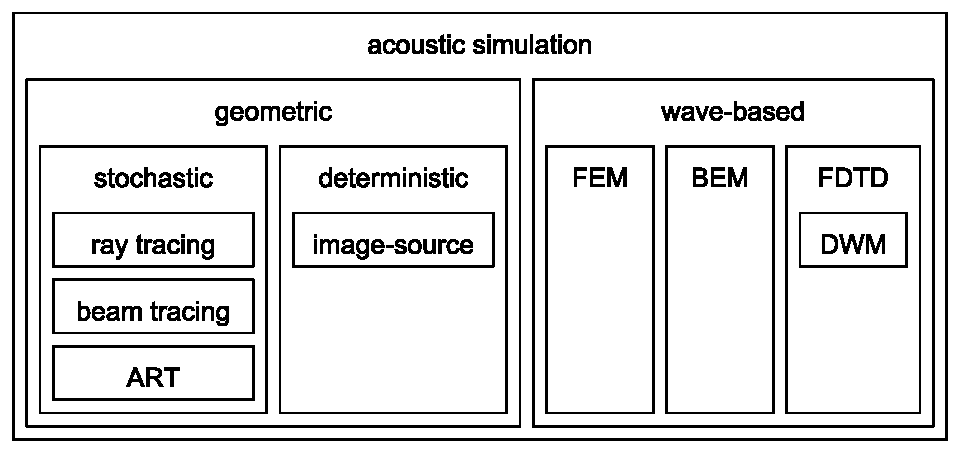
\includegraphics{images/simulation_techniques.pdf}
\caption{An overview of different acoustic simulation methods, grouped
by category.\label{fig:simulation_techniques}}
\end{figure}

\subsection{Geometric Methods}\label{geometric-methods}

Geometric methods can be grouped into two categories: \emph{stochastic}
and \emph{deterministic}.

Stochastic methods are generally based on statistical approximation via
some kind of Monte Carlo method. Such methods are approximate by nature.
They aim to randomly and repeatedly sample the problem space, recording
samples which fulfil some correctness criteria, and discarding the rest.
By combining the results from multiple samples, the probability of an
incorrect result is reduced, and the accuracy is increased. The balance
of quality and speed can be adjusted in a straightforward manner, simply
by adjusting the number of samples taken.

In room acoustics, stochastic algorithms may be based directly on
reflection paths, using \emph{ray tracing} or \emph{beam tracing}, in
which rays or beams are considered to transport acoustic energy around
the scene. Alternatively, they may use a surface-based technique, such
as \emph{acoustic radiance transfer} (ART), in which surfaces are used
as intermediate stores of acoustic energy.

Surface-based methods, especially, are suited to real-time simulations
(i.e.~interactive, where the listener position can change), as the
calculation occurs in several passes, only the last of which involves
the receiver object. This means that early passes can be computed and
cached, and only the final pass must be recomputed if the receiver
position changes.

The main deterministic method is the \emph{image source} method, which
is designed to calculate the exact reflection paths between a source and
a receiver. For shoebox-shaped rooms, and perfectly rigid surfaces, it
is able to produce an exact solution to the wave equation. However, by
its nature, it can only model specular (perfect) reflections, ignoring
diffuse and diffracted components. For this reason, it is inexact for
arbitrary enclosures, and unsuitable for calculating reverb tails, which
are predominantly diffuse. The technique also becomes prohibitively
expensive beyond low orders of reflection. The naive implementation
reflects the sound source against all surfaces in the scene, resulting
in a set of \emph{image sources}. Then, each of these image sources is
itself reflected against all surfaces. For high orders of reflection,
the required number of calculations quickly becomes impractical. For
these reasons, the image source method is only suitable for early
reflections, and is generally combined with a stochastic method to find
the late part of an impulse response.

For a detailed reference on geometric acoustic methods, see
{[}\protect\hyperlink{ref-saviojaux5foverviewux5f2015}{2}{]}.

\subsection{Wave-based Methods}\label{wave-based-methods}

The main advantage of wave-based methods is that they inherently account
for wave effects such as diffraction and interference
{[}\protect\hyperlink{ref-shelleyux5fdiffuseux5f2007}{5}{]}, while
geometric methods do not. This means that these wave-based methods are
capable of accurately simulating the low-frequency component of a room
impulse-response, where constructive and destructive wave interference
form \emph{room modes}. Room modes have the effect of amplifying and
attenuating specific frequencies in the room impulse response, and
produce much of the subjective sonic ``colour'' or ``character'' of a
room. Reproducing these room modes is therefore vital for evaluating the
acoustics of rooms such as concert halls and recording studios, or when
producing musically pleasing reverbs.

Wave-based methods may be derived from the \emph{Finite Element Method}
(FEM), \emph{Boundary Element Method} (BEM) or \emph{Finite-Difference
Time-Domain} (FDTD) method. The FEM and BEM are known together as
\emph{Element Methods}.

The FEM is an iterative numerical method for finding natural resonances
of a bounded enclosure. It models the air pressure inside the enclosure
using a grid of interconnected nodes, each of which represents a
mechanical system with a single degree of freedom. The
interconnectedness of the nodes leads to a set of simultaneous
equations, which can be solved for displacement at each node, and then
the solved equations can be used to calculate pressure values at certain
elements. The BEM is similar, but models nodes on the surface of the
enclosure, instead of within it. This in turn allows it to model
unbounded spaces, whereas the FEM is limited to bounded spaces
{[}\protect\hyperlink{ref-murphyux5fdigitalux5f2000}{6}, pp. 52--55{]}.

The FDTD method works by dividing the space to be modelled into a
regular grid, and computing changes in some quantity (such as pressure
or particle velocity) at each grid point over time. The formula used to
update each grid point, along with the topology of the grid, may be
varied depending on the accuracy, efficiency, and complexity required by
the application. FDTD methods are generally applied to problems in
electromagnetics, but a subclass of the FDTD method known as the
\emph{Digital Waveguide Mesh} (DWM) is often used for solving acoustics
problems.

The FDTD process shares some characteristics with the element methods.
They all become rapidly more computationally expensive as the maximum
output frequency increases
{[}\protect\hyperlink{ref-valimakiux5ffiftyux5f2012}{7}{]}. They also
share the problem of discretisation or quantisation, in which details of
the modelled room can only be resolved to the same accuracy as the
spatial sampling period. If a large inter-element spacing is used,
details of the room shape will be lost, whereas a small spacing will
greatly increase the computational load.

The major advantage of FDTD over element methods is that it is run
directly in the time domain, rather than producing frequency-domain
results, which in turn affords a much simpler implementation.

FDTD simulations can also be implemented with relative efficiency by
taking advantage of their ``embarrassingly parallel'' nature. Each
individual node in the simulation (of which there may be thousands or
millions) can be updated without synchronisation. As a result, the nodes
may be updated entirely in parallel, leading to massive reductions in
simulation time.

The main disadvantage of the FDTD method is that it is susceptible to
\emph{numerical dispersion}, in which wave components travel at
different speeds depending on their frequency and direction, especially
at high frequencies. Several techniques exist to reduce this error, such
as oversampling the mesh
{[}\protect\hyperlink{ref-camposux5fcomputationalux5f2005}{8}{]}, using
different mesh topologies
{[}\protect\hyperlink{ref-saviojaux5freductionux5f1999}{9}{]},
{[}\protect\hyperlink{ref-vanux5fduyneux5ftetrahedralux5f1995}{10}{]},
and post-processing the simulation output
{[}\protect\hyperlink{ref-saviojaux5finterpolatedux5f2001}{11}{]}.
Oversampling further increases the computational load of the simulation,
while using different topologies and post-processing both introduce
additional complexity.

Despite its drawbacks, the FDTD method is generally preferred for room
acoustics simulation
{[}\protect\hyperlink{ref-valimakiux5ffiftyux5f2012}{7}{]}, due to its
straightforward implementation, inherent parallelism, intuitive
behaviour, and its ability to directly produce time-domain impulse
responses.

\section{Existing Software}\label{existing-software}

A handful of programs exist for acoustic simulation. The following table
\text{(\ref{tab:software})} shows a selection which, whilst not
exhaustive, is representative.

\begin{table}[ht]
\centering

\caption{Some of the most prominent tools for acoustic
simulation.\label{tab:software}}

\begin{tabular}{@{}lll@{}}
\toprule

Name & Type & Availability \\\midrule

Odeon
{[}\protect\hyperlink{ref-ux5fodeonux5f2016}{12}{]} & Geometric & Commercial \\
CATT-Acoustic
{[}\protect\hyperlink{ref-ux5fcatt-acousticux5f2016}{13}{]} & Geometric & Commercial \\
Olive Tree Lab
{[}\protect\hyperlink{ref-ux5fotlux5f2016}{14}{]} & Geometric & Commercial \\
EASE
{[}\protect\hyperlink{ref-ux5feaseux5f2016}{15}{]} & Geometric & Commercial \\
Auratorium
{[}\protect\hyperlink{ref-ux5faudiobornux5f2016}{16}{]} & Geometric & Commercial \\
RAVEN
{[}\protect\hyperlink{ref-schroderux5fraven:ux5f2011}{17}{]} & Geometric & None \\
RoomWeaver
{[}\protect\hyperlink{ref-beesonux5froomweaver:ux5f2004}{18}{]} & Waveguide & None \\
EAR
{[}\protect\hyperlink{ref-ux5fearux5f2016}{19}{]} & Geometric & Free \\
PachydermAcoustic
{[}\protect\hyperlink{ref-ux5fpachydermux5f2016}{20}{]} & Geometric & Free \\
Parallel FDTD
{[}\protect\hyperlink{ref-ux5fparallelfdtdux5f2016}{21}{]} & Waveguide & Free \\
i-Simpa
{[}\protect\hyperlink{ref-ux5fi-simpaux5f2016}{22}{]} & Geometric,
extensible & Free \\

\bottomrule
\end{tabular}

\end{table}

All commercial acoustics programs found use geometric techniques,
probably because they are fast to run, and can often be implemented to
run interactively, in real-time. However, low-frequency performance is a
known issue with these programs. For example, the FAQ page for the Odeon
software {[}\protect\hyperlink{ref-ux5fodeonux5f2016-1}{23}{]} notes
that:

\begin{quote}
For Odeon simulations as with real measurements, the source and receiver
should be at least 1/4th wave length from the walls. But at the very
lowest resonance of the room the level can change a lot from position to
position without Odeon being able to predict it. For investigation of
low frequency behavior (resonances), indeed Odeon is not the tool.
\end{quote}

Clearly there is a need for wave-modelling acoustics software, which can
accurately predict low frequency behaviour. However, such software seems
to be somewhat rarer than geometric acoustics software. Of the two
wave-modelling programs listed, only one is generally available, which
must additionally be run from Python or Matlab scripts. This is a good
approach for research software, but would probably not be
straightforward for users with limited programming experience.

At time of writing (December 2016) it appears that no
generally-available (commercially or otherwise) piece of software has
taken the approach of combining wave-modelling and geometric methods,
although this technique is well-known in the literature
{[}\protect\hyperlink{ref-southernux5fspatialux5f2011}{1}{]},
{[}\protect\hyperlink{ref-aretzux5fcombinedux5f2009}{4}{]},
{[}\protect\hyperlink{ref-southernux5fhybridux5f2013}{24}{]}--{[}\protect\hyperlink{ref-vorlanderux5fsimulationux5f2009}{27}{]}.

\section{Project Aims}\label{project-aims}

The fundamental goals of the project are:

\begin{itemize}
\tightlist
\item
  \textbf{Accuracy}: Provide a way of generating accurate impulse
  responses of arbitrary enclosed spaces.
\item
  \textbf{Efficiency}: Ensure that the simulation is fast. Simulations
  times should be minutes, rather than hours or days.
\item
  \textbf{Accessibility}: It should be possible for someone with no
  programming experience to generate impulse responses. It should also
  be possible for other programmers to extend and modify the project's
  code.
\end{itemize}

The project is primarily designed to help musicians and sound designers,
who require high-quality reverberation effects. These users also need
fast iteration times between making parameter adjustments and hearing
the results, so that the ``right'' sound can be created quickly. The
solution must run on commodity hardware, as musicians are not expected
to have access to dedicated compute clusters or server farms.

Accuracy and efficiency are competing goals, which must be balanced.
Extreme performance, allowing real-time usage, has already been
implemented in several of the commercial programs listed above, and
generally relies on simplified acoustic models, which in turn reduce
accuracy. This runs counter to the aims of the project. Similarly,
extreme accuracy generally requires long compute times and specialised
hardware, both of which are inaccessible to the target user. Therefore,
the focus of the project cannot be solely on accuracy. Software which
balances these two aims does not exist, at time of writing, and there is
a clear need for a solution which is both reasonably fast and accurate.

Accessibility is extremely important, and the final product must be
accessible to two main groups. Firstly, it must be useful to the target
users. It must be simple to install and run, and should not require
specialist training in acoustics or programming. Secondly, the code and
supporting materials must be made free to researchers, to encourage
further research and modification.

\subsection{Proposed Solution}\label{proposed-solution}

It appears that an approach combining geometric and wave-based methods
will be most flexible in achieving both accuracy and efficiency:
wave-based methods are accurate but slow; and geometric methods are
faster but less accurate. Accuracy and efficiency can be balanced by
adjusting the proportion of the output generated with each method. The
Wayverb project puts forward an acoustic simulator based on this hybrid
method.

To achieve the goal of accessibility, the Wayverb program runs on
consumer hardware, and is accessed through a graphical interface which
allows simulations to be configured, stored, and run. Code for the
project is public and permissively licensed.

\section{Original Contributions}\label{original-contributions}

Most importantly, at time of writing, Wayverb is the only public
graphical acoustics tool incorporating geometric and wave-based methods.
Although hybrid acoustics methods are well documented
{[}\protect\hyperlink{ref-aretzux5fcombinedux5f2009}{4}{]},
{[}\protect\hyperlink{ref-southernux5fhybridux5f2013}{24}{]},
{[}\protect\hyperlink{ref-murphyux5fhybridux5f2008}{25}{]}, they have
only been used in specific research settings, for producing experimental
results. It may be assumed that these tools have been built to model
specific test-cases, rather than general simulation tasks, but this is
uncertain as no tools incorporating these techniques have been made
public. However, Wayverb is able to model arbitrary enclosures.

The project acts as a survey of room acoustics techniques, and related
issues regarding practical implementation. Rather than designing
completely new simulation methods, existing techniques were
investigated, compared, and evaluated in terms of their accuracy and
performance. Then, optimum techniques were chosen and further developed
for use in the final program. An especially important consideration is
the matching of parameters between models. For example, all models
should produce the same sound energy at a given distance, and should
exhibit the same reverb time for a given scene. Therefore, the acoustics
techniques were chosen so that they produce consistent results.

Sometimes the models required development beyond the methods presented
in the literature in order to become useful. An example of this is the
waveguide set-up process. Most experimental set-ups in the literature
only model cuboid-shaped enclosures, and no guidance is given for
setting up simulations in arbitrarily-shaped enclosures. Of course, it
must be possible to model real, complex room shapes, and so an original
set-up procedure had to be developed. The same goes for memory layout
and implementation details: in the literature, techniques for efficient
implementation are rarely discussed. As a result, new techniques had to
be invented, rather than reimplementing known methods. Where extensions
to existing techniques have been developed for use in Wayverb, this is
mentioned in the text.

Much of the literature on acoustic simulation focuses predominantly on
accuracy. Performance appraisals are rarely given, presumably because
they are somewhat subjective, and ``reasonable'' efficiency will vary
between applications. Ideally, the simulation methods in Wayverb should
be selected and implemented to allow tunable performance, so that
results with acceptable accuracy can be generated within a few minutes,
but it is possible to run longer simulations if higher-accuracy results
are needed. This is similar to approaches taken in computer graphics,
where ``overview'' renders may take seconds to generate, but
physically-modelled simulations for film often take hours to render,
even on purpose-built compute clusters.

The notable components of the Wayverb project are as follows, each of
which has a dedicated chapter with detailed explanation:

\begin{itemize}
\tightlist
\item
  Image-source model, accelerated with parallel ray-casting, for early
  reflections. Uses a novel method for speeding up audibility tests by
  re-using reflection paths from the ray tracer.
\item
  Parallel stochastic ray-tracer, for late reflections.
\item
  Parallel digital waveguide mesh, for low frequency modelling. Uses a
  novel set-up procedure to create meshes with correctly-placed boundary
  nodes in arbitrary scenes.
\item
  Calibration, automatically matching the output levels of the different
  models.
\item
  A microphone model, capable of simulating capsules with
  direction-dependent frequency responses, within all three
  simulation-types.
\item
  A boundary model with matched performance in all three
  simulation-types.
\end{itemize}

\subsection{Chosen Simulation
Techniques}\label{chosen-simulation-techniques}

The image-source and stochastic ray-tracing methods were chosen for
modelling high-frequency content. These models are complementary: the
image model can find early reflections with great accuracy but is slow
at finding later reflections; while the ray-tracer is much faster but
more approximate, making it better suited to finding naturally-diffuse
late reflections. Specifically, a simple ray tracing method was chosen
over a phonon- or surface-based method for the late-reflection
simulation, for several reasons. Firstly, ray tracing is broadly
discussed in the literature
{[}\protect\hyperlink{ref-krokstadux5fcalculatingux5f1968}{28}{]}--{[}\protect\hyperlink{ref-alpkocakux5fcomputingux5f2010}{32}{]},
so would not require a great deal of experimentation to implement.
Secondly, ray tracing has the property of being an \emph{embarrassingly
parallel} algorithm, because each individual ray can be simulated
entirely independently, without requiring communication or
synchronisation. By running the algorithm on graphics hardware, which is
designed to run great numbers of calculations in parallel, all rays
could be simulated in one go, yielding much greater performance than
processing each ray sequentially. Finally, though surface-based methods
are capable of real-time operation, they do not pose any performance
benefit for non-real-time or ``one-off'' simulations. Their performance
comes from re-using pre-computed information when the receiver position
changes, but in a one-off simulation the receiver position is fixed. Ray
tracing is also less complex and better documented than surface-based
methods, making it the superior choice for this application. A
logistical reason for choosing the image-source and ray tracing solution
for high-frequency modelling was that the author had previously
implemented such a system for an undergraduate project. It was hoped
that much of the code from that project could be re-used, but it
transpired that the project suffered from accuracy and implementation
issues, making it unsuitable for direct integration within Wayverb.
Therefore, the majority of this code was completely re-written. The
author was, however, able to re-use much of the knowledge and experience
gained from the previous project, which would not have been possible if
a completely new stochastic method had been introduced.

For low-frequency simulation, a FDTD-based DWM model was chosen. There
is a great deal of writing on this method
{[}\protect\hyperlink{ref-murphyux5fdigitalux5f2000}{6}{]},
{[}\protect\hyperlink{ref-camposux5fcomputationalux5f2005}{8}{]},
{[}\protect\hyperlink{ref-vanux5fduyneux5f3dux5f1996}{33}{]}--{[}\protect\hyperlink{ref-kowalczykux5froomux5f2011}{35}{]},
it is relatively simple to implement, and shares with ray tracing the
characteristic of being embarrassingly parallel. As wave-modelling is
especially costly, a parallel implementation is necessary in order to
achieve simulation times in the order of minutes rather than hours or
days.

An in-depth description of the algorithms implemented is given in the
\href{\%7B\%7B\%20site.baseurl\%20\%7D\%7D\%7B\%\%20link\%20image_source.md\%20\%\%7D}{Image-Source},
\href{\%7B\%7B\%20site.baseurl\%20\%7D\%7D\%7B\%\%20link\%20ray_tracer.md\%20\%\%7D}{Ray
Tracer}, and
\href{\%7B\%7B\%20site.baseurl\%20\%7D\%7D\%7B\%\%20link\%20waveguide.md\%20\%\%7D}{Waveguide}
sections. The following figure \text{(\ref{fig:regions})} shows how the
outputs from the different methods work together to produce a broadband
impulse response. It shows that the lower portion of the spectrum is
generated entirely with the waveguide, while the upper portion is
simulated using the image-source method for early reflections, and the
ray tracing method for the reverb tail.

\begin{figure}[htbp]
\centering
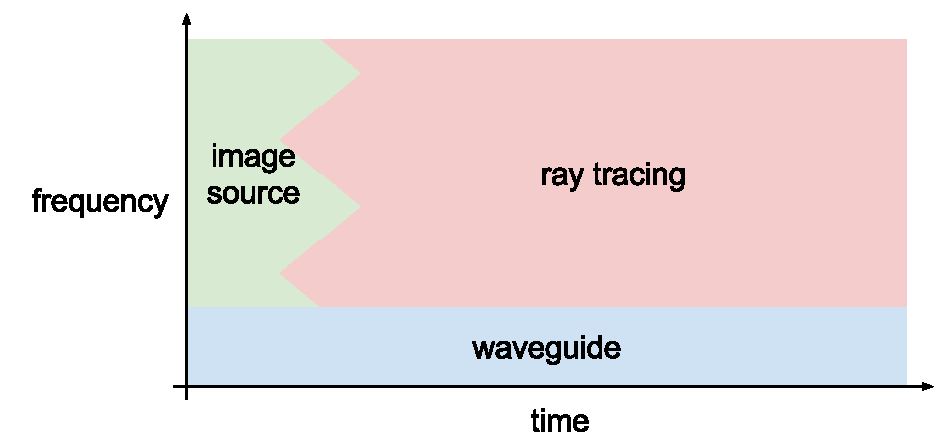
\includegraphics{images/regions.pdf}
\caption{The structure of a simulated impulse
response.\label{fig:regions}}
\end{figure}

Deciding on the simulation techniques led to three questions:

\begin{itemize}
\tightlist
\item
  To produce a final output, the three simulations must be automatically
  mixed in some way. How can this be done?
\item
  Binaural simulation requires some method for direction- and
  frequency-dependent attenuation at the receiver. How can receivers
  with polar patterns other than omnidirectional be modelled
  consistently in all three simulation methods?
\item
  The reverb time and character depends heavily on the nature of the
  reflective surfaces in the scene. How can frequency-dependent
  reflective boundaries be modelled consistently in all methods?
\end{itemize}

These questions will be discussed in the
\href{\%7B\%7B\%20site.baseurl\%20\%7D\%7D\%7B\%\%20link\%20hybrid.md\%20\%\%7D}{Hybrid},
\href{\%7B\%7B\%20site.baseurl\%20\%7D\%7D\%7B\%\%20link\%20microphone.md\%20\%\%7D}{Microphone
Modelling}, and
\href{\%7B\%7B\%20site.baseurl\%20\%7D\%7D\%7B\%\%20link\%20boundary.md\%20\%\%7D}{Boundary
Modelling} sections respectively.

\subsection{Chosen Technology}\label{chosen-technology}

The programming language chosen was C++. For acceptable performance in
numerical computing, a low-level language is required, and for rapid
prototyping, high-level abstractions are necessary. C++ delivers on both
of these requirements, for the most part, although its fundamentally
unsafe memory model does introduce a class of bugs which do not really
exist in languages with garbage collection, borrow checking, or some
other safety mechanism.

OpenCL was chosen for implementing the most parallel parts of the
simulation. The OpenCL framework allows a single source file to be
written, in a C-like language, which can target either standard
\emph{central processing units} (CPUs), or highly parallel
\emph{graphics processing units} (GPUs). The main alternative to OpenCL
is CUDA, which additionally can compile C++ code, but which can only
target Nvidia hardware. OpenCL was chosen as it would allow the final
program to be run on a wider variety of systems, with fewer limitations
on their graphics hardware.

The only deployment target was Mac OS. This was mainly to ease
development, as maintaining software across multiple platforms is often
time-consuming. Mac OS also tends to have support for newer C++ language
features than Windows, which allows code to be more concise, flexible,
and performant.\footnote{Visual Studio 2015 for Windows still does not
  support all of the C++11 language features
  {[}\protect\hyperlink{ref-ux5fvisualux5f2016}{36}{]}, while the Clang
  compiler used by Mac OS has supported newer C++14 features since
  version 3.4 {[}\protect\hyperlink{ref-ux5fclangux5f2016}{37}{]},
  released in May 2014
  {[}\protect\hyperlink{ref-ux5fdownloadux5f2016}{38}{]}.} Targeting a
single platform avoids the need to use only the lowest common
denominator of language features. As far as possible, the languages and
libraries have been selected to be portable if the decision to support
other platforms is made in the future.

The following additional libraries were used to speed development. They
are all open-source and freely available.

\begin{description}
\tightlist
\item[GLM]
Provides vector and matrix primitives and operations, primarily designed
for use in 3D graphics software, but useful for any program that will
deal with 3D space.
\item[Assimp]
Used for loading and saving 3D model files in a wide array of formats,
with a consistent interface for querying loaded files.
\item[FFTW3]
Provides Fast Fourier Transform routines. Used mainly for filtering and
convolution.
\item[Libsndfile]
Used for loading and saving audio files, specifically for saving
simulation results.
\item[Libsamplerate]
Provides high-quality sample-rate-conversion routines. Waveguide
simulations are often run at a relatively low sample-rate, which must
then be adjusted.
\item[Gtest]
A unit-testing framework, used to validate small individual parts of the
program, and ensure that changes to one module do not cause breakage
elsewhere.
\item[Cereal]
Serializes data to and from files. Used for saving program configuration
options.
\item[ITPP]
A scientific computing library. Used for its implementation of the
Yule-Walker method for estimating filter coefficients for a given
magnitude response.
\item[JUCE]
Provides a framework for building graphical applications in C++. Used
for the final application.
\end{description}

The project uses CMake to configure its build, and to automatically
download project dependencies. Python and Octave were used for running
and automating tests and generating graphs.

This documentation is written in Markdown, and compiled to html and to
pdf using Pandoc. The project website is generated with Jekyll.

\chapter{Image-source Model}\label{image-source-model}

\section{Background}\label{background}

\hypertarget{basic-method}{\subsection{Basic
Method}\label{basic-method}}

The image-source method aims to find the purely specular reflection
paths between a source and a receiver. This process is simplified by
assuming that sound propagates only along straight lines or rays. Sound
energy travels at a fixed speed, corresponding to the speed of sound,
along these rays. The energy in each ray decreases with \(1/r^2\), where
\(r\) is the total distance that the ray has travelled
{[}\protect\hyperlink{ref-vorlanderux5fauralization:ux5f2007}{30}, p.
58{]}.

Rays are perfectly reflected at boundaries. When a ray is reflected, it
spawns a secondary source ``behind'' the boundary surface. This source
is located on a line perpendicular to the wall, at the same distance
from it as the original source, as if the original source has been
``mirrored'' in the surface. This new ``image'' source now represents a
perfect reflection path, in that the distance along the straight line
between the receiver and the image source has the same length as the
path from the \emph{real} source to the receiver, reflected in the
boundary. If the source is reflected in a single boundary, this
represents a first-order reflection. A ray which is reflected from
several boundaries is represented by a ``higher-order'' image-source,
which has been mirrored in each of those boundaries in turn
{[}\protect\hyperlink{ref-kuttruffux5froomux5f2009}{29}, p. 104{]}.

\begin{figure}[htbp]
\centering
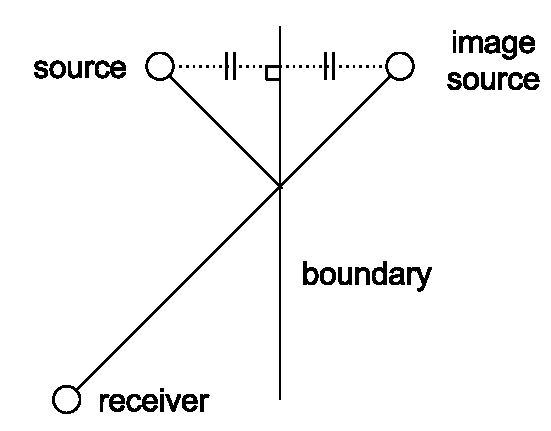
\includegraphics{images/image_source_construction.pdf}
\caption{Image sources are found by reflecting the source position in a
boundary.\label{fig:image_source_construction}}
\end{figure}

All sources, original and image, emit the same impulsive source signal
at the same time. The total impulse response (i.e.~sound pressure
against time) is found by summing the signals from each source, delayed
and attenuated appropriately depending on the distance between that
source and the receiver, which is equivalent to the length of the
specular reflection path. The frequency response of the signal from each
image source will additionally be modified depending on the
characteristics of each boundary in which that source was reflected.

In the real world, not all energy is perfectly reflected at a boundary.
Some energy will be randomly diffused in non-specular directions. The
image-source model is not capable of modelling this phenomenon, though
this is not particularly problematic. Consider that, once scattered,
sound energy cannot become un-scattered. The conversion from incoming
energy to scattered energy is unidirectional, so repeated reflections
cause the ratio of scattered to specular energy to increase
monotonically. Kuttruff shows that, though the earliest reflections may
be largely specular, after a few reflections the large majority of sound
energy becomes diffuse
{[}\protect\hyperlink{ref-kuttruffux5froomux5f2009}{29}, p. 126{]}. This
suggests that the image model should be used only for very early
reflections, where most energy is not scattered, and a secondary model
used to compute late, diffuse reflections. In Wayverb, the image model
is used for early reflections, and stochastic ray-tracing is used for
the diffuse tail. The combination of the two models is described in the
\href{\%7B\%7B\%20site.baseurl\%20\%7D\%7D\%7B\%\%20link\%20hybrid.md\%20\%\%7D}{Hybrid
Model} section.

\subsection{Audibility Checking}\label{audibility-checking}

The position of an image source is found by reflecting it in one or more
surfaces. Next, it must be checked to ensure it represents a valid
specular path to the receiver. This is known as an \emph{audibility
test} {[}\protect\hyperlink{ref-vorlanderux5fauralization:ux5f2007}{30},
p. 202{]}.

Consider first a source \(S\), a receiver \(R\), and a single wall
\(A\). The source is reflected in \(A\), creating an image-source
\(S_A\). A line is constructed from \(R\) to \(S_A\). If this line
intersects \(A\), then \(S_A\) represents a valid image source.
Otherwise, there is no possible specular reflection involving \(S\),
\(R\) and \(A\).

Now consider two walls, \(A\) and \(B\). The image source \(S_{AB}\) has
been reflected in \(A\) then \(B\). For the image-source to be valid:

\begin{itemize}
\tightlist
\item
  \(R \rightarrow S_{AB}\) must intersect \(B\) at some point
  \(B_\text{intersection}\),
\item
  \(B_\text{intersection} \rightarrow S_A\) must intersect \(A\) at
  \(A_\text{intersection}\), \emph{and}
\item
  \(A_\text{intersection} \rightarrow S\) must not intersect with any
  scene geometry.
\end{itemize}

The validation of a third-order image-source will require three
intersection checks, a fourth-order image will require four checks, and
so on. This method of tracing backwards from the receiver to each of the
image sources is known as \emph{backtracking}.

\begin{figure}[htbp]
\centering
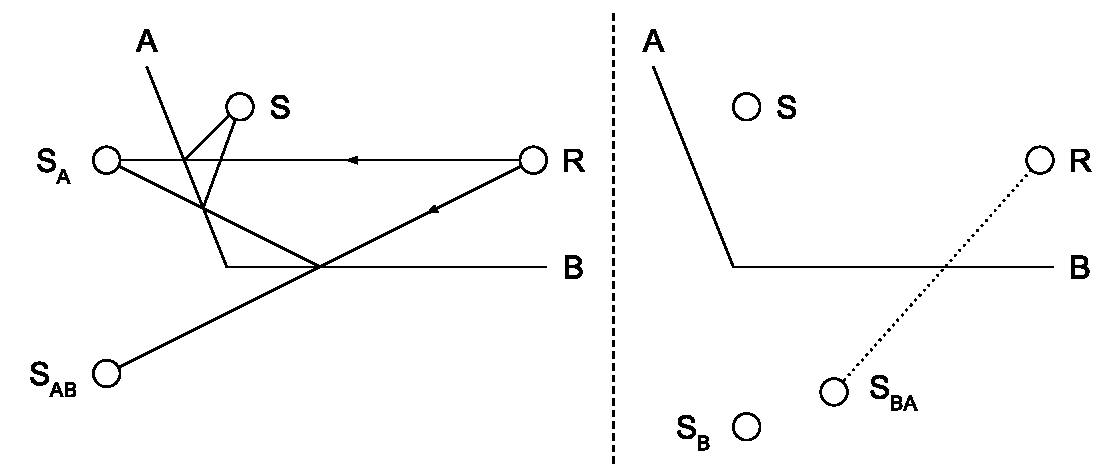
\includegraphics{images/backtracking.pdf}
\caption{\textbf{Left:} The paths \(S \rightarrow A \rightarrow R\) and
\(S \rightarrow A \rightarrow B \rightarrow R\) are both valid.
\textbf{Right:} \(S \rightarrow B \rightarrow A \rightarrow R\) is an
invalid path because \(R \rightarrow S_{BA}\) does not intersect
\(A\).\label{fig:backtracking}}
\end{figure}

\subsection{Accelerating the
Algorithm}\label{accelerating-the-algorithm}

The naive method to find all the image sources for a scene is very
expensive: Consider that to find a single first-order image source, the
original source must be mirrored in a surface, and then an intersection
test must be conducted between that surface and the
image-source-to-receiver ray. To find all first-order image sources,
this process must be carried out for all surfaces in the scene. To find
all second-order image sources, each of those first-order images must be
tested against every surface. This continues for higher-order images, so
that the number of checks for image sources of a given order is equal to
the number of surfaces raised to the power of that order. The
relationship between the image-source order and the computation time is
therefore exponential, with average-case complexity of \(O(N^o)\) where
\(N\) denotes the number of boundaries, and \(o\) is the image-source
order. As a result, it is impossible to validate all possible
image-source positions within a reasonable time.

The majority of higher-order image sources found with the naive
algorithm will be invalid. That is, they will fail the audibility test.
For example, for tenth-order image-sources in a shoebox-shaped room,
there are around 1.46e7 different image sources, only 1560 of which are
valid {[}\protect\hyperlink{ref-kuttruffux5froomux5f2009}{29}, p.
323{]}. If the invalid image-sources can be discarded early, without
requiring individual checking, then the amount of computation can be
greatly reduced to a viable level. As explained above, image sources
above order four or five are rarely required, but even these can be very
time-consuming to find with the naive method. Optimisations are,
therefore, a necessity for all but the simplest simulations.

To accelerate the image-source process,
{[}\protect\hyperlink{ref-vorlanderux5fauralization:ux5f2007}{30}{]}
suggests tracing a large number of rays in random directions from the
source, and logging the unique paths of rays which eventually intersect
with the receiver. The complexity of ray tracing grows linearly rather
than exponentially with reflection depth, meaning it can find deeper
reflections with far fewer operations than the image-source method. Each
unique path found in this way is used to generate an image source
sequence, which is then checked as normal. This technique has the
advantage that the majority of surface sequences are \emph{not} checked,
so the image-source process is fast. However, if the preliminary
ray-tracer is not run with enough rays, it is likely to miss some valid
paths, especially in complex scenes. Additionally, if the receiver
volume is too great, then some invalid paths may still be detected.

The technique used by Wayverb is similar to that presented in
{[}\protect\hyperlink{ref-vorlanderux5fauralization:ux5f2007}{30}{]},
but makes a small change to the acceleration process. Note that this
does not affect the physical interpretation of the image-source model.
It simply changes the way in which ray paths are initially selected for
further audibility checking.

A large number of random rays are traced, as before, but at each
reflection point, the receiver is checked to see whether it is visible.
If it is, then the surface sequence is checked for a valid image-source.
This adds constant work per-reflection to the ray-tracing process, which
is insignificant in terms of overall time-complexity. This technique has
two main advantages. Firstly, more paths are checked, so it is more
likely to find all the valid image-sources. Instead of just checking ray
paths which intersect the receiver, this method checks all paths which
are \emph{capable} of intersecting the receiver. Secondly, initial ray
paths don't have to be specular, so techniques like \emph{vector-based
scattering} can be used. The disadvantage is that a greater number of
validity checks are required, though this number is still many times
smaller than would be required by a naive implementation.

\section{Implementation}\label{implementation}

Here the concrete implementation of the image-source method is
presented, as it is used in Wayverb. The following figure
\text{(\ref{fig:image_source_process})} gives an overview of the entire
process.

\begin{figure}[htbp]
\centering
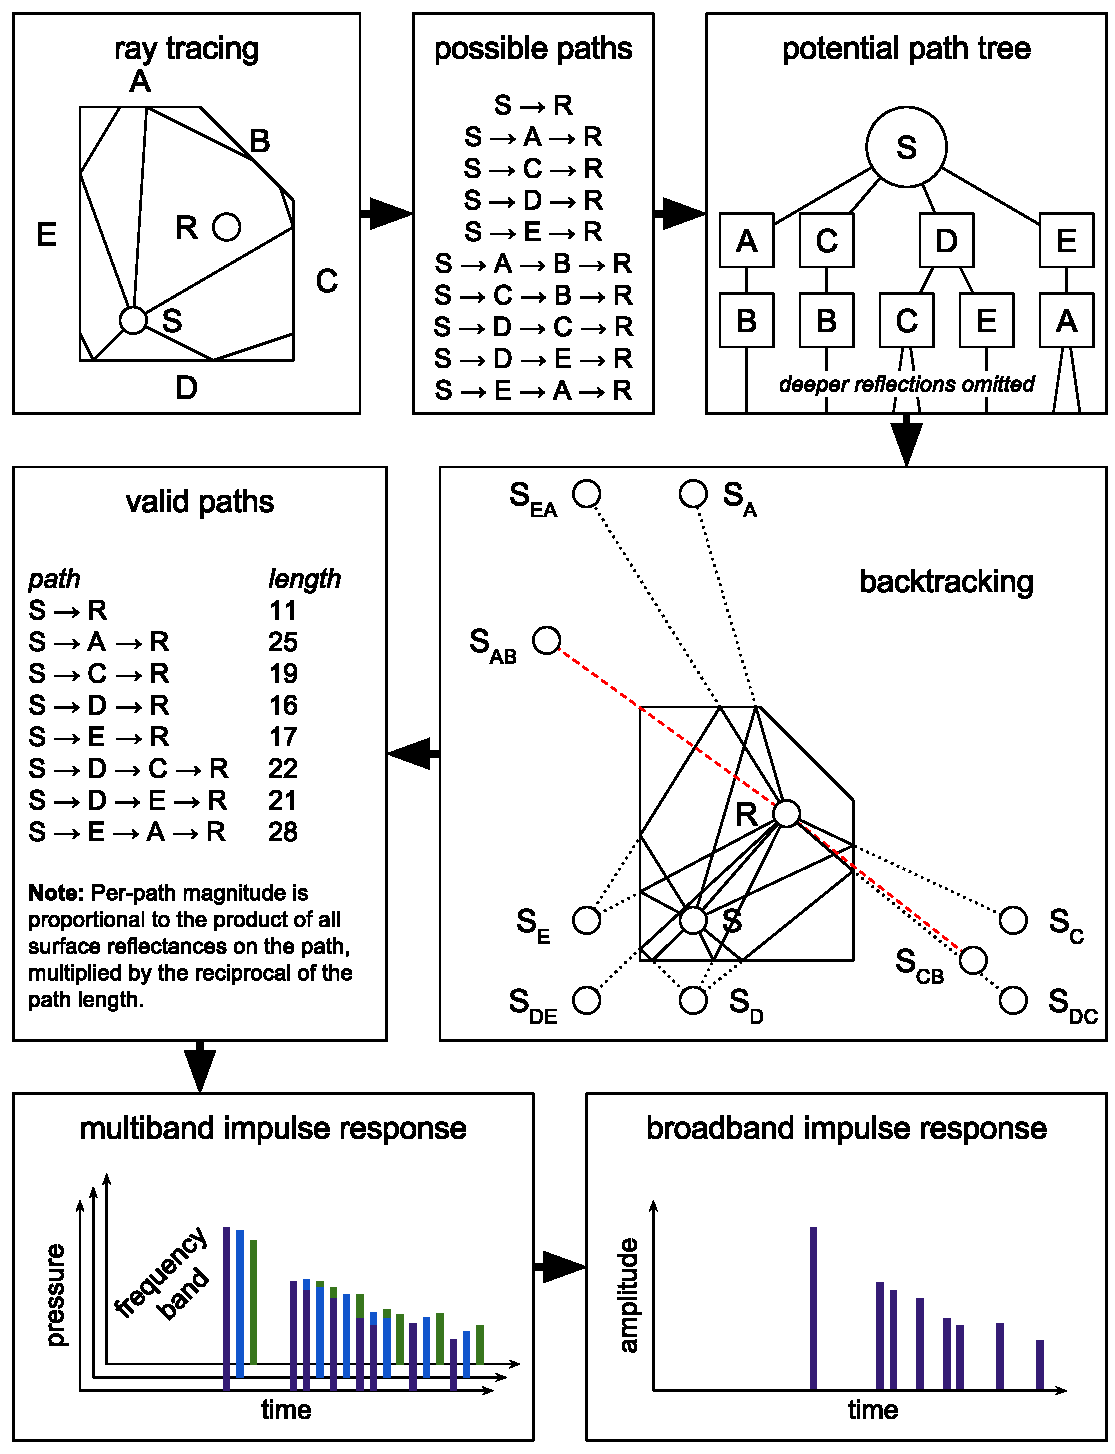
\includegraphics{images/image_source_process.pdf}
\caption{Creation of an impulse response using image
sources.\label{fig:image_source_process}}
\end{figure}

The main prerequisite for the simulation is a scene, made up of
triangles, where each triangle has an associated material comprised of
multi-band absorption coefficients. First, an axis-aligned bounding box
is computed for this scene, and split into uniformly sized cuboid
\emph{voxels}. Each voxel holds a reference to any triangles in the
scene which happen to intersect with that voxel. The voxel mesh acts as
an ``acceleration structure'', speeding up intersection tests between
rays and triangles. To check for an intersection between a ray and a
number of triangles, the simplest method is to check the ray against
each triangle individually, which is very time consuming. The voxel mesh
allows the number to checks to be greatly reduced, by checking only
triangles that are within voxels that the ray intersects. These voxels
can be found very quickly, by ``walking'' the voxels along the ray,
using an algorithm presented by Amanatides, Woo et al.
{[}\protect\hyperlink{ref-amanatidesux5ffastux5f1987}{39}{]}. For large
scenes with many triangles, this method can lead to speed-ups of an
order of magnitude or more. All ray-intersection tests mentioned
throughout this thesis use the voxel-acceleration method, unless
explicitly noted. In particular, both the initial ray-casting \emph{and}
the image-source audibility-checking are accelerated using the voxel
method.

Rays are fired in uniform random directions from the source (item 1 in
the figure). Each ray is checked for an intersection with the scene, and
if an intersection is found, some data about the intersection is
recorded. Specifically, the record includes the triangle which was
intersected, and whether or not the receiver is visible from the
intersection point. Then, the vector-based scattering method
{[}\protect\hyperlink{ref-christensenux5fnewux5f2005}{40}{]} (see the
\href{\%7B\%7B\%20site.baseurl\%20\%7D\%7D\%7B\%\%20link\%20ray_tracer.md\%20\%\%7D}{Ray
Tracing} section for details on this) is used to find the directions of
new rays, which are fired from the intersection points. The ray-tracing
process continues up to a certain depth, which is artificially limited
to ten reflections in Wayverb. For most simulations, three or four
reflections should be adequate, though this depends somewhat on the
scattering coefficients of the surfaces. After a few reflections, most
sound energy is diffuse rather than specular, and other methods are
better suited to modelling this scattering, as explained in the
\protect\hyperlink{basic-method}{Basic Method} subsection above.

The ray tracer produces a list of reflection paths for each ray, where a
single reflection path is defined by a sequence of visited surfaces
(item 2 in the figure). Some rays may follow the same paths (reflect
from the same surfaces), and so duplicate paths must be removed. This is
achieved by condensing per-ray information into a tree of valid paths
(item 3). Each node in the tree stores a reference to a triangle in the
scene, and whether or not the receiver is visible from this triangle.
Each unique path starting from a root node in the tree represents a
possible image source contribution, which must be checked. This checking
is carried out using the backtracking method explained above (item 4).
The tree structure can be traversed using depth-first recursion,
allowing the results of some intermediate calculations to be cached
between ray paths, speeding up the calculation with only minimal memory
overhead. This is similar to the approach mentioned in
{[}\protect\hyperlink{ref-saviojaux5foverviewux5f2015}{2}{]}. Also,
because the tree is immutable, it can be shared between multiple worker
threads, which independently check each branch for valid image sources.
The nature of the recursive algorithm makes it a poor fit for an OpenCL
implementation, so native (CPU) threads are used instead.

Some paths in the tree may not actually produce valid image sources, and
these paths are discarded (item 5). For paths which \emph{do} contribute
valid image sources, the propagation delay and frequency-dependent
pressure of the image source signal must be found. As described by
Kuttruff, the propagation delay is equal to the distance from the
receiver to the image source, divided by the speed of sound,
{[}\protect\hyperlink{ref-kuttruffux5froomux5f2009}{29}, p. 325{]}. The
pressure content is found by convolving together the reflectances of all
intermediate surfaces. This is equivalent to a single multiplication per
frequency band, as long as the reflectance value for each band per
surface can be represented by a single real value.

The surface reflectances are found by converting per-band absorptions
into per-band normal-incidence reflectance magnitudes using

\begin{enumerate}
\def\labelenumi{(\arabic{enumi})}
\tightlist
\item
  \[|R|=\sqrt{1-\alpha}\]
\end{enumerate}

where \(R\) is the surface reflectance, and \(\alpha\) is the absorption
coefficient of that frequency band. These are converted to per-band
impedances \(\xi\) by

\begin{enumerate}
\def\labelenumi{(\arabic{enumi})}
\setcounter{enumi}{1}
\tightlist
\item
  \[\xi=\frac{1+|R|}{1-|R|}\]
\end{enumerate}

Finally, the impedances are converted back to \emph{angle-dependent}
reflectances by

\begin{enumerate}
\def\labelenumi{(\arabic{enumi})}
\setcounter{enumi}{2}
\tightlist
\item
  \[R(\theta)=\frac{\xi\cos\theta-1}{\xi\cos\theta+1}\]
\end{enumerate}

where \(\theta\) is the angle of incidence at the surface. This is the
same approach taken in
{[}\protect\hyperlink{ref-southernux5froomux5f2013}{26}{]}. \(\theta\)
must be found for each individual reflection, by taking the inverse
cosine of the dot product between the incident ray direction and the
surface normal, when both are unit vectors.

The contribution \(g\) of a single image source with intermediate
surfaces \(m_1 m_2 \dots m_n\) is given by

\begin{enumerate}
\def\labelenumi{(\arabic{enumi})}
\setcounter{enumi}{3}
\tightlist
\item
  \[g_{m_1 m_2 \dots m_n} = \frac{\sqrt{Z_0/4\pi}}{d_{m_1 m_2 \dots m_n}}
  \cdot R_{m_1} \ast R_{m_2} \ast \dots \ast R_{m_n} \ast \delta(\frac{d_{m_1 m_2
  \dots m_n}}{c})\]
\end{enumerate}

where \(Z_0\) is the acoustic impedance of air, \(c\) is the speed of
sound, \(d_{m_1 m_2 \dots m_n}\) is the distance from the receiver to
the image source, and \(R_{m_i}\) is the reflectance of surface \(i\).
This assumes that the original source emits a pressure impulse
\(\delta\) at the starting-time of the simulation. The contributions of
all image sources must be summed together to find the final impulse
response.

To create a digital audio file representing an impulse response, the
output must be discretised at some sampling frequency \(f_s\). The
individual image source contributions must be added, at positions
corresponding to their propagation delays, into an output buffer at that
sampling frequency. The ideal buffer position for a given contribution
is equal to \(\tau f_s\) where \(\tau\) is the propagation delay of that
contribution, equal to the total ray distance divided by the speed of
sound. However, this value is unlikely to be an integer, and so may not
coincide with a sample index. The simplest solution would be to round to
the closest integer, and use this as the sample index. However, for
applications such as multi-microphone simulation which are sensitive to
arrival time, this can lead to phase errors. A better solution is
suggested by Fu and Li
{[}\protect\hyperlink{ref-fuux5fgpu-basedux5f2016}{41}{]}: The
contribution can be positioned with sub-sample accuracy, by replacing
the impulsive \(\delta\) signal with the impulse-response of an ideal
low-pass filter, with cut-off equal to the output Nyquist frequency.
Such an impulse response is infinitely long, but tends to zero quickly,
so a Hann window can be applied to limit its length. This form of the
impulse is as follows:

\begin{enumerate}
\def\labelenumi{(\arabic{enumi})}
\setcounter{enumi}{4}
\tightlist
\item
  \[
  \delta_{\text{LPF}}(n - \epsilon)=
  \begin{cases}
  \frac{1}{2}(1+\cos\frac{2\pi (n - \epsilon)}{N_w})\text{sinc}(n - \epsilon), & - \frac{N_w}{2} < n < \frac{N_w}{2} \\
  0, & \text{otherwise}
  \end{cases} 
  \]
\end{enumerate}

where \(n\) is an index in the output buffer, \(\epsilon\) is the centre
of the impulse in samples (\(\epsilon=\tau f_s\)), and \(N_w\) is the
width of the window in samples.

Each image-source contribution has per-band pressure values. Rather than
summing all contributions directly to the output buffer, several buffers
are created, one per frequency band. The contributions for each band are
summed into each buffer individually (item 6 in the figure). The final
output of the simulation is created by band-passing and then mixing down
the buffers (item 7). A single method for multi-band filtering is used
throughout Wayverb, and more details are given in the
\href{\%7B\%7B\%20site.baseurl\%20\%7D\%7D\%7B\%\%20link\%20ray_tracer.md\%20\%\%7D}{Ray
Tracer} section.

\chapter{Ray Tracer}\label{ray-tracer}

\section{Background}\label{background-1}

Similarly to the image-source method, ray tracing assumes that sound
energy travels around a scene in ``rays''. The rays start at the sound
source, and are all emitted in uniformly random directions at the same
time, travelling at the speed of sound. When a ray hits a boundary, it
loses some of its energy, depending on the properties of the boundary's
material. Then, the ray is reflected. When it intersects the receiver,
the energy and time-delay of the ray is recorded. In these ways, the
models are similar. However, there are some important differences
between the two methods, explained below.

\subsection{Stochastic Simulation}\label{stochastic-simulation}

Image sources are deterministic, while ray tracing is stochastic. The
image-source method finds exact specular reflections, which are fixed
for given source, receiver, and boundary positions. Ray tracing is less
accurate, aiming to compute a result which is correct, within a certain
probability. A large number of rays are fired into the scene in random
directions, and traced until they have undergone a certain number of
reflections. Some of these rays may intersect with the receiver volume
(see below), but some may not. Only rays that \emph{do} intersect the
receiver contribute to the final output. The proportion of rays which
intersect the receiver, and therefore the measured energy at the
receiver, can be found with greater accuracy simply by increasing the
number of rays fired.

\subsection{Receiver Volume}\label{receiver-volume}

The random nature of ray tracing requires that the receiver must have a
finite volume. The likelihood of any given random ray intersecting with
a single point with no volume tends to zero (there is an infinite number
of possible ray directions, only one of which passes through the point).
If the probability of a ray-receiver intersection is to be non-zero, the
receiver must have some volume. This is different to the image-source
method, which traces reflections backwards from the receiver, allowing
it to be represented as a point.

\subsection{Energy and Distance}\label{energy-and-distance}

In ray tracing, each ray represents a finite portion of the initial
source energy. The reduction of energy over a given distance is
accounted for by the spreading-out of the rays. This can be illustrated
very simply: Imagine a sphere placed very close to a point. Assuming
rays are fired with a uniform random distribution from that point, a
certain proportion of those rays will intersect with the sphere. If the
sphere is moved further away, a smaller proportion of rays will hit it
(see the following figure \text{(\ref{fig:receiver_proximity})}).

\begin{figure}[htbp]
\centering
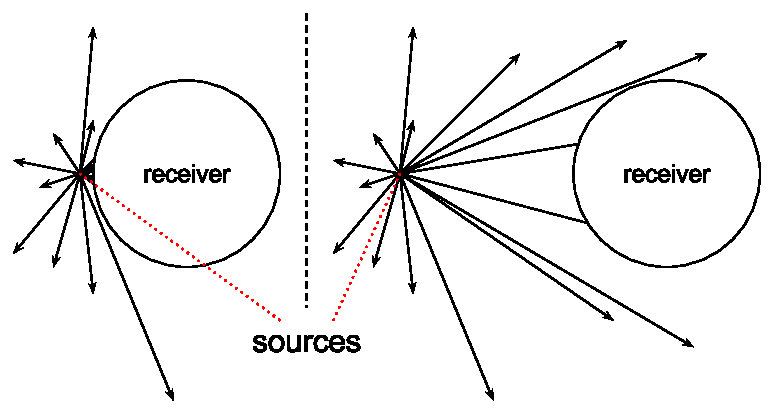
\includegraphics{images/receiver_proximity.pdf}
\caption{The proportion of randomly-distributed rays intersecting with a
sphere depends on the distance between the ray source and the
sphere.\label{fig:receiver_proximity}}
\end{figure}

The exact proportion of intersecting rays is equal to \(s/4r^2\)
{[}\protect\hyperlink{ref-schroderux5fphysicallyux5f2011}{31}, p. 75{]},
where \(s\) is the constant area covered by the receiver, and \(r\) is
the distance between the source and receiver. That is, the proportion of
rays intersecting the receiver is inversely proportional to the square
of the distance between the source and receiver. The energy registered
is proportional to the number of ray intersections recorded, therefore
the ray model intrinsically accounts for the inverse-square law for
energy, and the per-ray energy does not need to be scaled proportionally
to the distance travelled. This differs to the image-source model, in
which only valid specular reflections are recorded, and the
inverse-square law must be applied directly.

\subsection{Rendering}\label{rendering}

The final major difference between ray tracing and the image-source
method is to do with the way in which results are recorded. The
image-source method finds exact specular reflections, each of which
contributes an impulsive signal with specific frequency content at a
precise time. This reflection data is precise and accurate, so it can be
used to render an output signal at arbitrarily high sampling
frequencies. Ray tracing, on the other hand, is inexact because it is
based on statistical methods. The accuracy of the output increases with
the average number of rays detected per unit time. It is shown in
{[}\protect\hyperlink{ref-vorlanderux5fauralization:ux5f2007}{30}, p.
191{]} that the mean number of intersections \(k\) per time period
\(\Delta t\) is given by

\begin{enumerate}
\def\labelenumi{(\arabic{enumi})}
\setcounter{enumi}{5}
\tightlist
\item
  \[k=\frac{N\pi r^2c\Delta t}{V}\]
\end{enumerate}

where \(N\) is the number of rays, \(r\) is the radius of the receiver,
\(c\) is the speed of sound, and \(V\) is the room volume.

For an output which covers the human hearing range, the sampling rate
must be at least 40KHz, which corresponds to a sampling period of 25μs.
Therefore, for a receiver radius of 0.1m (around the size of a human
head), and assuming that one detection-per-sampling-period is adequate,
the minimum number of rays is

\begin{enumerate}
\def\labelenumi{(\arabic{enumi})}
\setcounter{enumi}{6}
\tightlist
\item
  \[N=\frac{kV}{\pi r^2c\Delta t} = \frac{V}{\pi \cdot 0.1^2 \cdot 340 \cdot
  0.000025 } \approx 3745V\]
\end{enumerate}

In actual simulations, especially of large and complex rooms, this
number of rays is likely to produce results with large, inaccurate
energy fluctuations. For higher accuracy, higher output sample rates,
and smaller receivers the number of rays required becomes even greater.
This sheer quantity of rays requires a vast number of independent
calculations which will be prohibitively time-consuming, even on modern
hardware.

If, on the other hand, audio-rate results are not required, then the
number of necessary rays is much lower. Vorlander suggests a sampling
period of the order of magnitude of milliseconds, which requires at
least 40-times fewer rays
{[}\protect\hyperlink{ref-vorlanderux5fauralization:ux5f2007}{30}, p.
186{]}.

Now, the ray tracer can be thought to produce an \emph{energy envelope}
describing the decay tail of the impulse response. To produce the
impulse response itself, this energy envelope is simply overlaid onto a
noise-like signal. The process will be described in greater detail in
the following \protect\hyperlink{implementation-3}{Implementation}
section.

\section{Implementation}\label{implementation-1}

Here, Wayverb's ray tracer will be described. Details of the boundary-
and microphone-modelling processes are discussed separately, in the
\href{\%7B\%7B\%20site.baseurl\%20\%7D\%7D\%7B\%\%20link\%20boundary.md\%20\%\%7D}{Boundary
Modelling} and
\href{\%7B\%7B\%20site.baseurl\%20\%7D\%7D\%7B\%\%20link\%20microphone.md\%20\%\%7D}{Microphone
Modelling} sections respectively.

\subsection{Finding Reflections}\label{finding-reflections}

The simulation begins identically to the image-source process. A
voxel-based acceleration structure is created, to speed up ray
intersection tests.

Rays are fired in uniformly-distributed random directions from the
source point. Each ray carries an equal quantity of energy (the method
for determining the starting energy is described in the
\href{\%7B\%7B\%20site.baseurl\%20\%7D\%7D\%7B\%\%20link\%20hybrid.md\%20\%\%7D}{Hybrid}
section). If a ray intersects with the scene geometry, data is stored
about that intersection: its position, the unique ID of the triangle
which was intersected, and whether or not the receiver point is visible
from this position. This data will be used later on, when calculating
energy loss, and the directional distribution of received energy.

Next, a new ray direction is calculated using the \emph{vector-based
scattering} method, described by Christensen and Rindel
{[}\protect\hyperlink{ref-christensenux5fnewux5f2005}{40}{]}. A
uniformly random vector is generated, within the hemisphere oriented in
the same direction as the triangle normal. The ideal specular direction
is also calculated, and the two vectors are combined by

\begin{enumerate}
\def\labelenumi{(\arabic{enumi})}
\setcounter{enumi}{7}
\tightlist
\item
  \[\overrightarrow{R}_\text{outgoing}=s\overrightarrow{R}_\text{random} +
  (1-s)\overrightarrow{R}_\text{specular}\]
\end{enumerate}

where \(s\) is the scattering coefficient. Normally, the scattering
coefficient would be defined per-band, but this would require running
the ray tracer once per band, so that each frequency component can be
scattered differently. Instead, the mean scattering coefficient is used,
so that all bands can be traced in one pass. For eight frequency bands,
this provides an eight-times speed-up, at the cost of inaccurate
interpretation of the scattering coefficients. This is a reasonable
trade-off, as scattering will also be modelled using the \emph{diffuse
rain} technique described in the
\href{\%7B\%7B\%20site.baseurl\%20\%7D\%7D\%7B\%\%20link\%20boundary.md\%20\%\%7D}{Boundary
Modelling} section, which \emph{is} able to account for different
per-band scattering coefficients. The final output will therefore retain
per-band scattering characteristics, but with much improved performance.

Having calculated a new ray direction, the energy carried in the ray is
decreased, depending on the absorption coefficients of the intersected
triangle. If the surface has an absorption coefficient of \(\alpha\) in
a particular band, then the energy in that band is multiplied by
\((1 - \alpha)\) to find the outgoing energy. This process is repeated,
using the incoming energy and absorption coefficient for each band, to
find outgoing energies in all bands. The new ray, with the computed
outgoing energies and vector-scattered direction, is now traced.

The ray tracing process continues for a set number of reflections.
Typically, each ray would be traced until the energy in all bands has
fallen below a certain threshold, requiring an additional check per
reflection per ray
{[}\protect\hyperlink{ref-vorlanderux5fauralization:ux5f2007}{30}, p.
183{]}. Under such a scheme, some rays might reach this threshold faster
than others, depending on the absorptions of intermediate materials.
However, in Wayverb all rays are traced in parallel, so it is not
feasible or necessary to allow rays to quit early. The time taken for a
parallel computation will always be limited by the longest-running
process. If some rays are ``stopped'' early, this does not improve the
processing-speed of the continuing rays, so the simulation still takes
the same time to complete. Instead, the maximum possible required depth
is found before the simulation, and all rays are traced to this maximum
depth.

To find the maximum required ray tracing depth, first the minimum
absorption of all surfaces in the scene is found. The outgoing energy
from a reflection is equal to \(E_\text{incoming}(1-\alpha)\) where
\(E_\text{incoming}\) is the incoming energy and \(\alpha\) is the
surface absorption. The maximum ray tracing depth is equal to the number
of reflections from the minimally absorptive surface required to reduce
the energy of a ray by 60dB:

\begin{enumerate}
\def\labelenumi{(\arabic{enumi})}
\setcounter{enumi}{8}
\tightlist
\item
  \[n_\text{reflections}=\left\lceil-\frac{6}{\log_{10}(1-\alpha_\text{min})}\right\rceil\]
\end{enumerate}

The 60dB level decrease is somewhat arbitrary, but was chosen to
correspond to the \emph{RT60}, which a common descriptor of recorded
impulse responses. The RT60 is a measure of reverb length, defined as
the time taken for the sound level to decrease by 60dB. In a future
version of the software, the level decrease might be set depending on
the dynamic range of the output format. This would allow 16-bit renders
(with around 48dB of dynamic range) to use fewer reflections, while
32-bit outputs with lower noise floors would require more reflections.

\subsection{Logging Energy}\label{logging-energy}

The output of the ray tracing process is a histogram, plotting recorded
energy per time step. This recorded energy may come from two different
sources.

Firstly, if a ray intersects with the receiver volume, then the current
energy of that ray, which may have been attenuated by previous
reflections, is added to the histogram at the appropriate time step. The
time of the energy contribution is given by the total distance travelled
by the ray, divided by the speed of sound. This is the approach taken in
typical acoustic ray tracers.

Secondly, each reflection point is considered to spawn a ``secondary
source'' which emits scattered sound energy, depending on the scattering
coefficients of the surface. If the receiver is visible from the
reflection point, then a small energy contribution is logged, at a time
proportional to the distance travelled by the ray. This mimics the real
world behaviour of rough surfaces, which cause some energy to be
randomly diffused in non-specular directions during reflection of the
wave-front. The exact level of this contribution is explained in the
Geometric Implementation subsection of the
\href{\%7B\%7B\%20site.baseurl\%20\%7D\%7D\%7B\%\%20link\%20boundary.md\%20\%\%7D}{Boundary
Modelling} page.

\subsection{Producing Audio-rate
Results}\label{producing-audio-rate-results}

When ray tracing has completed, the result is a set of histograms which
describe the energy decay envelope of each frequency band. These
histograms will have the relatively low sampling rate, as explained
above (Wayverb uses a sampling rate of 1KHz). As a result, these
histograms are not directly suitable for auralisation. To produce
audio-rate impulse responses, the ``fine structure'' of the decay tail
must be synthesised and then the gain adjusted using the histogram
envelopes. The process used in Wayverb to convert the histogram into an
audio-rate impulse response is described in
{[}\protect\hyperlink{ref-heinzux5fbinauralux5f1993}{42}{]}, and in
greater depth in
{[}\protect\hyperlink{ref-schroderux5fphysicallyux5f2011}{31}, p. 70{]},
though an overview will be given here. The following figure
\text{(\ref{fig:raytrace_process})} outlines the process of estimating
an audio-rate representation of low-sample-rate multi-band histograms.

\begin{figure}[htbp]
\centering
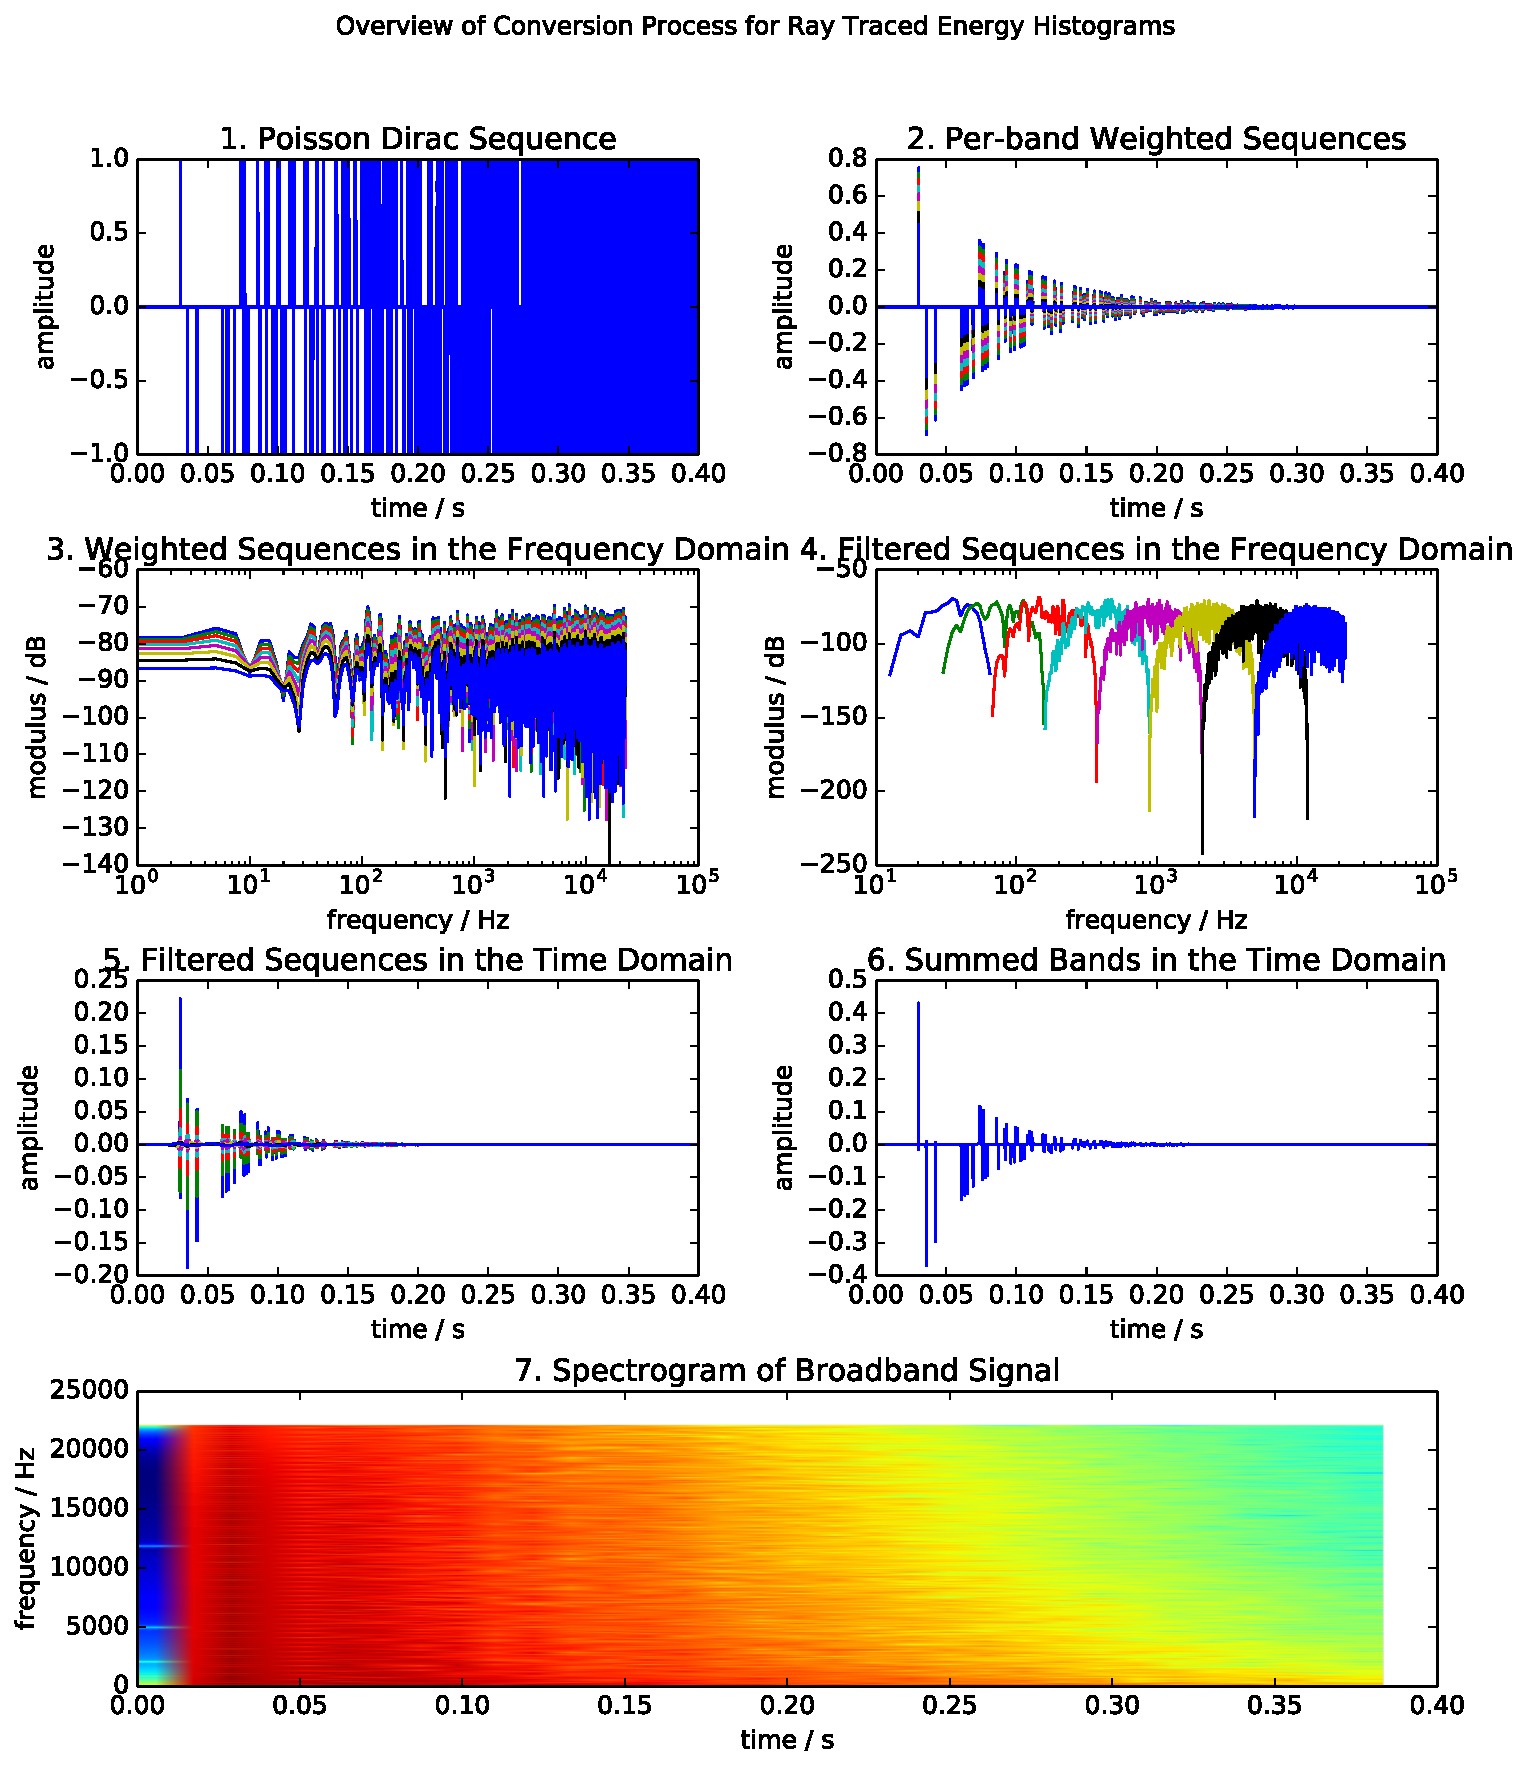
\includegraphics{images/raytrace_process.pdf}
\caption{Generating an audio-rate signal from multi-band ray tracing
energy histograms at a low sampling rate.\label{fig:raytrace_process}}
\end{figure}

\subsubsection{Generating a Noise
Signal}\label{generating-a-noise-signal}

First, a noise-like sequence of Dirac impulses is generated at
audio-rate. This sequence is designed to mimic the density of
reflections in an impulse response of a certain volume. Therefore it is
modelled as a temporal Poisson process which starts sparse, and with
increasing density of impulses over time. Specifically, the time between
one impulse event and the next is given by

\begin{enumerate}
\def\labelenumi{(\arabic{enumi})}
\setcounter{enumi}{9}
\tightlist
\item
  \[\Delta t_\text{event}(z) = \frac{\ln\frac{1}{z}}{\mu}\]
\end{enumerate}

where \(z\) is a uniformly distributed random number \(0 < z \leq 1\).
\(\mu\) here is the mean event occurrence, and is dependent upon the
current simulation time \(t\), the enclosure volume \(V\) and the speed
of sound \(c\):

\begin{enumerate}
\def\labelenumi{(\arabic{enumi})}
\setcounter{enumi}{10}
\tightlist
\item
  \[\mu = \frac{4\pi c^3 t^2}{V}\]
\end{enumerate}

It can be seen that the mean occurrence is proportional to the square of
the current time, producing an increase in event density over time. The
first event occurs at time \(t_0\):

\begin{enumerate}
\def\labelenumi{(\arabic{enumi})}
\setcounter{enumi}{11}
\tightlist
\item
  \[t_0=\sqrt[3]{\frac{2V\ln 2}{4\pi c^3}}\]
\end{enumerate}

The full-length noise signal is produced by repeatedly generating
inter-event times \(\Delta t_\text{event}\), and adding Dirac impulses
to a buffer, until the final event time is greater or equal to the time
of the final histogram interval. Dirac deltas falling on the latter half
of a sampling interval are taken to be negative-valued. The number of
Dirac deltas per sample is limited to one, and the value of \(\mu\) is
limited to a maximum of 10KHz, which has been shown to produce results
absent of obvious artefacts
{[}\protect\hyperlink{ref-heinzux5fbinauralux5f1993}{42}{]}.

\subsubsection{Weighting Noise
Sequences}\label{weighting-noise-sequences}

The noise sequence is duplicated, once for each frequency band. Then,
the noise sequence for each band is weighted according to that band's
histogram. This enveloping is not quite as simple as multiplying each
noise sample with the histogram entry at the corresponding time.
Instead, the enveloping process must conserve the energy level recorded
over each time step.

For each time interval in the histogram, the corresponding range of
samples in the noise sequence is found. If the output sample rate is
\(f_s\) and the histogram time step is \(\Delta t\), then the noise
sequence sample corresponding to histogram step \(h\) is
\(\lfloor h \cdot f_s \cdot \Delta t \rfloor\). The corrected energy
level for each histogram step is found by dividing the histogram energy
value by the sum of squared noise samples for that step. This is
converted to a corrected pressure level by \(P = \sqrt{Z_0 I}\), where
\(I\) is the corrected energy level, and \(Z_0\) is the acoustic
impedance of air. The weighting is now accomplished by multiplying each
noise sequence sample corresponding to this histogram step by the
corrected pressure level.

\subsubsection{Multi-band Filtering}\label{multi-band-filtering}

Now, we are left with a set of broadband signals, each with different
envelopes. The output signal is found by bandpass filtering each of
these signals, and then mixing them down.

The filter bank should have perfect reconstruction characteristics: a
signal passed through all filters in parallel and then summed should
have the same frequency response as the original signal. In the case
where all the materials in a scene have the same coefficients in all
bands, the input to each filter would be identical. Then, the expected
output would be this same as the input to any band (though band-passed
between the lower cutoff of the lowest band and the upper cutoff of the
highest band). Perfect-reconstruction filters maintain the correct
behaviour in this (unusual) case. It is especially important that the
bandpass filters are zero-phase, so that Dirac events in all bands are
in-phase, without group delay, after filtering. Finally, the filters
should have slow roll-off and no resonance, so that if adjacent bands
have very mismatched levels, there are no obvious filtering artefacts.

An efficient filtering method is to use a bank of
infinite-impulse-response filters. These filters are fast, and have low
memory requirements. They can also be made zero-phase when filtering is
offline, by running the filter forwards then backwards over the input
signal (though this causes filter roll-off to become twice as steep).
This was the initial method used in Wayverb: the filter bank was
constructed from second-order Linkwitz-Riley bandpass filters. This
method had two main drawbacks: the roll-off is limited to a minimum of
24 dB/octave
{[}\protect\hyperlink{ref-linkwitzux5factiveux5f1976}{43}{]}, which may
cause an obvious discontinuity in level in the final output; and the
forward-backward filtering method requires computing the initial filter
conditions in order to maintain perfect-reconstruction, which is
non-trivial to implement
{[}\protect\hyperlink{ref-gustafssonux5fdeterminingux5f1994}{44}{]}.

A better method, which allows for shallower filter roll-offs while
retaining perfect-reconstruction capabilities is to filter each band
directly in the frequency domain. The filtering of each signal is
accomplished by computing the signal's frequency-domain representation,
attenuating bins outside the passband, and then transforming the altered
spectrum back to the time domain. To ensure perfect reconstruction, and
to avoid artificial-sounding discontinuities in the spectrum, the filter
shape suggested in
{[}\protect\hyperlink{ref-antoniux5forthogonal-likeux5f2010}{45}{]} is
used. This paper suggests equations which describe the band-edge
magnitudes:

\begin{enumerate}
\def\labelenumi{(\arabic{enumi})}
\setcounter{enumi}{12}
\tightlist
\item
  \[
  G_\text{lower}(\omega_\text{edge} + p) = \sin^2\left(\frac{\pi}{2}\phi_l(p)\right), \\
  G_\text{upper}(\omega_\text{edge} + p) = \cos^2\left(\frac{\pi}{2}\phi_l(p)\right)
  \]
\end{enumerate}

Here, \(G\) is a function of frequency, \(\omega_\text{edge}\) is the
band-edge frequency, and \(p\) is the relative frequency of a nearby
frequency bin. The equations are computed for a range of values
\(p=P,\dots,P\) where \(P\) is the width of the crossover. The
definition of \(\phi_l(p), l \geq 0\) is recursive:

\begin{enumerate}
\def\labelenumi{(\arabic{enumi})}
\setcounter{enumi}{13}
\tightlist
\item
  \[
  \phi_l(p)=
  \begin{cases}
  \frac{1}{2}(p / P + 1), & l = 0 \\
  \sin(\frac{\pi}{2}\phi_{l-1}(p)), & \text{otherwise} 
  \end{cases}
  \]
\end{enumerate}

The variable \(l\) defines the steepness of the crossover, and is set to
0 in Wayverb, so that the transition between bands is as slow and smooth
as possible. The absolute width of the crossover is denoted by \(P\),
but it is more useful to specify the crossover width in terms of overlap
\(0 \leq o \leq 1\). Assuming logarithmically-spaced frequency bands,
spread over the range
\(\omega_\text{lowest}, \dots, \omega_\text{highest}\) where the edge
frequency of band \(i\) is defined as

\begin{enumerate}
\def\labelenumi{(\arabic{enumi})}
\setcounter{enumi}{14}
\tightlist
\item
  \[\omega_{\text{edge}_i}=\omega_\text{lowest}\left(\frac{\omega_\text{highest}}{\omega_\text{lowest}}^\frac{i}{N_\text{bands}}\right)\]
\end{enumerate}

the maximum width factor \(w\) is given by

\begin{enumerate}
\def\labelenumi{(\arabic{enumi})}
\setcounter{enumi}{15}
\tightlist
\item
  \[w=\frac{x-1}{x+1},
  x=\frac{\omega_\text{highest}}{\omega_\text{lowest}}^\frac{1}{N_\text{bands}}\]
\end{enumerate}

For \(\omega_\text{lowest}=20\text{Hz}\),
\(\omega_\text{highest}=20\text{KHz}\), and \(N_\text{bands}=8\),
\(w \approx 0.4068\). Then, the band edge width \(P\) can be defined in
terms of the overlap-amount \(o\), the frequency of this band edge
\(\omega_\text{edge}\), and the maximum allowable width factor \(w\):
\(P=\omega_\text{edge}ow\). Wayverb sets the overlap factor \(o=1\) to
ensure wide, natural-sounding crossovers.

The final broadband signal is found by summing together the weighted,
filtered noise sequences.

\chapter{Digital Waveguide Mesh}\label{digital-waveguide-mesh}

\section{Background}\label{background-2}

The \emph{digital waveguide mesh} (DWM) is one of several wave-based
simulation techniques. Each technique in this family is derived directly
from the wave equation, allowing them to inherently support wave
phenomena such as diffraction and interference. Wave effects such as
these have a great effect upon the low-frequency response of a room.
This means that at low frequencies wave-based methods are far more
accurate than geometric methods, which are not able to model wave
effects {[}\protect\hyperlink{ref-southernux5fspatialux5f2011}{1}{]}.

The drawback of wave-based methods is that their computational
complexity increases rapidly with the maximum output frequency, and with
the volume of the modelled space. A waveguide simulation of a space with
volume \(V\), at sampling frequency \(f_s\), will have a complexity of
\(O(V f_s^3)\). This means that, on current consumer hardware, it is not
feasible to compute a full-spectrum simulation using wave-based
techniques. The hybrid simulation method implemented in Wayverb aims to
optimise computation time, while retaining reasonable accuracy across
the spectrum, by combining wave-based methods with geometric methods.
Wave-based methods are used to calculate accurate low-frequency content,
while geometric methods estimate the higher frequency content, which is
less dependent upon wave effects.

There are, largely speaking, two main types of wave-based simulation
used for room acoustics: element methods, and finite difference methods.
The waveguide mesh is the latter, a simplified sub-class of the
\emph{finite-difference time-domain} (FDTD) technique. Although the DWM
and FDTD have converged over time, and are equivalent
{[}\protect\hyperlink{ref-smithux5fiiiux5fequivalenceux5f2004}{46}{]},
{[}\protect\hyperlink{ref-karjalainenux5fdigitalux5f2004}{47}{]}, their
histories are quite different. The DWM was designed to be efficient for
small-scale acoustic simulations in which the only quantity of interest
is pressure {[}\protect\hyperlink{ref-smithux5fphysicalux5f1992}{3}{]},
while FDTD is a more general technique designed for electromagnetic
simulation, in which the electric and magnetic fields are both of
interest {[}\protect\hyperlink{ref-bottsux5fintegratingux5f2013}{48}{]}.

\subsection{Method}\label{method}

The derivation of the waveguide mesh begins with the one-dimensional
\emph{digital waveguide}. A one-dimensional waveguide can exactly
describe the behaviour of a band-limited wave in one dimension. Such a
model is well-suited for predicting the behaviour of certain musical
instruments which use columns of air or vibrating strings to produce
sound. The model itself is based on d'Alembert's solution of the wave
equation in one dimension
{[}\protect\hyperlink{ref-shelleyux5fdiffuseux5f2007}{5}, p. 86{]}. The
displacement of a string \(y\) at time \(t\) and position \(x\) can be
written as

\begin{enumerate}
\def\labelenumi{(\arabic{enumi})}
\setcounter{enumi}{16}
\tightlist
\item
  \[y(t,x)=y_r\left(t-\frac{x}{c}\right) + y_l\left(t+\frac{x}{c}\right)\]
\end{enumerate}

where \(y_r\left(t-\frac{x}{c}\right)\) and
\(y_l\left(t+\frac{x}{c}\right)\) are the right- and left-going
travelling waves respectively, with speed \(c\)
{[}\protect\hyperlink{ref-smithux5fphysicalux5f1992}{3}{]}. The discrete
form of this equation is given in terms of constant time and space
divisions, \(T\) and \(X\) respectively:

\begin{enumerate}
\def\labelenumi{(\arabic{enumi})}
\setcounter{enumi}{17}
\tightlist
\item
  \[y(nT,mX) \buildrel \Delta \over = y^+(n-m) + y^-(n+m)\]
\end{enumerate}

where superscript \(+\) and \(-\) denote propagation to the right and
left respectively, and \(n\) and \(m\) are integers, used to index the
spatial and temporal sampling intervals
{[}\protect\hyperlink{ref-smithux5fiiiux5fequivalenceux5f2004}{46}{]}.

An implementation of these equations will take the form of two parallel
delay lines, which propagate wave components in opposite directions.
This is shown in the following
diagram\text{ (\ref{fig:one_d_waveguide})}. The ``output'' of the
simulation, that is, the physical displacement of the modelled string
over time, is found by adding the wave components in both delay lines at
a single point.

\begin{figure}[htbp]
\centering
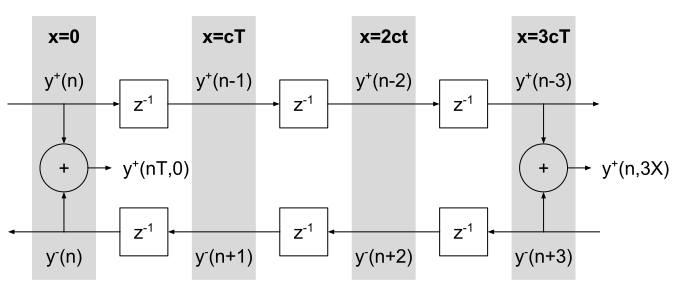
\includegraphics{images/one_d_waveguide.pdf}
\caption{Delay lines cause wave components to be propagated along the
``string'' over time. The total displacement of the string is found by
adding together values from the same point on each delay
line.\label{fig:one_d_waveguide}}
\end{figure}

Waveguides in higher dimensions can be created in a straightforward
manner, by connecting digital waveguide elements at a \emph{scattering
junction}. Wave components entering the junction are distributed amongst
the waveguide elements, preserving energy and power according to
Kirchoff's power conservation laws
{[}\protect\hyperlink{ref-shelleyux5fdiffuseux5f2007}{5}, p. 87{]}. The
sound pressure \(p_J\) at a lossless scattering junction \(J\) with
\(N\) connected elements or ``ports'' is the summed incoming components
of all connected elements:

\begin{enumerate}
\def\labelenumi{(\arabic{enumi})}
\setcounter{enumi}{18}
\tightlist
\item
  \[p_J=\frac{2\sum_{i=1}^{N}\frac{p_i^+}{Z_i}}{\sum_{i=1}^{N}\frac{1}{Z_i}}\]
\end{enumerate}

where \(p_i\) is the pressure in waveguide element \(i\) and \(Z_i\) is
its associated impedance. This simplifies, if all impedances are equal,
which is true for homogeneous media:

\begin{enumerate}
\def\labelenumi{(\arabic{enumi})}
\setcounter{enumi}{19}
\tightlist
\item
  \[p_J=\frac{2}{N}\sum_{i=1}^{N}p_i^+\]
\end{enumerate}

A \emph{digital waveguide mesh} is any configuration of
regularly-arranged \(N\)-port scattering junctions which are separated
by unit delay lines. In some literature, this specific type of mesh is
known as a \emph{W-DWM} because it operates in terms of ``W'' (wave)
variables.

The input into a scattering junction is equal to the output of a
neighbour junction at the previous time step. This fact allows the
waveguide mesh to alternatively be formulated directly in terms of the
pressure at each junction (assuming all junction impedances are equal)
{[}\protect\hyperlink{ref-beesonux5froomweaver:ux5f2004}{18}{]}:

\begin{enumerate}
\def\labelenumi{(\arabic{enumi})}
\setcounter{enumi}{20}
\tightlist
\item
  \[p_J(n)=\frac{2}{N}\sum_{i=1}^{N}p_i(n-1)-p_J(n-2)\]
\end{enumerate}

That is, the next pressure at a given node depends on the previous
pressure at that node, and the current pressure at surrounding nodes.
This alternative formulation operates on Kirchhoff variables, and is
therefore known as a \emph{K-DWM}. In the 1D case, the K-DWM and W-DWM
are computationally identical
{[}\protect\hyperlink{ref-smithux5fiiiux5fequivalenceux5f2004}{46}{]}.
In higher dimensions, they are equivalent only under certain
circumstances {[}\protect\hyperlink{ref-murphyux5facousticux5f2007}{49},
p. 5{]}.

The K-DWM is advantageous compared to the W-DWM for reasons of
efficiency. It requires less memory, and fewer calculations per node per
step than the W-DWM: experiments in
{[}\protect\hyperlink{ref-beesonux5froomweaver:ux5f2004}{18}{]} show
that the K-DWM is 200\% faster and uses 50\% of the memory of the
equivalent W-DWM. This is mainly to do with the number of values stored
per node. Each node in a K-DWM must store a ``current'' and a
``previous'' pressure value, whereas in a W-DWM each \emph{connection}
must store a value
{[}\protect\hyperlink{ref-karjalainenux5fdigitalux5f2004}{47}{]}. For
mesh layouts in which each node has many neighbours (see
\protect\hyperlink{mesh-topology}{Mesh Topology} below), the W-DWM can
require many times more memory. The K-DWM also requires one fewer
addition per node per step
{[}\protect\hyperlink{ref-shelleyux5fdiffuseux5f2007}{5}, p. 91{]}, so
will be slightly faster, all else being equal.

In the general case of an \(N\)-dimensional waveguide mesh, the spatial
and temporal sampling periods are related by the Courant number
\(\lambda\). The Courant criterion specifies the conditions required for
numerical stability of the simulation:

\begin{enumerate}
\def\labelenumi{(\arabic{enumi})}
\setcounter{enumi}{21}
\tightlist
\item
  \[\lambda=\frac{cT}{X} \leq \frac{1}{\sqrt{N}}\]
\end{enumerate}

The highest sampling rate and lowest error is achieved by setting the
Courant to its maximum value
{[}\protect\hyperlink{ref-sheafferux5ffdtdux2fk-dwmux5f2010}{50}{]}.
This is normally desirable, and so the inequality above can be
simplified:

\begin{enumerate}
\def\labelenumi{(\arabic{enumi})}
\setcounter{enumi}{22}
\tightlist
\item
  \[T=\frac{X}{c\sqrt{N}}\]
\end{enumerate}

A higher output sampling rate requires a smaller inter-nodal spacing and
therefore more modelled points per-unit-volume, which in turn requires
more memory and more calculations per time step.

An output signal created using a mesh with a sampling frequency
\(f_s = 1/T\) has a maximum available bandwidth which spans from DC to
the Nyquist frequency, \(0.5 \cdot f_s\). However, the \emph{valid}
bandwidth of the waveguide output is often considerably lower. For
example, the highest valid frequency in the rectilinear mesh is
\(0.196 \cdot f_s\). Detailed bandwidth information for other mesh
topologies is given in
{[}\protect\hyperlink{ref-kowalczykux5froomux5f2011}{35}{]}. The output
signal will contain high-frequency content above the maximum valid
frequency, however numerical dispersion in this region is so high that
the results are completely non-physical. To ensure that the output only
contains frequencies within the valid bandwidth, the invalid high
frequency content must be removed using a low-pass filter at the output.
Alternatively, the mesh may be excited using an input signal with no
frequency content above the maximum valid frequency.

\subsection{Strengths and Weaknesses of the
DWM}\label{strengths-and-weaknesses-of-the-dwm}

The main advantage of the DWM is its relative simplicity. The air in the
simulation is evenly divided into nodes. Each node has an associated
pressure, and also stores its previous pressure. The next pressure at a
node depends on its previous pressure, and the current pressures at its
neighbours. The simulation progresses by repeatedly updating all nodes,
and storing the change in pressure over time at some output nodes.

This simplicity presents an optimisation opportunity. Each node can be
updated completely independently, as long as all updates in one
time-step are completed before the next time-step begins. This means
that the updates can happen in parallel. In fact, with enough memory and
processing cores, the entire mesh could be updated in the time that it
takes to update a single node. The update method is also very simple,
only requiring some additions and a multiplication per node per step.
This kind of simple, parallel code lends itself to implementations on
graphics hardware, which is designed for running similar calculations
simultaneously over large inputs. \emph{Graphics processing units}
(GPUs) have best throughput when all threads execute the same
instruction, and when memory is accessed at consecutive addresses from
running threads. The K-DWM update equation has no branching, and has
consistent memory access patterns, which should allow for a very
efficient implementation for GPUs.

The greatest limitation of the DWM is \emph{dispersion error}. Unlike
waves in homogeneous physical media, the velocity of wave propagation in
the DWM depends on the direction of propagation, and also on the
frequency of the wave component. This leads to errors in the frequency
response of recorded signals, especially toward the upper limit of the
output bandwidth. The exact pattern of dispersion error is dependent
upon the topology of the mesh (topology is explained in
\protect\hyperlink{mesh-topology}{Mesh Topology} subsection), and can be
examined using \emph{Von Neumann} analysis
{[}\protect\hyperlink{ref-vanux5fduyneux5f3dux5f1996}{33}{]}. One
solution to the dispersion problem is to increase the sampling rate of
the mesh, moving the high-error area out of the region of interest. Of
course, this can quickly become very expensive, as the number of nodes,
and therefore memory usage and computation time is proportional to the
inverse cube of the sampling period. Another option is to use a mesh
topology designed to reduce both direction- and frequency-dependent
error, such as those presented in
{[}\protect\hyperlink{ref-kowalczykux5froomux5f2011}{35}{]}. One
interesting variation on this option is to reduce only
direction-dependent error, and then to compensate for
frequency-dependent error with a post-processing step, which is the
approach taken in
{[}\protect\hyperlink{ref-saviojaux5finterpolatedux5f2001}{11}{]}.
However, these mesh topologies with higher accuracy and isotropy require
relatively high numbers of calculations per node. The interpolated
schemes in {[}\protect\hyperlink{ref-kowalczykux5froomux5f2011}{35}{]}
require 27 additions and 4 multiplications per node, whereas a
tetrahedral mesh would require 5 additions and 1 multiplication. It is
clear that high-accuracy results will be very costly to compute,
whichever method is used.

\section{Design Choices}\label{design-choices}

\hypertarget{mesh-topology}{\subsection{Mesh
Topology}\label{mesh-topology}}

There is no single optimal implementation of the digital waveguide mesh.
Perhaps the most important decision is the mesh topology or
\emph{stencil} that will be used, and by extension the mesh update
equation. Here, the mesh topology refers to the pattern which is used to
distribute nodes throughout the modelled space. The choice of topology
will affect the accuracy, memory usage, calculation speed, and
implementation complexity of the final design. It must therefore be
chosen with care, in order to satisfy the constraints of the particular
application.

The simplest topology is rectilinear, in which nodes are laid out on the
vertices of a cubic grid, and each node has 6 direct neighbours. During
the mesh update, the pressure at each neighbour node must be checked in
order to calculate the next pressure at the current node. This is
straightforward to implement, as the nodes can be stored in memory in a
three-dimensional array, in which the array extents define the mesh
dimensions, and the array indices refer to the positions of individual
nodes. Other options for the topology include tetrahedral, octahedral,
and dodecahedral, in which nodes have 4, 8, and 12 neighbours
respectively, as shown in the following
figure\text{ (\ref{fig:topology})}.

\begin{figure}[htbp]
\centering
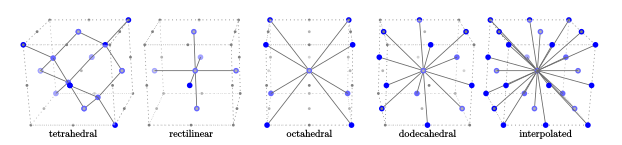
\includegraphics{images/topology.pdf}
\caption{Some of the most common mesh topologies. Black lines show
connections to nodes that will be checked during update. Note that the
tetrahedral topology is unique, in that nodes can have two different
orientations.\label{fig:topology}}
\end{figure}

The accuracy may be increased by overlaying or ``superposing''
rectilinear, octahedral, and dodecahedral schemes together, as all nodes
are oriented uniformly, and have cubic tessellation. Such schemes are
known as \emph{interpolated}, and in these schemes each node has 26
neighbours. The rectilinear, octahedral, dodecahedral, and interpolated
schemes may additionally all be represented by a single ``unified''
update equation, described in
{[}\protect\hyperlink{ref-kowalczykux5froomux5f2011}{35}{]}. In this
respect the tetrahedral scheme is unique, requiring a dedicated update
method. This is because the node connection in a tetrahedral mesh may be
oriented in either of two directions, effectively requiring two update
equations instead of one.

If the primary concern is speed rather than accuracy, a scheme with
fewer neighbour nodes should be used, as the number of calculations per
node is proportional to the number of neighbours
{[}\protect\hyperlink{ref-camposux5fcomputationalux5f2005}{8}{]}. The
tetrahedral mesh has fewest neighbours per node, and also has the lowest
density. That is, it requires the fewest nodes to fill a volume at any
given sampling rate. Fewer nodes to update means fewer calculations, and
a faster overall simulation. Lower density meshes also require less
storage, so the tetrahedral scheme is the most time and memory
efficient.

To optimise for accuracy, it appears that there are two possible
approaches: The first option is to use an interpolated scheme, which is
relatively inefficient in terms of time and space requirements, but
which is most accurate for any given sampling rate. The second option is
to use a tetrahedral mesh, which is inaccurate but the most time- and
space-efficient, and to oversample until the required accuracy is
achieved. Unfortunately, there is no prior research comparing the
accuracy and efficiency of the tetrahedral topology against interpolated
schemes. Due to time constraints, this could not be investigated as part
of the Wayverb project (implementation and numerical analysis of mesh
topologies is not trivial). It was, however, noted that the tetrahedral
mesh is the more flexible of the two approaches. That is, when accuracy
is not important, the tetrahedral mesh will always be most efficient,
but it can be made more accurate by oversampling. On the other hand, the
interpolated schemes cannot be tuned to produce less accurate results
quickly - they will always be accurate but inefficient. For these
reasons, the tetrahedral mesh was initially chosen for use in Wayverb.

The tetrahedral mesh was implemented during within the first two months
of the project, with support for microphone modelling. When it came to
implementing frequency dependent boundary conditions, no prior research
could be found discussing boundary implementations in a tetrahedral
topology. As noted in the conclusion of
{[}\protect\hyperlink{ref-kowalczykux5froomux5f2011}{35}{]}:

\begin{quote}
One aspect that has not been dealt with in this paper, and could be of
interest for future research, is the comparison of the identified
schemes with the tetrahedral topology\ldots{} However, the applicability
of the tetrahedral stencil to room acoustic simulations is debatable due
to the nontrivial formulation of boundary conditions for complex room
shapes.
\end{quote}

The design of a new boundary formulation is outside the scope of this
research, which was primarily concerned with the implementation of
existing techniques rather than the derivation of new ones. Instead, the
standard leapfrog (rectilinear) scheme was adopted at this point. Most
of the tetrahedral code had to be rewritten, as the update schemes are
very different (tetrahedral nodes have two possible update equations
depending on node orientation), and the memory layout and indexing
methods are more involved. The new scheme is much simpler than the
tetrahedral mesh, and was quick to implement.

The rectilinear mesh uses the same cubic tessellation as the more
complex topologies mentioned earlier, so in the future the update
equation could conceivably be replaced with a more accurate
``interpolated'' alternative. Such a scheme would be more suitable than
the rectilinear mesh for simulations where high accuracy is required.
The conversion would only require changes to the update equations (and
would complicate the boundary modelling code), but would be more
straightforward than the move from the tetrahedral to the rectilinear
topology. Due to time constraints, this was not possible during the
project, meaning that the waveguide in Wayverb is not the most optimal
in terms of accuracy \emph{or} speed. Interpolated meshes are more
accurate, and tetrahedral meshes are faster, although the rectilinear
mesh is the fastest mesh with a cubic stencil. Instead, Wayverb's
waveguide was optimised for ease and speed of implementation. Use of a
more suitable mesh topology would be a sensible starting point for
future development work on the project.

\subsection{Source Excitation Method}\label{source-excitation-method}

Input and output methods for the digital waveguide mesh are
superficially simple. The waveguide mesh is a physical model, and so it
is easy to draw an analogy between the waveguide process, and the
process of recording a physical impulse response. Typically, for
physical spaces, a speaker plays a signal at some location within the
space, and a microphone reads the change in air pressure over time at
another point in the space. The impulse response is found by
deconvolving the input signal from the recorded signal. The analogue of
this process within the waveguide mesh is to excite the mesh at one
node, and to record the pressure at some output node at each time step,
which is then deconvolved as before. Recording node pressures is simple,
and deconvolution is a well-known technique. Injecting a source signal,
however, requires careful engineering in order to maintain the physical
plausibility and numerical robustness of the model. Source design has
two main concerns: the method that is used to add the signal into the
mesh, and the signal that is injected.

\subsubsection{Input Node Update Method}\label{input-node-update-method}

Firstly, the input signal may be injected at a single node, or
distributed across several
{[}\protect\hyperlink{ref-jeongux5fsourceux5f2012}{51}{]}. It is
complicated to calculate an appropriate distributed signal
{[}\protect\hyperlink{ref-sakamotoux5fphase-errorux5f2007}{52}{]}, and
so single-node sources are more common in the literature
{[}\protect\hyperlink{ref-jeongux5fsourceux5f2012}{51}{]},
{[}\protect\hyperlink{ref-lamux5ftimeux5f2012}{53}{]}--{[}\protect\hyperlink{ref-dimitrijevicux5foptimizationux5f2015}{56}{]}.

There are two main options for updating the source node with the input
signal. The first method, known as a \emph{hard source}, simply
overwrites the pressure value at the source node with that of the input
signal. Hard sources are simple to implement, and ideally couple the
input signal to the mesh, but also scatter any incident wave-fronts
{[}\protect\hyperlink{ref-schneiderux5fimplementationux5f1998}{57}{]}.
Although the initially radiated field is optimal, this spurious
scattering is an undesirable artefact. Furthermore, the abrupt pressure
discontinuity introduced by the hard source can cause more artefacts
through the accumulation of numerical errors. For these reasons, hard
sources are generally unsuitable for high-accuracy simulations.

The second method, the \emph{soft source}, instead adds or superimposes
the input signal on the standard mesh update equation. Soft sources obey
the mesh update equations, and so do not suffer from the scattering
problem. However, they do not couple the input signal to the mesh, so
that the radiated wave front does not resemble the input signal. For
input signals with DC components, soft sources can lead to
\emph{solution-growth}, in which the DC level of the entire simulation
increases exponentially over time. This is not to do with numerical
error or stability. Rather, the DC component suggests that the input
signal is of infinite length, and that the source continues to create
volume velocity for the duration of the simulation
{[}\protect\hyperlink{ref-sheafferux5fphysically-constrainedux5f2012}{58}{]}.
That is, the model is valid, but it is being used to model a
physically-implausible situation. Solution-growth is unacceptable for
modelling purposes. In all cases it creates an increasing DC component
which is difficult to remove from the output. It also leads to a loss of
precision in floating-point simulations, as intervals between
floating-point numbers are larger for higher-magnitude numbers. The
low-magnitude content of interest cannot be specified with high
precision when it is superimposed on a high-magnitude DC component. In
the worst case, the DC component will build up so much that the
numerical representation ``overflows'', placing an upper bound on the
duration of the simulation. Some of the drawbacks of the soft source can
be alleviated by carefully constructing the input signal, which will be
discussed later.

Solution growth is not seen in hard source models, because the source
node pressure is replaced by that of the input function. Therefore, at
the source node, there is no addition of DC level. Unfortunately,
rarefaction cannot occur at the source node, which can cause
low-frequency oscillations instead. These oscillations are easier to
remove than an increasing DC offset, and have less impact on precision.

A special case of the soft source is the \emph{transparent source},
described in
{[}\protect\hyperlink{ref-schneiderux5fimplementationux5f1998}{57}{]}.
This method is the same as the soft source, but additionally subtracts
the convolution of the mesh impulse response with the input signal from
the input node. The resulting wave-front has the same characteristics as
that produced by a hard source, with the additional benefit that
incident wave-fronts are not scattered. The drawback of this technique
is that the mesh impulse-response must be precomputed before the
simulation can begin, which is achieved by running a separate (costly)
waveguide mesh simulation. Once found, the mesh response can be used for
any other simulation sharing the same mesh topology. Although the
transparent source is complex to set up, its characteristics seem
perfect. It behaves as if the input signal is perfectly coupled to the
mesh, and there is no scattering problem. However, it retains the
solution-growth issue of the general soft source.

The hard and soft source methods can be combined, in order to benefit
from the characteristics of both methods. A \emph{time-limited pulse}
method is introduced in
{[}\protect\hyperlink{ref-jeongux5fsourceux5f2012}{51}{]}, in which the
source node starts as a hard source, and reverts to a soft source after
a certain period of time has elapsed. The input signal is ideally
coupled to the mesh for its duration, but thereafter the mesh can update
as usual. As long as the source is positioned away from reflective
boundaries, this solves the scattering issue. However, if the source is
near to a reflective boundary, reflected wave-fronts might reach the
source node before it has reverted to the standard update equation,
scattering them. This input scheme has similar performance to the
transparent source, with much reduced complexity, but it also shares a
major drawback. If the input signal has a DC component, the time-limited
hard source can still cause solution-growth
{[}\protect\hyperlink{ref-sheafferux5fphysically-constrainedux5f2012}{58}{]}.
In addition, if the nodes next to the source are not zero when the
update equation switches from hard to soft, the pressure discontinuity
introduced may introduce error which will propagate for the remainder of
the simulation
{[}\protect\hyperlink{ref-sheafferux5fphysicalux5f2014}{54}{]}.

On balance, it seems as though the transparent source is the optimum
input method. Once the mesh impulse response has been computed, the
update method itself is simple to implement, and does not carry any
performance penalties. The only disadvantage is that the input function
must be carefully designed to have no DC component, to avoid
solution-growth. Unfortunately, overcoming this weakness is somewhat
difficult, as will be shown in the following subsection.

\subsubsection{Input Signal}\label{input-signal}

Of course, the input signal must be bounded in time, so that the
simulation can end. The shorter the input signal, the fewer simulation
steps must be computed, so shorter inputs are more efficient. If a
single-sample Dirac-delta is used, all frequencies in the output
bandwidth will be excited equally, and the output will not require
deconvolution, which is another computational saving. It is plain that a
short impulsive input is desirable in terms of efficiency.
Unfortunately, impulsive signals have a DC component, which can cause
solution-growth with soft, particularly transparent, sources.

The constraints of the input signal are, therefore, as follows: The
signal shall have no DC component. It shall be as short as possible, to
minimise the simulation time. It shall have a wide and flat passband, to
increase the accuracy of the deconvolution. The time-compactness and
bandwidth constraints are mutually exclusive, so in practice the input
length must be chosen to balance bandwidth and calculation time.

Particular constraints of source signals are presented in greater detail
in {[}\protect\hyperlink{ref-sheafferux5fphysicalux5f2014}{54}{]}, which
puts forward an additional constraint, known as the
\emph{differentiation constraint}: The input signal shall be equal to
the first time derivative of fluid emergence. Fluid emergence should
start and end at zero, which in turn enforces a null DC component.

Some particular possibilities for the input signal are the
\emph{sine-modulated Gaussian pulse} {[}jeong\_source\_2012{]}, and the
\emph{differentiated Gaussian pulse} and \emph{Ricker wavelet}
{[}\protect\hyperlink{ref-sheafferux5fphysicalux5f2014}{54}{]}. All of
these signals satisfy the differentiation constraint and the length
constraint. However, they all have non-flat pass-bands, as shown in the
following figure\text{
(\ref{fig:input_signal_info})}. A final option is the \emph{physically
constrained source} (PCS) model presented in
{[}\protect\hyperlink{ref-sheafferux5fphysicalux5f2014}{54}{]}. This
method can be used to create input signals with pass-bands much flatter
than those of the more conventional pulse and wavelet signals. PCS
signals obey the differentiation constraint, have wide and flat
passbands, and are short in time. They use soft-source injection, so
will not cause scattering artefacts, and as they have no DC component,
they should not introduce solution-growth. A PCS input signal seems like
and obvious choice for this application.

\begin{figure}[htbp]
\centering
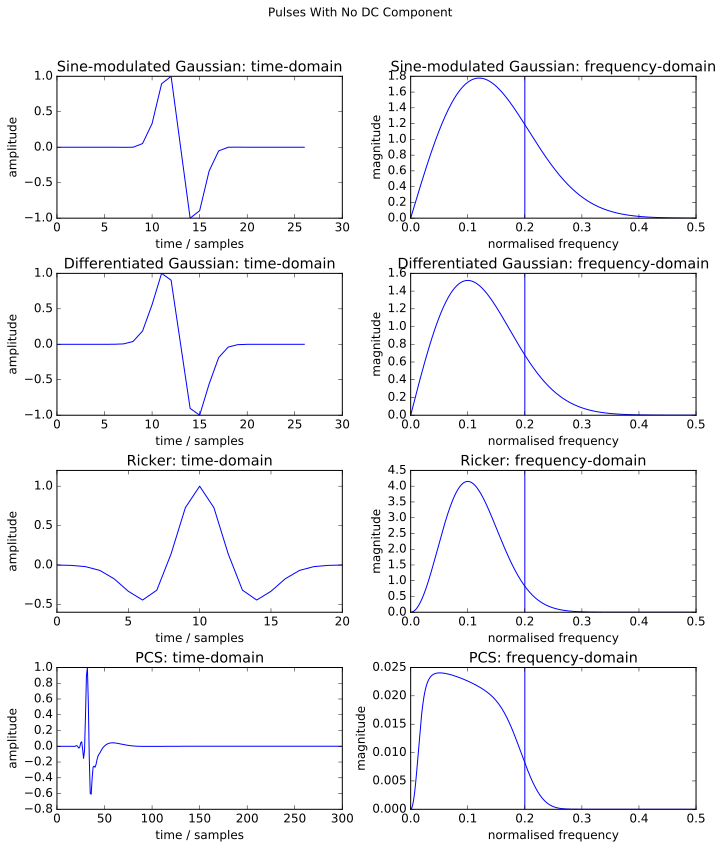
\includegraphics{images/kernel_properties.pdf}
\caption{The time-domain and frequency-domain responses of some signals
commonly used as FDTD excitations. All signals are shown with an upper
cutoff of \(0.2f_s\). The pulse signals have their centre frequencies
set to \(0.1f_s\). The PCS signal shown has a sampling rate of 10KHz, a
mass of 25g, a low cutoff of 100Hz, and a Q of 0.7. It \emph{includes}
the injection filter, which means the signal shown could be injected
like a soft source. \label{fig:input_signal_info}}
\end{figure}

A test was devised to ensure that the source injection method did not
cause solution-growth. A standard rectilinear waveguide mesh with a
sampling frequency of 10KHz was set up within a cuboid room, measuring
\(5.56 \times 3.97 \times 2.81\) metres. A source was placed at (4.8,
2.18, 2.12), and a receiver at (4.7, 2.08, 2.02). The walls of the room
were set to have a uniform broadband absorption of 0.006 (see the
\href{\%7B\%7B\%20site.baseurl\%7D\%7D\%7B\%\%20link\%20boundary.md\%20\%\%7D}{Boundary
Modelling} section). ``Transparent'' input signals were created from a
differentiated Gaussian pulse, a sine-modulated Gaussian pulse, and a
Ricker wavelet, all of which were set to a centre frequency of 0.05
\(f_s\). A physically-constrained source signal was also generated,
using parameters suggested in section V of
{[}\protect\hyperlink{ref-sheafferux5fphysicalux5f2014}{54}{]}: a
max-flat finite-impulse-response pulse-shaping filter kernel with 16
taps and centre frequency of 0.075 \(f_s\) and magnitude 250μN was
generated; it was passed through a mechanical shaping filter with radius
5cm, mass 25g, lower cutoff 100Hz, and resonance 0.7; then this signal
was passed through an infinite-impulse-response \emph{injection filter},
and used as a soft source. (These parameters are reproduced here to
ensure that the test is repeatable, but a full discussion of their
meaning is beyond the scope of this paper. The interested reader is
directed to
{[}\protect\hyperlink{ref-sheafferux5fphysicalux5f2014}{54}{]} or to the
implementation of the physically-constrained source in the Wayverb
repository.) Finally, the simulation was run for around 85000 steps
(less than the expected Sabine RT60 of the room) with each of the four
sources, and the response at the receiver was recorded.

The results of the experiment are shown in the following figure\text{
(\ref{fig:solution_growth_results})}. The response of a transparent
Dirac source (which has a strong DC component) is also shown. Solution
growth can be seen in all the outputs. However, the magnitude of growth
is different depending on the input signal. As expected, the Dirac
signal exhibits the largest rate of growth, followed by the
differentiated Gaussian, sine-modulated Gaussian, Ricker wavelet, and
finally the PCS signal. All the sources with no DC component show
significantly less solution-growth than the transparent Dirac source.
The PCS has a much lower rate of growth than the alternatives. However,
all inputs \emph{do} show the effects of solution-growth.

\begin{figure}[htbp]
\centering
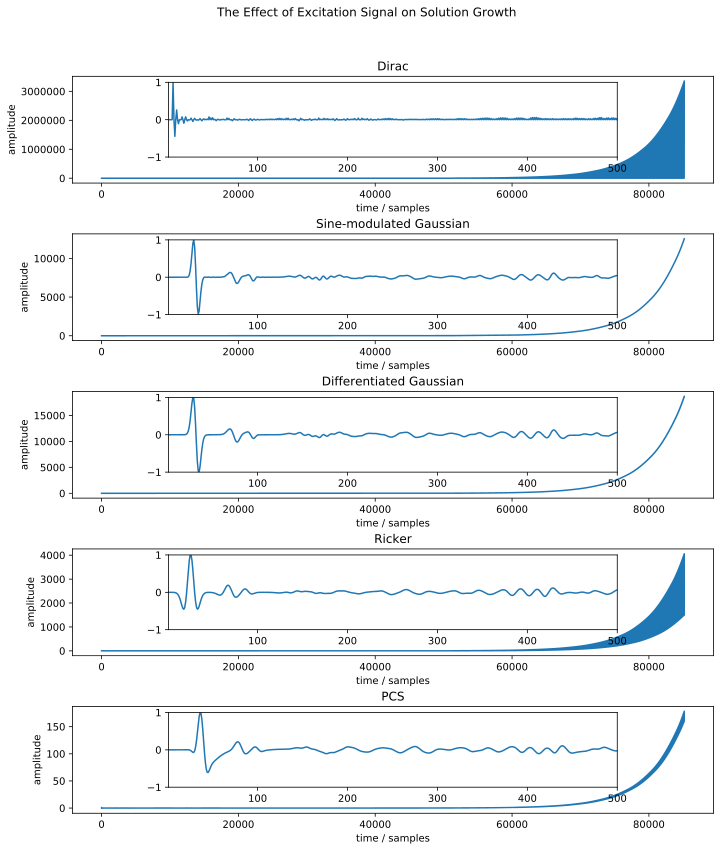
\includegraphics{images/solution_growth.pdf}
\caption{Solution growth in the waveguide mesh with a selection of
different inputs. Results are normalized so that the initial wave-fronts
have the same magnitude. The overlays show the initial 500 samples of
the response on the same scale, highlighting the different shapes of the
excitation signals. The full signals are shown behind, with
\emph{different} amplitude scales. \label{fig:solution_growth_results}}
\end{figure}

The solution-growth seen here only becomes prominent towards the end of
the simulation, after around 60000 steps. However, papers which propose
countermeasures to the solution-growth problem generally only test their
solutions up to 15000 steps or so
{[}\protect\hyperlink{ref-jeongux5fsourceux5f2012}{51}{]},
{[}\protect\hyperlink{ref-sheafferux5fphysicalux5f2014}{54}{]},
{[}\protect\hyperlink{ref-sheafferux5fphysically-constrainedux5f2012}{58}{]}.
The results of testing the solution in
{[}\protect\hyperlink{ref-dimitrijevicux5foptimizationux5f2015}{56}{]}
are not even presented. It is entirely possible that these input methods
have not been tested in such a long simulation before.

The reason for the solution-growth is not clear. In general, the problem
is caused by repeated superposition of the DC level, which is reflected
from boundaries. The waveguide has no inherent way of removing DC, so
\emph{any} small DC component will accumulate over time. If the original
signal does not have a DC component, then the DC is being added from
elsewhere. The most likely origin is numerical error in the waveguide
mesh. The experiment above uses 32-bit single-precision floating-point
to represent the pressure of mesh nodes, which is necessary because
using double-precision would double the memory usage and halve the
computational throughput. It is possible that error in these
single-precision calculations manifests as a tiny DC component, which
then multiplies as the simulation progresses.

Whatever the reason, it is clear that using a soft source generally
causes a DC offset to accumulate, even when the input signal has no DC
component. Soft sources may be suitable for shorter simulations.
However, without running the simulation, it is impossible to know how
much DC will accumulate, and whether or not it will remain within
acceptable bounds. Therefore, in general, current forms of the soft
source are not appropriate for arbitrary room simulation.

As an alternative to a soft source, Wayverb currently uses a hard source
with a Dirac impulse as its input method. Though this still causes
low-frequency error
{[}\protect\hyperlink{ref-sheafferux5fphysicalux5f2014}{54}{]}, this
error manifests as an oscillation rather than an exponential growth. The
oscillation tends to be below the audible range, and therefore can be
removed without affecting the perceived quality of the simulation. This
removal is achieved with no phase modifications by transforming the
signal into the frequency domain, smoothly attenuating the lowest
frequencies, and then converting back to the time domain. This is the
same filtering process used throughout Wayverb, described in detail in
the
\href{\%7B\%7B\%20site.baseurl\%20\%7D\%7D\%7B\%\%20link\%20ray_tracer.md\%20\%\%7D}{Ray
Tracer} section. The main drawback of the hard source is its scattering
characteristic. Though undesirable, this behaviour has a physical
analogue: in a physical recording, reflected wave-fronts would be
scattered from the speaker cabinet or starter pistol used to excite the
space.

The creation of soft sources which do not cause solution growth is an
important area for future research. Code for modelling soft sources
remains in the Wayverb repository, to ease further development work in
this area. If a better excitation method is discovered, it will be easy
to replace the current source model with the improved one.

\section{Implementation}\label{implementation-2}

Here, the final waveguide, as implemented in Wayverb, is described. Room
acoustics papers tend not to discuss the set-up process for 3D waveguide
meshes, so this process will be described in detail here.

\subsection{Inner and Outer Nodes}\label{inner-and-outer-nodes}

Prerequisites for the simulation are: a 3D scene, made up of triangles,
each of which has multi-band absorption coefficients; a source and
receiver position within the scene; the speed of sound \(c\) and
acoustic impedance of air \(Z_0\), and the sampling frequency of the
mesh \(f_s\). This sampling frequency may be derived from a maximum
cutoff frequency and an oversampling coefficient.

The first step is to calculate the position of each node in the mesh.
The inter-nodal spacing \(X\) (that is, the spatial sampling period) is
given by

\begin{enumerate}
\def\labelenumi{(\arabic{enumi})}
\setcounter{enumi}{23}
\tightlist
\item
  \[X=\frac{c}{f_s\lambda} = \frac{c\sqrt{3}}{f_s}\]
\end{enumerate}

where \(\lambda\) is the Courant number, set to its maximum stable
value. Now, the axis-aligned bounding box of the scene is found, and
padded to exact multiples of the grid spacing along all axes. The exact
padding is chosen so that one node will fall exactly at the receiver
position, and so that there is room for an ``outer layer'' at least two
nodes deep around the scene. This outer padding is to accommodate for
boundary nodes, which will always be quantised to positions just outside
the modelled enclosure. If the new padded bounding box has minimum and
maximum corners at 3D points \(c_0\) and \(c_1\), then the position of
the node with integer indices \((i, j, k)\) is given by
\(c_0 + X(i, j, k)\). The number of nodes in each direction is given by
\(\frac{c_1 - c_0}{X}\). The actual node positions are never computed
and stored, because this would take a lot of memory. Instead, because
the calculation is so cheap, they are recomputed from the node index,
bounding box, and mesh spacing whenever they are needed.

Each node position must be checked, to determine whether it falls inside
or outside the scene. The algorithm for checking whether a node is
inside or outside is conceptually very simple: Follow a ray from the
node position in a random direction chosen from a uniform distribution,
until it leaves the scene bounding box. If the ray intersects with an
odd number of surfaces, the point is inside; otherwise it is outside.
There is an important special case to consider. Floating-point math is
imprecise, so rays which ``graze'' the edge of a triangle may be falsely
reported as intersecting or not-intersecting. This is especially
problematic if the ray intersects an edge between two triangles, in
which case zero, one, or two intersections may be registered. To solve
this problem, the intersection test can return three states instead of
two (``uncertain'' as well as ``definite intersection'' and ``definitely
no intersection''). If the ray grazes any triangle, then ``uncertain''
is returned, and a new random ray is fired. The process then repeats
until a ray with no grazing intersections is found. Note that this
algorithm relies on ray-casting, which means that it can be accelerated
using the voxel-based method discussed in the
\href{\%7B\%7B\%20site.baseurl\%20\%7D\%7D\%7B\%\%20link\%20image_source.md\%20\%\%7D}{Image
Source} section. All tests are carried out in parallel on the GPU, and
the results are stored.

\subsection{Boundary Node
Classification}\label{boundary-node-classification}

Now the inner nodes are known. However, the remaining nodes are not all
``outside'' the simulation: some are ``boundary'' nodes (see
\href{\%7B\%7B\%20site.baseurl\%20\%7D\%7D\%7B\%\%20link\%20boundary.md\%20\%\%7D}{Boundary
Modelling}). These boundary nodes must be found and classified.

Boundary nodes fall into three main categories, shown in the following
diagram\text{ (\ref{fig:boundary_types})}:

\begin{itemize}
\tightlist
\item
  \textbf{1D} nodes are situated directly adjacent to a single inner
  node in one of the six axial directions.
\item
  \textbf{2D} nodes are next to a single inner node in one of the twelve
  on-axis diagonal directions.
\item
  \textbf{3D} nodes are next to a single inner node in one of the eight
  off-axis diagonal directions.
\end{itemize}

\begin{figure}[htbp]
\centering
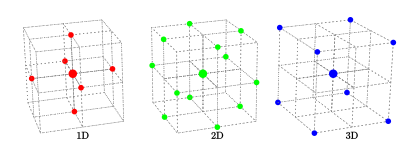
\includegraphics{images/boundary_types.pdf}
\caption{A given node (represented by a large dot) is a boundary node if
it is \emph{not} an inner node, but there is an adjacent inner node at
one of the locations shown by smaller dots.\label{fig:boundary_types}}
\end{figure}

There is also a fourth category, known as \emph{re-entrant} nodes, which
are adjacent to two or more inner nodes. These nodes are special, in
that they fall outside the enclosure (like boundary nodes) but are
updated using the standard inner node equation. Re-entrant nodes are
generally found on corners which face ``into'' the enclosed space.

The classification proceeds as follows: For a given node, if it is
inside, return. Otherwise, check the node's six axial neighbours. If one
neighbour is inside, the node is a 1D boundary; if two neighbours are
inside, the node is re-entrant; if no neighbours are inside the node
remains unclassified. If the node is unclassified, check the twelve
on-axis diagonal neighbours. If one neighbour is inside, the node is a
2D boundary; if two neighbours are inside, the node is re-entrant; if no
neighbours are inside the node is still unclassified. Finally, check the
eight off-axis diagonal neighbours. If one neighbour is inside, the node
is a 3D boundary; if two neighbours are inside, the node is re-entrant;
if no neighbours are inside, the node is an ``outer'' node and can be
ignored for the remainder of the simulation. This classification process
can of course be run in parallel on the GPU.

The classification is a little too involved to recompute regularly, so
the results of the classification are cached. Each node stores its
characteristics into a integer which behaves as a bitfield, allowing the
characteristics to be stored in a compact form. Bits have the following
significance:

\begin{Shaded}
\begin{Highlighting}[]
\KeywordTok{typedef} \KeywordTok{enum} \NormalTok{: cl_int \{}
    \NormalTok{id_none = }\DecValTok{0}\NormalTok{,}
    \NormalTok{id_inside = }\DecValTok{1} \NormalTok{<< }\DecValTok{0}\NormalTok{,}
    \NormalTok{id_nx = }\DecValTok{1} \NormalTok{<< }\DecValTok{1}\NormalTok{,}
    \NormalTok{id_px = }\DecValTok{1} \NormalTok{<< }\DecValTok{2}\NormalTok{,}
    \NormalTok{id_ny = }\DecValTok{1} \NormalTok{<< }\DecValTok{3}\NormalTok{,}
    \NormalTok{id_py = }\DecValTok{1} \NormalTok{<< }\DecValTok{4}\NormalTok{,}
    \NormalTok{id_nz = }\DecValTok{1} \NormalTok{<< }\DecValTok{5}\NormalTok{,}
    \NormalTok{id_pz = }\DecValTok{1} \NormalTok{<< }\DecValTok{6}\NormalTok{,}
    \NormalTok{id_reentrant = }\DecValTok{1} \NormalTok{<< }\DecValTok{7}\NormalTok{,}
\NormalTok{\} node_type;}
\end{Highlighting}
\end{Shaded}

The descriptor field for an inner node will be set to
\texttt{id\_inside}, and for a re-entrant node will be set to
\texttt{id\_reentrant}. Boundary nodes are described by setting bits
equal to the direction of the adjacent inner node. A 1D node with an
inner neighbour in the negative-x direction will have the descriptor
\texttt{id\_nx}, a 2D node with an inner neighbour on the positive-y-z
diagonal will have the descriptor \texttt{id\_py\ \textbar{}\ id\_pz}
(where \texttt{\textbar{}} is a bitwise-or operator), and a 3D node with
an inner neighbour on the positive-x, negative-y, positive-z diagonal
will have the descriptor
\texttt{id\_px\ \textbar{}\ id\_ny\ \textbar{}\ id\_pz}.

\subsection{Boundary Behaviour and
Materials}\label{boundary-behaviour-and-materials}

Each boundary node behaves as if it has an internal IIR filter. More
precisely, 1D nodes have a single internal IIR filter, while 2D and 3D
nodes have two and three internal filters respectively. To operate,
these filters must reference filter coefficients which approximate the
wall behaviour, and must also have dedicated storage for their filter
delay lines.

First, the numbers of 1D, 2D, and 3D boundary nodes are counted. An
array of single-filter delay lines is created, containing one delay line
for each 1D node. The same is done for the 2D and 3D nodes, but each
element in these arrays has storage for two and three filter delay lines
respectively. Now, each boundary node is given a unique index which is
used to reference an element in its corresponding filter memory array.
These unique indices are simple to compute: for each node in the
simulation, if it is 1D (or 2D, or 3D), increment a counter, and use the
counter value as the unique index.

For each material in the scene, the Yule-Walker method is used to
generate an IIR filter representing that material, resulting in an array
of IIR filter coefficients. Each filter delay line is paired with an
index field, which allows it to reference the filter coefficients which
should be used when updating the filter.

The final step is to find which filter coefficients should be linked to
which filter delay line. For 1D boundaries, the process is as follows:
find the closest triangle to the node; find the material index of that
triangle; get the node's filter data entry; set the coefficient index
field to be equal to the closest triangle's material index. For 2D
boundaries, adjacent 1D boundary nodes are checked, and their filter
coefficient indices are used, which saves running further
closest-triangle tests. For 3D boundaries, adjacent 1D \emph{and} 2D
nodes are checked.

\begin{figure}[htbp]
\centering
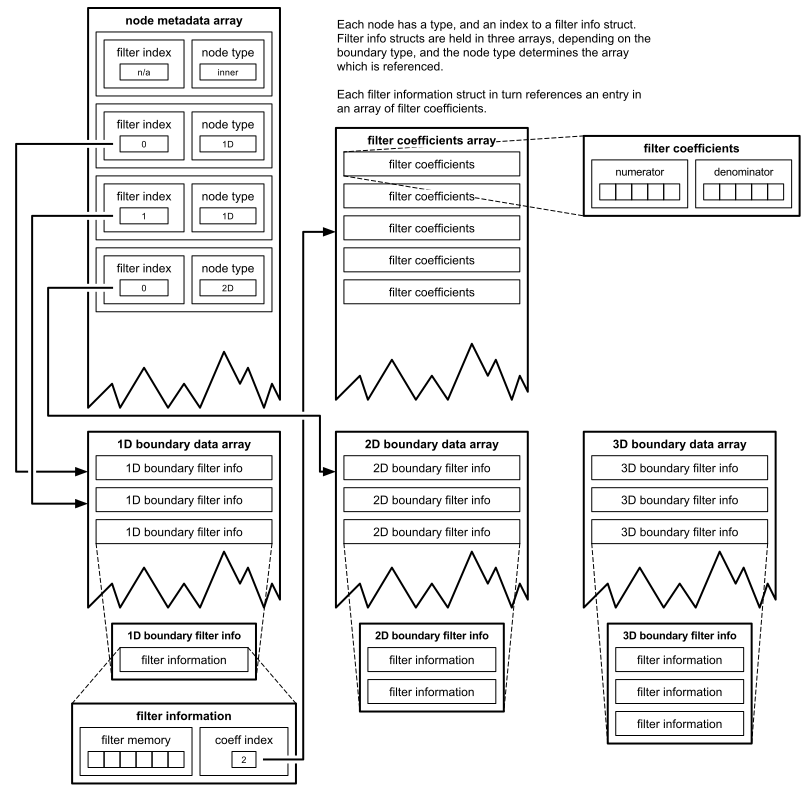
\includegraphics{images/memory_layout.pdf}
\caption{Efficient memory usage is important in large-scale simulations
such as those conducted by Wayverb. The waveguide storage scheme aims to
minimise redundant duplication of data.\label{fig:memory_layout}}
\end{figure}

\subsection{Running the Simulation}\label{running-the-simulation}

With node properties and boundary information set up, all that remains
is to run the simulation itself. Two arrays of floating-point numbers
are allocated, with length equal to the number of nodes in the
simulation. These arrays represent the current and previous pressures at
each node. The simulation is then run for a certain number of steps. In
Wayverb the simulation length is found using the time of the final
ray-traced histogram bin, divided by the mesh sampling frequency. In
most cases this will lead to a sufficiently accurate duration estimate.
However, in very large or irregularly-shaped rooms where few
ray-receiver intersections are recorded, this may lead the waveguide
simulation time to be underestimated. In this scenario, the simulation
time can be found with greater accuracy by increasing the number of
rays.

During a single step of the simulation, each node is updated. These
updates occur in parallel, using the GPU. The ``descriptor'' field of
each node is checked, and if it is \texttt{id\_none} then the node is
ignored. If the descriptor is \texttt{id\_inside} or
\texttt{id\_reentrant} then the node is updated like a normal air node;
that is, the ``next'' pressure of the node is equal to the sum of
current axially-adjacent pressures divided by three, minus the previous
pressure of the node. This is shown in the following equation, where
\(i\), \(j\), and \(k\) are spatial indices on the \(x\), \(y\) and
\(z\) axes respectively, and \(n\) is a time index.

\begin{enumerate}
\def\labelenumi{(\arabic{enumi})}
\setcounter{enumi}{24}
\tightlist
\item
  \[p_{i,j,k}^{n+1} = \frac{1}{3}(p_{i-1,j,k}^n + p_{i+1,j,k}^n + p_{i,j-1,k}^n + p_{i,j+1,k}^n + p_{i,j,k-1}^n + p_{i,j,k+1}^n) - p_{i,j,k}^{n-1}\]
\end{enumerate}

If the node is a boundary node, then it is instead updated according to
the boundary update equations found in
{[}\protect\hyperlink{ref-kowalczykux5fmodelingux5f2008}{59}{]}.

The update equation references three points in time (\(n\), and
\(n\pm 1\)), which suggests that three arrays of node pressures
required. That is, during update, the ``previous'' and ``current''
pressures are read from two arrays, and used to compute a value for the
``next'' pressure, which is then stored to a third array. A useful
property of the update equations is that the ``previous'' pressure of
each node is \emph{only} used when updating that node. This means that
the result of the update can be written back to the ``previous''
pressure array, instead of being written to an extra ``next'' array,
which is a significant memory saving. For the following step of the
simulation, the ``current'' and ``previous'' arrays are swapped. If the
arrays are referenced through pointers, then this can be achieved by
just swapping the pointers, which is much faster than swapping the
actual array contents.

The simulation inputs and outputs are handled using generic callbacks.
Before each step, a reference to the ``current'' pressure array is
passed to a preprocessor callback, which may modify the pressure at any
node. This architecture allows different source types to be implemented
and swapped very easily. For example, hard and soft sources are just two
different types of stateful callback. This also gives the option of
excitations which span several nodes on the mesh. At the end of the
step, the ``current'' pressure array is passed to the post-processor
callback, which in general will append the value of a single node to an
array, which can be retrieved at the end of the simulation. Again, the
architecture is flexible, in that it allows for different receiver
types, such as those discussed in
\href{\%7B\%7B\%20site.baseurl\%20\%7D\%7D\%7B\%\%20link\%20microphone.md\%20\%\%7D}{Microphone
Modelling}.

\chapter{Hybrid Model}\label{hybrid-model}

\section{Background}\label{background-3}

The previous sections have looked at the theory and implementation of
three different acoustic simulation techniques. The image-source method
is accurate for early reflections, but slow for longer responses. The
ray tracing method is inaccurate, but produces acceptable responses for
``diffuse'' reverb tails. The waveguide method models physical phenomena
better than the geometric methods, but is expensive at high frequencies.
By combining all three models together, accurate broadband impulse
responses can be created, without requiring exceptional computing power.

This section will focus on the two most important factors governing the
combination of modelling techniques. The first is positioning
transitions: in the time domain, from early to late reflections; and in
the frequency domain, between geometric and waveguide modelling. The
second is matching the output levels of the different methods, so that
there are no sudden discontinuities in level, and the transitions are
seamless.

\section{Transitions}\label{transitions}

\subsection{Early and Late
Reflections}\label{early-and-late-reflections}

The beginning of the image-source process relies on randomly ray tracing
a certain number of reflections. This ray tracing process is similar to
that used for estimating late, diffuse reflections. When the simulation
is run in Wayverb, rays are actually traced to a depth of maybe 100
reflections or more. The first few reflections are routed to
image-source processing, while the entire set of reflections is used for
finding the reverb tail.

It is important to note that the stochastic ray tracing process will
record both specular and diffuse reflections. At the beginning of the
impulse response, this will lead to a duplication of energy, as the
energy from specular reflections will be recorded by both the
image-source and ray-tracing processes. To solve this problem, the
stochastic ray tracer records specular and diffuse contributions
separately. Specular contributions from the ray tracer are only added to
the output for reflections of higher order than the highest image-source
order.

Surface scattering also poses a problem. When simulating scenes with
high surface scattering coefficients, specular reflections should be
quiet, with a greater degree of scattered energy. Unfortunately, the
image-source process cannot account for scattered sound energy by
design. The solution is to use diffuse contributions from the stochastic
ray tracer, so that the image-source and ray-traced outputs ``overlap''.
To ensure that the amount of energy in the simulation remains constant,
the image-source finder must account for energy lost to scattering
during reflections. Therefore, after finding the reflectance of each
surface using the method outlined above, the reflectance is further
multiplied by \((1 - s)\) where s is the frequency-dependent scattering
coefficient of the surface. This causes the image-source contributions
to die away faster, and the ``missing'' energy will be made up by the
diffuse output of the ray tracer.

The transition between the image-source and ray tracing models will
generally overlap. The image-source response will fade away as the
ray-traced diffuse reflections become louder. The exact number of early
reflections to be found with the image-source method is largely a
subjective decision. For diffuse rooms, the early specular reflections
will be very quiet, regardless of which method is used, so it is
appropriate to set the number of specular reflections very low, or even
to disable image-source contributions altogether. For rooms with
surfaces which are large, smooth, and flat, specular reflections will
form a more significant part of the room response, and so it is
reasonable to use deeper image-source reflections in this case. Even
under these conditions, an image-source depth of more than 5 or 6 is
unnecessary: in virtually all scenes, some incident sound energy will be
scattered diffusely, and the conversion of ``specular energy'' into
``scattered energy'' is unidirectional, meaning that late reflections in
all scenes will be diffuse, and therefore suitable for simulation with
stochastic ray-tracing methods
{[}\protect\hyperlink{ref-kuttruffux5froomux5f2009}{29}, p. 126{]}.

\subsection{Crossover Position}\label{crossover-position}

In the interests of efficiency, the most accurate waveguide method is
only used at low frequencies, where it is relatively cheap. The rest of
the audible spectrum is modelled with geometric methods, which are most
accurate at higher frequencies. However, there is no concrete rule to
place the crossover between ``low'' and ``high'' frequencies in this
context. It should be clear that, when the time and computing power is
available, the cutoff should be placed as high as possible, so as to use
accurate wave-based modelling for the majority of the output. However,
in practice, it might be useful to have an estimate for the frequencies
where wave-modelling is strictly required, to guide the placement of the
cutoff frequency. The \emph{Schroeder frequency} is such an estimate,
and is based on the density of room resonances or ``modes''. Below the
Schroeder frequency, room modes are well separated and can be
individually excited. Above, the room modes overlap much more, resulting
in a more ``even'' and less distinctly resonant sound. The Schroeder
frequency is defined as follows (see
{[}\protect\hyperlink{ref-kuttruffux5froomux5f2009}{29}, p. 84{]} for a
detailed derivation):

\begin{enumerate}
\def\labelenumi{(\arabic{enumi})}
\setcounter{enumi}{25}
\tightlist
\item
  \[2000\sqrt{\frac{RT60}{V}}\]
\end{enumerate}

Here, \(RT60\) is the time taken for the reverb tail to decay by 60dB,
and \(V\) is the room volume in cubic metres. Note that the Schroeder
frequency is inversely proportional to the square root of the room
volume. This implies that in larger rooms, the shift from modal to
non-modal behaviour is lower, and therefore wave-based methods will be
required to compute a smaller portion of the spectrum. In turn, this
helps to keep the computational cost of the waveguide simulations within
reasonable bounds. Although the cost of wave-based methods increases
with output frequency and simulation size, larger simulations require a
lower maximum output frequency. As a result, a hybrid acoustic simulator
should be able to simulate even very large enclosures with reasonable
perceived accuracy, without incurring excessive costs.

The Schroeder frequency is only an estimate. The actual frequency
dividing ``resonant'' and ``even'' behaviours will vary depending on the
surface area, absorption coefficients, and shape of the modelled space.
The optimum crossover frequency should also be guided by the accuracy
and time constraints imposed by the user. For this reason, the Schroeder
frequency is not displayed in the Wayverb interface. It does, however,
illustrate that in the general case it is justified to use a lower
crossover frequency for larger simulated volumes.

\subsection{Combining Outputs}\label{combining-outputs}

Once the geometric and waveguide outputs have been produced, they must
be combined into a single signal. This combination process requires that
the geometric and waveguide outputs have the same sampling frequency.
However, the waveguide sampling frequency will almost certainly be lower
than the final output sampling frequency, so the waveguide results must
be up-sampled. Wayverb uses the Libsamplerate library for this purpose.
The sampling rate conversion preserves the signal magnitude, but not its
energy level. The re-sampled waveguide output is therefore scaled by a
factor of \(f_{s\text{in}} / f_{s\text{out}}\) (where \(f_{s\text{in}}\)
is the waveguide sampling rate, and \(f_{s\text{out}}\) is the output
sampling rate), so that the correct energy level is maintained.

Once the waveguide sampling rate has been corrected, the waveguide and
geometric outputs are filtered and mixed. The filtering is carried out
using the frequency-domain filtering method described in the
\href{\%7B\%7B\%20site.baseurl\%20\%7D\%7D\%7B\%\%20link\%20ray_tracer.md\%20\%\%7D}{Ray
Tracing} section. The waveguide is low-passed, and the geometric outputs
are high-passed, using the same centre frequency and crossover width in
both cases. The final output is produced by summing the filtered
responses.

\section{Level Matching}\label{level-matching}

\subsection{Image-Source and Ray
Tracer}\label{image-source-and-ray-tracer}

The
\href{\%7B\%7B\%20site.baseurl\%20\%7D\%7D\%7B\%\%20link\%20image_source.md\%20\%\%7D}{Image
Source} model operates in terms of pressure. This means that the
pressure contribution of each individual image is inversely proportional
to the distance between that image source and the receiver. In contrast,
the
\href{\%7B\%7B\%20site.baseurl\%20\%7D\%7D\%7B\%\%20link\%20ray_tracer.md\%20\%\%7D}{Ray
Tracing} method operates in terms of acoustic intensity, and the total
intensity measured at the receiver depends only on the number of rays
which intersect with it. The distance travelled by each ray is not taken
into account.

A method for equalising the output of the two models is given in
{[}\protect\hyperlink{ref-schroderux5fphysicallyux5f2011}{31}, p. 75{]}.
The goal of the method is to ensure that the energy of the direct
contribution (the wave-front travelling directly from source to
receiver, with no intermediate reflections) is equal between the two
models.

First, equations for the intensity at the receiver must be created.
Given a source and receiver separated by distance \(r\), the intensity
of the direct image-source contribution is given by:

\begin{enumerate}
\def\labelenumi{(\arabic{enumi})}
\setcounter{enumi}{26}
\tightlist
\item
  \[E_{\text{image source}}=\frac{E_{\text{source}}}{4\pi r^2}\]
\end{enumerate}

This is the standard equation for describing the power radiated from a
point source.

For the ray tracing method, the intensity of the direct contribution is
a function of the number of rays \(N\), and the intensity of each ray
\(E_r\). Only rays intersecting the receiver will be registered, so ray
intensity must be normalised taking into account the proportion of rays
which will intersect the receiver. For a spherical receiver, and
uniformly distributed rays, the proportion of rays which intersect the
receiver can be estimated as the ratio between the area covered by the
receiver, and the total area over which the rays are distributed. If the
receiver is at a distance \(r\) from the source, with an opening angle
\(\gamma\), then its area is that of a spherical cap (see the following
figure\text{ (\ref{fig:detected_energy})}):

\begin{enumerate}
\def\labelenumi{(\arabic{enumi})}
\setcounter{enumi}{27}
\tightlist
\item
  \[ A_{\text{intersection}} = 2\pi r^2(1-\cos\gamma) \]
\end{enumerate}

Then, the total direct energy registered by the ray tracer can be
expressed:

\begin{enumerate}
\def\labelenumi{(\arabic{enumi})}
\setcounter{enumi}{28}
\tightlist
\item
  \[
  \begin{aligned}
  E_{\text{ray tracer}} & = NE_r \left( \frac{A_{\text{intersection}}}{4\pi r^2} \right) \\
                    & = NE_r \left( \frac{2\pi r^2(1-\cos\gamma)}{4\pi r^2} \right) \\
                    & = NE_r \left( \frac{1-\cos\gamma}{2} \right)
  \end{aligned}
  \]
\end{enumerate}

\begin{figure}[htbp]
\centering
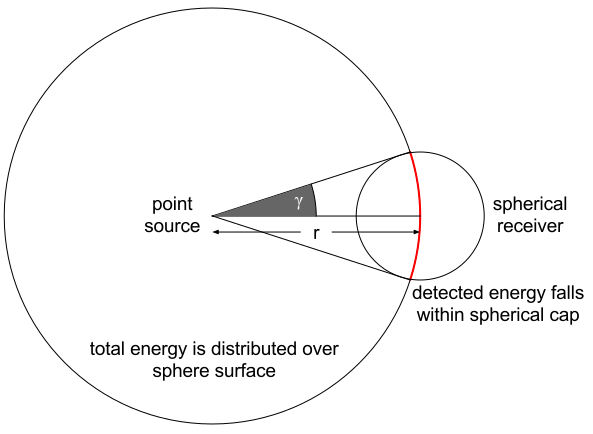
\includegraphics{images/detected_energy.pdf}
\caption{The proportion of uniformly-distributed rays intersecting the
receiver depends on the distance to the source, and opening angle formed
by the receiver. The acoustic intensity registered by the ray tracer is
given by the number of rays which intersect the receiver, and the energy
carried by each ray.\label{fig:detected_energy}}
\end{figure}

The direct energy in both models should be equal, so the two equations
can be set equal to one another, giving an equation for the initial
intensity of each ray, in terms of the source intensity
\(E_{\text{source}}\), the opening angle of the receiver \(\gamma\), and
the number of rays \(N\).

\begin{enumerate}
\def\labelenumi{(\arabic{enumi})}
\setcounter{enumi}{29}
\tightlist
\item
  \[
  \begin{aligned}
  E_{\text{ray tracer}} &= E_{\text{image source}} \\
  NE_r \left( \frac{1-\cos\gamma}{2} \right) &= \frac{E_{\text{source}}}{4\pi r^2} \\
  E_r &= \frac{E_{\text{source}}}{2 \pi r^2 N (1 - \cos\gamma)}
  \end{aligned}
  \]
\end{enumerate}

As long as the initial ray intensities are set according to this
equation, both methods will produce outputs with the correct relative
levels. The outputs from the two methods are combined by simple signal
addition, with no need for additional level adjustment.

\subsection{Geometric and Waveguide}\label{geometric-and-waveguide}

Setting the waveguide mesh level should follow a similar procedure. The
waveguide output level should be normalised so that the direct intensity
observed at the receiver is equal to that observed in the image-source
model. The normalisation is achieved through the use of a
\emph{calibration coefficient} which can be used to scale the waveguide
output, or alternatively to adjust the magnitude of the input signal.

Several suggestions for finding the calibration coefficient are
suggested in the literature. One option, which is perhaps the simplest
(short of manual calibration), is found in
{[}\protect\hyperlink{ref-southernux5fspatialux5f2011}{1}{]}. The
average magnitude of a certain frequency band is calculated for both the
waveguide and geometric output. The calibration coefficient is then
equal to the ratio of these two magnitudes. This approach is flawed, in
that the same frequency band must be used for both signals. This
frequency band will therefore be towards the lower end of the geometric
output, which is known to be inaccurate (this is the entire reason for
hybrid modelling), and at the to end of the waveguide output (which may
be inaccurate due to numerical dispersion). It is impossible to compute
an accurate calibration coefficient from inaccurate data.

Another method, suggested in the same paper
{[}\protect\hyperlink{ref-southernux5fspatialux5f2011}{1}{]}, is to find
the intensity produced by the waveguide at a distance of 1m, and then to
normalise both models so that they produce the same intensity at this
distance. The image-source direct response is low-pass filtered, so that
it only contains energy in the same frequency band as the waveguide
output. Then, the maximum magnitude in the initial portion (up to the
first reflection) of the output signal is found, for the image-source
and waveguide output. The calibration parameter is found by taking the
ratio of these maximum magnitudes. This differs from the first
technique, in that the calibration coefficient is derived from a single
contribution in the time-domain, instead of from frequency-domain
magnitudes accumulated over the entire duration of the signal.

The second method is superior, in that it will produce an accurate
calibration coefficient. Unfortunately, it requires analysis of the
waveguide output signal which, while not time-consuming, seems
unnecessary. A given mesh topology and excitation signal should always
require the same calibration coefficient, assuming that the geometric
source level remains constant. It should be possible to calculate the
calibration coefficient for a certain mesh topology, and then to re-use
this coefficient across simulations. This is the approach taken in
{[}\protect\hyperlink{ref-siltanenux5ffinite-differenceux5f2013}{60}{]}
which provides Wayverb's calibration method.

This general calibration coefficient is found by exciting a waveguide
mesh with an impulsive signal, and recording the pressure at a receiver
node immediately adjacent to the source node. The simulation continues
until the magnitude of vibrations at the receiver have reduced below
some threshold (perhaps falling below the noise floor). Now, the change
in pressure at a distance \(X\) is known, where \(X\) is the inter-nodal
spacing of the waveguide mesh. The geometric pressure level at the same
distance is given by

\begin{enumerate}
\def\labelenumi{(\arabic{enumi})}
\setcounter{enumi}{30}
\tightlist
\item
  \[ p_g=\sqrt{\frac{PZ_0}{4\pi}} / X \]
\end{enumerate}

where \(P\) is the source strength and \(Z_0\) is the acoustic impedance
of air. The waveguide pressure level cannot be directly compared to the
geometric pressure level, because the upper portion of the waveguide
output frequency range is invalid. Instead, the DC levels are compared.
The DC component of the waveguide output can be found simply by
accumulating the signal at the receiver. Now, the calibration
coefficient \(\eta\) can be expressed like so:

\begin{enumerate}
\def\labelenumi{(\arabic{enumi})}
\setcounter{enumi}{31}
\tightlist
\item
  \[\eta = \frac{p_\text{init}R}{p_\text{DC}X}\]
\end{enumerate}

where \(p_\text{init}\) and \(p_\text{DC}\) are the initial and DC
pressure levels respectively, \(X\) is the inter-nodal spacing, and
\(R\) is the distance at which the \emph{geometric} source has intensity
1W/m².

Experimentally-obtained values of \(\frac{p_\text{DC}}{p_\text{init}}\)
are given in
{[}\protect\hyperlink{ref-siltanenux5ffinite-differenceux5f2013}{60}{]}
for several different mesh topologies. To produce normalised waveguide
outputs, a calibration coefficient is calculated, using the experimental
result corresponding to a rectilinear mesh. The waveguide excitation is
then scaled by this calibration coefficient.

\subsubsection{Testing}\label{testing}

To validate the waveguide calibration procedure, a simple cuboid-shaped
room is simulated using the image-source and waveguide methods. The
outputs are compared in the frequency-domain, to ensure that the modal
responses of the two models match, in shape and in magnitude.

Although geometric methods are generally not capable of modelling
low-frequency modal behaviour, the image-source model in a geometric
room is a special case. For cuboid rooms with perfectly reflective
surfaces, the image-source method is exact
{[}\protect\hyperlink{ref-kuttruffux5froomux5f2009}{29}{]}, and it
remains reasonably accurate for slightly-absorbing surfaces. In cuboid
rooms the image-source model can, therefore, predict modal behaviour.
Additionally, for this room shape, the image source method can be
dramatically accelerated, making it possible to calculate extended
impulse responses
{[}\protect\hyperlink{ref-allenux5fimageux5f1979}{61}{]}. This
accelerated method differs from Wayverb's image-source finder, in that
it can calculate long impulse responses for one specific room shape,
whereas Wayverb's can calculate short responses for arbitrary geometry.

If the accelerated method is implemented, it can be used to generate
impulse responses which are close to ideal (depending on the surface
absorptions used). These impulse responses can be compared to those
produced by the waveguide, and if the calibration coefficient has been
chosen correctly, then their frequency responses should match.

A room, measuring \(5.56 \times 3.97 \times 2.81\) metres is simulated,
using the accelerated image-source and waveguide methods. The source is
placed at (1, 1, 1), with a receiver at (2, 3, 1.5). Both methods are
run at a sampling rate of 16KHz. The simulation is carried out three
times, with surface absorptions of 0.2, 0.1, and 0.05, and in all cases
the simulation is run up until the Sabine-estimated RT60, which is 0.52,
1.03 and 2.06 seconds respectively. The resulting frequency responses
are shown below\text{ (figure
\ref{fig:calibration})}.

\begin{figure}[htbp]
\centering
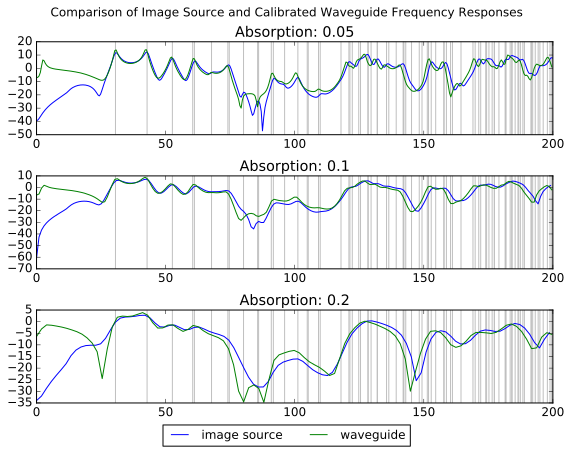
\includegraphics{images/calibration.pdf}
\caption{Frequency responses analysis of image-source and waveguide
outputs. The initial waveguide level has been calibrated using the
technique described above. Room mode frequencies are shown in
grey.\label{fig:calibration}}
\end{figure}

In the graphs, room modes are shown. One of the properties of the
waveguide is that it models wave effects which directly contribute to
this low-frequency modal behaviour. In the case of arbitrarily-shaped
rooms, the image model is not exact, and cannot be used to model
low-frequency behaviour in this way, while the waveguide will accurately
model low-frequency behaviour in any enclosed space. This is the main
reason for using a wave-modelling technique at all, instead of using
geometric methods for the entire spectrum.

Below 30Hz, the responses show significant differences. Between 30 and
70Hz, the responses match closely, to within a decibel. There is some
divergence at 80Hz, after which the results match closely again until
the upper limit of 200Hz. At the upper end of the spectrum, the levels
match closely between outputs, but the peaks and troughs are slightly
``shifted''.

The low-frequency differences can be explained as error introduced by
the hard-source/Dirac-delta waveguide excitation method (see
\href{\%7B\%7B\%20site.baseurl\%20\%7D\%7D\%7B\%\%20link\%20waveguide.md\%20\%\%7D}{Digital
Waveguide Mesh}). This source type has previously been demonstrated to
cause significant error at very low frequencies
{[}\protect\hyperlink{ref-sheafferux5fphysicalux5f2014}{54}{]}.

There are several possible causes for the remaining differences seen
between the outputs of the different models. Firstly, the image-source
technique is only exact for perfectly reflecting boundaries. The
boundary model used in this image-source implementation is the same
locally-reacting surface model that Wayverb uses: the reflection factor
is real-valued and angle-dependent. A more physically correct method
would be to use complex reflection factors, which would allow phase
changes at boundaries to be represented. The boundary model is almost
certainly the cause of the largest discrepancy, at around 80Hz: results
given in {[}\protect\hyperlink{ref-aretzux5fcombinedux5f2009}{4}, p.
78{]} show similar artefacts of the real-value angle-dependent
reflection factor, compared against other more accurate image-source
boundary types. Due to time constraints, these more complicated boundary
models could not be tested here.

The small frequency shift at the top of the spectrum is most likely to
be caused by numerical dispersion in the waveguide mesh. Numerical
dispersion becomes more pronounced as frequency increases, which is
consistent with the shift seen in the results, which is greater at
higher frequencies. The shift may also be caused by slight differences
in the dimensions of the modelled room, or the source and receiver
positions. In the image-source model, all measurements and positions are
exact, but the waveguide must ``quantise'' the boundary, source, and
receiver positions so that they coincide with mesh nodes. If the
dimensions of the room were adjusted slightly, this would also cause the
room modes to change (which again would be more pronounced at higher
frequencies), which might lead to a perceived spectral shift relative to
a room with exact dimensions.

Despite the small differences between the frequency responses, the close
level match between models suggests that the calibration coefficient is
correct.

The reverb times of the outputs are also compared and shown in the
following table.

\begin{table}[ht]
\centering

\caption{}

\begin{tabular}{@{}llll@{}}
\toprule

absorption & method & T20 / s & T30 / s \\\midrule

0.05 & exact image source & 1.044 & 1.065 \\
0.05 & waveguide & 1.165 & 1.180 \\
0.10 & exact image source & 0.5401 & 0.5633 \\
0.10 & waveguide & 0.5689 & 0.5905 \\
0.20 & exact image source & 0.2768 & 0.2990 \\
0.20 & waveguide & 0.2674 & 0.2880 \\

\bottomrule
\end{tabular}

\end{table}

There is a difference of 11\% for the lowest absorption, which falls to
6\% for an absorption of 0.10, and to 4\% for an absorption of 0.20.
Given that the image-source method is nearly exact in cuboid rooms,
these differences are small enough to suggest that the waveguide and its
boundary model have been implemented correctly.

\chapter{Microphone Modelling}\label{microphone-modelling}

\section{Introduction}\label{introduction-1}

In the preceding sections, simulation results have been recorded using a
virtual omnidirectional microphone model. This model records the sound
pressure at a single point in space. The gain and frequency response of
the receiver are not affected by the direction of the pressure gradient.
Signals recorded with omnidirectional microphones are primarily useful
for assessing the overall ``character'' of an acoustic space, including
reverb time, intelligibility, and overall gain.

However, one of the goals of room acoustics simulation is \emph{virtual
acoustics}: recreating the modelled auditory environment in such a way
that the listener believes they are hearing sounds within a physical
space. Real reverbs are highly directional, containing direct sound from
the source, and reflected sounds from the room boundaries. To produce a
convincing virtual environment, these directional cues must be encoded,
by adjusting the output gain and frequency response depending on the
direction of the cue. This is achieved using a direction-sensitive
receiver model.

\section{Background}\label{background-4}

Humans are able to detect the originating direction of sounds using two
main techniques: Interaural Time Difference (ITD) defines the time delay
between ears, when the sound source is located nearer to one ear than
the other; and Interaural Level Difference (ILD) denotes the difference
in sound level (which may vary by frequency) caused by attenuation by
the outer ear, head, and torso. The suitability of impulse responses for
stereo or multichannel playback depends on the ability to produce
signals with appropriate ITD and ILD, in such a way that each reflection
is perceived as coming from a certain direction.

When recording impulse responses of physical spaces, several techniques
might be used to retain ITD and ILD information.

One option is to record the impulse response using a matched pair of
microphones. An AB pair will capture interchannel time difference, but
will only capture interchannel level difference if the source is
positioned near to the microphones. Alternatively, an XY or Blumlein
pair will capture level difference, but will be incapable of recording
time difference because wave-fronts will always arrive at both capsules
simultaneously.

Microphone pair methods are only suitable for recording stereo signals,
as they only capture a two-dimensional ``slice'' through the modelled
scene, where all directional information is restricted to the same plane
as the microphone capsules. The technique can be extended to higher
dimensions by using more microphone capsules. This is the basis of the
ambisonic approach, which for B-format recordings uses four coincident
directional microphone capsules to capture the three-dimensional
directional pressure gradient and overall pressure level. Instead of
being used directly, the recorded signals are post-processed depending
on the configuration of the output speakers. For playback on headphones,
the signals can be filtered with \emph{head related transfer functions}
(HRTFs), which modify the frequency content of the sound depending on
its originating direction, mimicking the absorptive characteristics of
the human head and torso
{[}\protect\hyperlink{ref-noisternigux5f3dux5f2003}{62}{]}.

If it is known that the recording will only be reproduced on headphones,
the preferred method for capturing impulse responses which retain
appropriate ILD and ITD is to use in-ear microphones, or a ``dummy
head'' microphone pair. Recordings made in this way capture the ITD and
ILD that are caused by sonic interactions with the outer ear, head, and
torso, and produce a convincing reconstruction of the sonic space when
played back over headphones. However, responses recorded using this
technique are unsuitable for loudspeaker playback.

With the exception of the spaced-pair methods, all of these techniques
require that the receiver gain is dependent upon the incident direction.
The dummy head technique additionally requires that the frequency
response of the receiver is dependent upon the incident direction. To
allow reproduction on both headphones and arbitrary loudspeaker arrays,
the receiver model in Wayverb should encompass all of the techniques
described above. Given that spaced microphone techniques can be modelled
simply by including multiple receivers in the simulation, each virtual
capsule should have configurable direction-dependent gain and frequency
response, allowing it to behave like a standard microphone, or like the
ear of a dummy head.

\hypertarget{calculating-directional-gain}{\section{Calculating
Directional Gain}\label{calculating-directional-gain}}

Wayverb contains two different models for calculating an appropriate
gain from an incident direction, described here.

\subsection{Microphone}\label{microphone}

The first method, the ``perfect microphone'', is very simple. Given that
the virtual microphone is pointing in direction \(\hat{p}\), and has a
``shape'' parameter \(0 \leq s \leq 1\), the direction-dependent
attenuation \(a(\hat{d})\) from direction \(\hat{d}\) is given by

\begin{enumerate}
\def\labelenumi{(\arabic{enumi})}
\setcounter{enumi}{32}
\tightlist
\item
  \[a(\hat{d}) = (1 - s) + s(\hat{d} \cdot \hat{p})\]
\end{enumerate}

where \(\hat{p}\) and \(\hat{d}\) are unit vectors, and \(\cdot\) is the
dot-product operator. When \(s\) is set to 0, the \(a(\hat{d})\) is
equal to one for all values of \(\hat{d}\), modelling an omnidirectional
polar pattern. When \(s\) is 1, the modelled polar pattern is
bidirectional, with a gain of 1 in front the microphone, 0 at either
side, and -1 behind. When \(s\) is 0.5, the pattern is cardioid. Sub-
and supercardioid patterns are created by setting \(s\) lower or higher
than 0.5 respectively. This microphone model is flexible, allowing
almost all standard microphone techniques (including the XY pair,
Blumlein pair, and B-format ambisonic) to be simulated.

Note that this model has an ideally flat frequency response in every
direction, so it can only be used to model perfect microphones. It is
not suitable for modelling physical microphones with direction-dependent
frequency responses. In particular, with this technique it is not
possible to produce binaural dummy-head-style recordings, for immersive
headphone playback.

\subsection{HRTF}\label{hrtf}

A more general microphone model would allow specific per-frequency-band
gains to be set for each incoming direction. Such a model is implemented
in Wayverb, but is used only for the modelling of HRTF characteristics.
In the future, the approach could easily be extended to simulate general
non-flat microphones.

The method itself is based on a two-dimensional lookup table, indexed by
the azimuth and elevation angles formed by the incident direction. The
table is produced using experimentally-obtained HRTF data from the IRCAM
Listen database
{[}\protect\hyperlink{ref-oliverux5flistenux5f2003}{63}{]}. The data
takes the form of a collection of stereo audio files, containing the
impulse responses measured using microphones placed in the left and
right ears of a human volunteer. The recordings are made in an anechoic
environment. Each file contains the response measured for an impulse
originating at a specific azimuth and elevation.

To prepare the HRTF database for use in Wayverb, the audio files are
multi-band-filtered, using the same 8-band frequencies used throughout
Wayverb. Then, the per-band per-channel energy is recorded to a lookup
table.

To find the receiver frequency response for a given incident direction,
the direction vector is converted to an azimuth and an elevation. Then,
this azimuth and elevation are rounded to the closest angles which exist
in the lookup table. They are used to index the lookup table, and the
energies at that index are returned.

This model contains two approximations: the first is the directional
discretisation process, which ``quantises'' incoming angles to a set of
discrete, equally-spaced bins. In the final implementation,
fifteen-degree increments are used, matching the directional resolution
of the experimentally-obtained data. However, humans can localise sounds
from frontal sources to an accuracy of one degree
{[}\protect\hyperlink{ref-schroderux5fphysicallyux5f2011}{31}, p. 22{]},
so higher directional resolution may be required to produce a convincing
binaural effect. This resolution is of course limited by the directional
resolution of the input data, and HRTF data with one-degree resolution
would be time-consuming to measure, and expensive to store.

The second approximation is in the frequency resolution of the lookup
table. HRTF data is supplied as a set of finite-impulse-response filter
kernels, which represent continuous frequency spectra, up to the
sampling frequency of the kernels. Generally, these filter kernels would
be used via convolution, resulting in a precise adjustment of the
frequency content of the filtered signal. If this approach were to be
taken in Wayverb, it would require creating a separate output signal for
each of the incident directions, and then convolving each direction
separately, before a final mixdown. This would be extremely costly: for
separation angles of fifteen degrees, this means recording signals for
each of 288 incident directions, which might easily occupy more than a
gigabyte of memory (288 3-second impulse responses at 32-bits and
44.1KHz require 1160MB of memory), and then separately convolving and
mixing them. While this is definitely possible, it would be extremely
time consuming to run. By restricting the HRTF data to 8 frequency
bands, the application architecture can be simplified, while also
improving memory usage and runtime performance.

\section{Image Source Implementation}\label{image-source-implementation}

As described in the
\href{\%7B\%7B\%20site.baseurl\%20\%7D\%7D\%7B\%\%20link\%20image_source.md\%20\%\%7D}{Image
Source} section, the magnitude of the contribution of each image source
depends on the distance between the source and receiver, and the
direction-dependent reflectance characteristics of any intermediate
reflective surfaces. To model a directional receiver, the contribution
magnitude is additionally scaled by the receiver's gain in the direction
of that contribution.

The direction of each image source is found by subtracting the receiver
position from the image source position, and normalising the result.
This direction can either be used to directly compute the appropriate
attenuation factor, or it can be used to look up the attenuation in a
pre-computed table (see
\protect\hyperlink{calculating-directional-gain}{Calculating Directional
Gain} below).

In the case that the frequency response (rather than overall gain) of
the receiver depends on incident direction, a different attenuation
function or look-up table is used for each frequency band. At the end of
the simulation, the outputs in each band are band-pass filtered and
mixed down.

Wayverb includes a fast estimator for ITD in the image source model,
which has not been encountered in the literature. During the mix-down
process for the image-source contributions, the time of each
contribution is calculated based on the distance from the image source
to the receiver. When calculating these distances for the left ear, the
receiver position can be temporarily moved 10cm to the left, relative to
the receiver orientation, and the same can be done for the right ear.
The output signal will then incorporate small time delays between
channels, depending on the distance and direction of each image source.
This method relies on the assumption that all image sources are visible
from both ear positions, and that the new ear positions do not affect
the angle-dependent reflection characteristics of intermediate surfaces.
This is a reasonable assumption, given that the distance between ears is
generally small compared to the size of the modelled room. The benefit
of this method is that the costly image-source-finding process only has
to be run once in total, instead of once for each ear.

This image-source ``offsetting'' technique cannot be applied to
Wayverb's other simulation methods. In the waveguide, the new ``ear''
positions may not fall directly on grid nodes, and so the waveguide
simulation would have to be run twice, with different grids. The
raytracer would not benefit from interaural time difference at all, as
the maximum possible interaural time delay is the interaural distance
divided by the speed of sound, 0.2/340=0.0005s, which is less than the
1ms energy histogram sampling interval. Therefore, any measured ITD
would be lost when quantising to the histogram interval.

The drawback of the offsetting method is that, if the user manually
positions two receivers with appropriate interaural spacing, an extra
offset will still be automatically applied. This will lead to an
interaural spacing that is twice as wide as desired. This could be
addressed by including an option in the software to enable or disable
the additional offset. Due to time constraints this feature has not been
implemented in the current version of Wayverb.

\section{Ray Tracer Implementation}\label{ray-tracer-implementation}

In the ray tracer, a very similar approach could be taken. The incident
direction of each ray is known, so this direction might be used with a
function or lookup-table to adjust the ray's multiband intensity before
it is added to the energy histogram (see
\href{\%7B\%7B\%20site.baseurl\%20\%7D\%7D\%7B\%\%20link\%20ray_tracer.md\%20\%\%7D}{Ray
Tracer}).

In terms of implementation, this approach would be needlessly expensive.
In Wayverb, the initial simulation and directional processing stages are
kept separate, allowing a single simulation to be processed by several
different virtual microphone capsules. While flexible, it is also
infeasible to store the direction of each incident ray, especially if
there are hundreds of thousands of rays in the simulation. The ray
tracer is used to estimate the late reverberation of the space, in which
individual sonic events are ``blurred'' together, and in which there are
few directional cues
{[}\protect\hyperlink{ref-schroderux5fphysicallyux5f2011}{31}, p. 21{]},
so this level of per-ray directional accuracy is unnecessary.

Instead, the surface of the spherical receiver is divided into discrete
\emph{directivity groups}, mirroring the approach of Schroder in
{[}\protect\hyperlink{ref-schroderux5fphysicallyux5f2011}{31}, p. 72{]}.
A separate multiband energy histogram is maintained for each directivity
group, where the direction of ray incidence determines the histogram
used to store that ray's energy. These histograms are at a substantially
lower sampling-frequency than the output sampling rate, so it is
feasible to store one for each discrete incident direction, as long as
the direction quantisation intervals are on the order of ten to twenty
degrees. To generate audio-rate results, the directional histograms must
be combined into a single energy histogram, which can then be used to
weight a noise sequence as discussed in the
\href{\%7B\%7B\%20site.baseurl\%20\%7D\%7D\%7B\%\%20link\%20ray_tracer.md\%20\%\%7D\%7D}{Ray
Tracer} section. This achieved by taking the centre direction of each
directivity group, calculating or looking-up the correct attenuation for
that direction, and then multiplying the entire histogram by that value.
The final direction-weighted histogram is given by the elementwise sum
of all individual weighted histograms.

\section{DWM Implementation}\label{dwm-implementation}

\subsection{Implementation Decisions}\label{implementation-decisions}

Implementing directional receivers in the waveguide mesh is more
complicated than for the geometric methods. Although absolute pressure
values are available in the mesh, directional pressure values are not
inherently supported. In order to simulate a directional receiver, the
instantaneous direction of the sound field must be found at the receiver
point. Several methods were considered, as outlined below.

\subsubsection{Blumlein Difference
Technique}\label{blumlein-difference-technique}

The first method, described in
{[}\protect\hyperlink{ref-southernux5fmethodsux5f2007}{64}{]} and
{[}\protect\hyperlink{ref-southernux5f2ndux5f2007}{65}{]}, is designed
with the goal of encoding the 3D sound-field by means of spherical
harmonic decomposition to the second order, for use in ambisonic
reproduction.

This method is based on sound intensity probe theory, which allows
directional velocity components of a sound field to be captured using
two closely-spaced omnidirectional receivers. In the DWM, each node has
an associated pressure, so two closely-spaced nodes can be used to
emulate a pair of omnidirectional receivers, and in turn used to
generate directional velocity components. A full first-order B-format
signal can be made using seven such ``pressure sensors'', arranged in a
cross shape, with a single node at the centre, and six nodes placed
around it. The pressure field velocity components are found by
subtracting nodes on ``opposite'' sides of the cross, while the centre
node contributes the overall pressure at the receiver. A second-order
output is achieved by adding further pressure-sensing nodes in between
the first-order nodes.

Note that this technique does not allow the immediate production of
directional responses. Instead, it is designed to produce outputs in
ambisonic format, which are then post-processed to create a signal with
the desired modelled directional response.

Additionally, this technique has some difficulty adapting to meshes with
large grid spacings. In a rectilinear mesh, the seven first-order nodes
can be placed exactly, as their positions will coincide with nodes in
the mesh. However, the second-order nodes will not fall exactly on
existing nodes, and instead their positions will need to be quantised to
the closest mesh nodes. This problem becomes worse in other mesh
topologies, such as the tetrahedral mesh, where it may be that very few
of the sensor nodes can be exactly placed in the desired positions.

To facilitate more exact placement of sensor nodes, the spatial sampling
frequency of the mesh must be increased (by reducing the grid spacing,
the quantisation error in the sensor placement is also reduced). The
example given in
{[}\protect\hyperlink{ref-southernux5f2ndux5f2007}{65}{]} uses a sensor
spacing of 0.04 metres, giving a maximum valid sampling frequency of
4.25kHz. However, to allow accurate placement of these sensors, a grid
with a spacing of 0.0027m is required. This increase in mesh density
necessitates more than 3000 times the original number of nodes, which is
only practical for very small modelled spaces.

Finally, this method places an additional constraint on the portion of
the spectrum of the output signal which may be considered valid. The
maximum valid frequency of the output spectrum is determined by the
ratio between the receiver spacing and the wavelength at that frequency.
To raise the upper frequency limit, the receiver spacings must be made
as small as possible, which requires costly mesh oversampling. Small
receiver spacings reduce the sensitivity at the lower end of the
spectrum, so ideally the simulation will use several sets of receiver
nodes with different spacings, in order to maintain a flat frequency
response.

This technique seems suitable for calculating lower-order ambisonic
signals in small modelled spaces. For higher order outputs, with
consistent frequency responses across the spectrum, the technique
quickly becomes too expensive (due to mesh oversampling) and complex to
implement (as several receiver spacings and configurations are required
for a single simulation output).

\subsubsection{Intensity Calculation
Technique}\label{intensity-calculation-technique}

The second method considered for implementation in Wayverb is described
by Hacıhabiboglu in
{[}\protect\hyperlink{ref-hacihabibogluux5fsimulationux5f2010}{66}{]}.
This method is based around estimating the acoustic intensity at the
output node of the DWM.

The technique is much more straight-forward than the technique discussed
above. The pressure differences between the ``output'' node and its
surrounding nodes are calculated. These pressures are transformed
depending on the relative positions of each surrounding node, and
combined to produce a three-element vector containing an approximation
for the three-dimensional pressure gradient. The equations describing
these operations in the general case are not replicated here, however
they may be greatly simplified in the rectilinear case, as will be shown
in the \protect\hyperlink{implementation-3}{Implementation} section
below. The velocity for each time step is found by adding the pressure
gradient vector to the velocity at the previous time step, where the
initial velocity is assumed to be zero. Intensity is found by
multiplying this velocity by the pressure at the output node.

In some respects, this technique is very similar to the Blumlein
difference technique. Both techniques calculate the instantaneous
pressure gradient at the output node by subtracting the pressures of the
surrounding nodes. The main difference is that the Blumlein method
requires that the mesh pressure is found at exact locations relative to
the output node, which often requires mesh oversampling. The intensity
calculation technique instead uses a more general matrix-based method,
which incorporates the relative node positions into the calculation. In
short, the Blumlein method requires that the mesh is designed to suit
the receiver configuration, whereas the intensity calculation method can
adapt to arbitrary mesh topologies and spacings.

The frequency range issues mentioned in
{[}\protect\hyperlink{ref-southernux5fmethodsux5f2007}{64}{]} (where
large mesh spacings reduce the output bandwidth, and low mesh spacings
reduce low frequency sensitivity) are mentioned by Hacıhabiboglu in
{[}\protect\hyperlink{ref-hacihabibogluux5fsimulationux5f2010}{66}{]}.
It is unclear whether the intensity calculation technique solves this
problem, although the results presented in
{[}\protect\hyperlink{ref-hacihabibogluux5fsimulationux5f2010}{66}{]}
appear consistent across the spectrum. Some inaccuracy is evident at the
top of the spectrum, but this is attributed to direction-dependent
dispersion error, rather than to a problem with the frequency response
of the model itself.

Under this scheme, the output of the waveguide mesh is actually two
streams of information: a stream of scalar values describing the
pressure at the output node; and a stream of 3D vectors denoting the
directional intensity at that point.

To find the directional response for a single time-step, the intensity
vector is used to look up the microphone response in the direction of
the vector, which is a scalar value. The microphone response is squared,
and multiplied by the magnitude of the intensity vector, yielding a
positive scalar output. Finally, the sign of the actual pressure at the
output node is copied to the output value. To find the full directional
response, this process is repeated for every time-step of the
simulation.

The intensity calculation technique can also model receivers with
direction-dependent frequency responses. The intensity and pressure
outputs are processed with a set of polar patterns corresponding to
responses at different frequency bands. Then, these processed signals
are band-passed with linear-phase filters, and summed together.

\subsubsection{Choice of Method}\label{choice-of-method}

The intensity calculation technique was chosen for implementation in
Wayverb, as it is simpler to implement, and less expensive to run. Also,
the Blumlein difference technique is only practical in rectilinear
meshes, whereas the intensity calculation technique can be adapted to
any mesh topology. This was an important consideration at the beginning
of the Wayverb project, which originally used the tetrahedral mesh due
to its relative efficiency.

\hypertarget{implementation-3}{\subsection{Implementation}\label{implementation-3}}

The implementation is very simple in the rectilinear mesh. The mesh is
inherently aligned to the axial directions, which means that the matrix
maths is greatly simplified. The process for finding the instantaneous
intensity vector for each step of the waveguide simulation is shown in
pseudocode below.

\begin{Shaded}
\begin{Highlighting}[]
\KeywordTok{def} \NormalTok{compute_intensities_at_node(node_position,}
                                \NormalTok{mesh_spacing,}
                                \NormalTok{mesh_sample_rate,}
                                \NormalTok{ambient_density):}
    \NormalTok{velocity_vector }\OperatorTok{=} \NormalTok{(}\DecValTok{0}\NormalTok{, }\DecValTok{0}\NormalTok{, }\DecValTok{0}\NormalTok{)}
    \NormalTok{pressures }\OperatorTok{=} \NormalTok{[]}
    \NormalTok{intensities }\OperatorTok{=} \NormalTok{[]}

    \NormalTok{(nx_position, px_position,}
     \NormalTok{ny_position, py_position,}
     \NormalTok{nz_position, pz_position) }\OperatorTok{=} \NormalTok{compute_neighbouring_positions(node_position)}

    \ControlFlowTok{for} \NormalTok{step }\OperatorTok{in} \NormalTok{waveguide:}
        \OperatorTok{//}  \NormalTok{Find current pressure at output node.}
        \NormalTok{p }\OperatorTok{=} \NormalTok{get_node_pressure(node_position)}

        \OperatorTok{//}  \NormalTok{Calculate the pressure differences between surrounding nodes.}
        \NormalTok{nx_difference }\OperatorTok{=} \NormalTok{(get_node_pressure(nx_position) }\OperatorTok{-} \NormalTok{p) }\OperatorTok{/} \NormalTok{mesh_spacing}
        \NormalTok{px_difference }\OperatorTok{=} \NormalTok{(get_node_pressure(px_position) }\OperatorTok{-} \NormalTok{p) }\OperatorTok{/} \NormalTok{mesh_spacing}
        \NormalTok{ny_difference }\OperatorTok{=} \NormalTok{(get_node_pressure(ny_position) }\OperatorTok{-} \NormalTok{p) }\OperatorTok{/} \NormalTok{mesh_spacing}
        \NormalTok{py_difference }\OperatorTok{=} \NormalTok{(get_node_pressure(py_position) }\OperatorTok{-} \NormalTok{p) }\OperatorTok{/} \NormalTok{mesh_spacing}
        \NormalTok{nz_difference }\OperatorTok{=} \NormalTok{(get_node_pressure(nz_position) }\OperatorTok{-} \NormalTok{p) }\OperatorTok{/} \NormalTok{mesh_spacing}
        \NormalTok{pz_difference }\OperatorTok{=} \NormalTok{(get_node_pressure(pz_position) }\OperatorTok{-} \NormalTok{p) }\OperatorTok{/} \NormalTok{mesh_spacing}

        \OperatorTok{//}  \NormalTok{Find the instantaneous pressure gradient.}
        \NormalTok{pressure_gradient_vector }\OperatorTok{=} \NormalTok{((px_difference }\OperatorTok{-} \NormalTok{nx_difference) }\OperatorTok{/} \DecValTok{2}\NormalTok{,}
                                    \NormalTok{(py_difference }\OperatorTok{-} \NormalTok{ny_difference) }\OperatorTok{/} \DecValTok{2}\NormalTok{,}
                                    \NormalTok{(pz_difference }\OperatorTok{-} \NormalTok{nz_difference) }\OperatorTok{/} \DecValTok{2}\NormalTok{)}

        \OperatorTok{//}  \NormalTok{Update the velocity accumulator.}
        \NormalTok{velocity_vector }\OperatorTok{-=} \NormalTok{(pressure_gradient_vector }\OperatorTok{/}
                            \NormalTok{(ambient_density }\OperatorTok{*} \NormalTok{mesh_sample_rate))}

        \OperatorTok{//}  \NormalTok{Find the instantaneous intensity.}
        \NormalTok{intensity_vector }\OperatorTok{=} \NormalTok{velocity_vector }\OperatorTok{*} \NormalTok{p}

        \NormalTok{pressures.append(p)}
        \NormalTok{intensities.append(intensity_vector)}

    \ControlFlowTok{return} \NormalTok{pressures, intensities}
\end{Highlighting}
\end{Shaded}

For each waveguide step, the pressure and intensity at the output node
is found and stored. If there are multiple coincident capsules, then the
same pressure-intensity data can be post-processed once for each virtual
capsule, without needing to re-run the simulation. However, this
approach may not be well-justified: according to Hacihabiboglu et al.
this microphone model is only suitable for single-diaphragm directional
microphones, and is unsuitable for coincident pressure gradient
microphones with multiple elements
{[}\protect\hyperlink{ref-hacihabibogluux5fsimulationux5f2010}{66}{]}.
Despite its unsuitability, there is no other possible way of modelling
coincident capsules using this microphone model, so coincident capsules
\emph{are} allowed in Wayverb. Development of a microphone model with
better support of coincident capsules is a topic for future research.

Having generated the pressures and the intensity vectors at the output
node, the post-processing progresses by finding the magnitude of the
intensity vector. This value is multiplied by the square of the
polar-pattern attenuation in the direction of the intensity vector, and
then the square root is taken. Finally, the sign of the pressure is
copied to this output value. This process is repeated for each step of
the simulation, resulting in a sequence of directionally-processed
pressure values.

For binaural results, this process is repeated once for each frequency
band, resulting in several differently-weighted broadband signals. The
directional gains are found using the same lookup-table technique as the
geometric methods, using the azimuth and elevation of the intensity
vector as indices. The final output is created by bandpass filtering
each of these broadband signals using a zero-phase frequency-domain
filter, and then mixing them down. The filtering process is the same as
that used throughout Wayverb (see
\href{\%7B\%7B\%20site.baseurl\%20\%7D\%7D\%7B\%\%20link\%20ray_tracer.md\%20\%\%7D}{Ray
Tracer}).

\subsection{Testing of the Microphone Model in the
DWM}\label{testing-of-the-microphone-model-in-the-dwm}

The testing procedure is similar to that described in
{[}\protect\hyperlink{ref-hacihabibogluux5fsimulationux5f2010}{66}{]}. A
receiver is placed at the centre of a room measuring
\(1.5 \times 1.5 \times 1.5\) metres. Sixteen equally-spaced source
positions are generated in a circle with radius 1m around the receiver.
For each source, the room is simulated using a rectilinear waveguide
mesh with a sampling rate of 50KHz, for 294 steps. The step number is
chosen so that the initial wave-front will reach the receiver, but
reflections from the room walls will not. After each simulation, the
directionally-weighted signal recorded at the receiver is split into
frequency bands, and the normalised energy per band is calculated. The
bands are split in the frequency domain, using the frequency-domain
envelope method mentioned in the
\href{\%7B\%7B\%20site.baseurl\%20\%7D\%7D\%7B\%\%20link\%20ray_tracer.md\%20\%\%7D}{Ray
Tracer} section. The normalised energy of the band is calculated by
dividing the sum of squared bin magnitudes in the output by the
integrated frequency-domain envelope.

The per-band normalised energy can now be plotted against the angle of
incidence, and compared to the ideal polar pattern of the modelled
microphone. This is achieved by normalising the measured directional
response relative to the response in the front direction. If there is a
close match, then the model is successful.

Three different microphone polar patterns are simulated:
omnidirectional, bidirectional, and cardioid. The results are shown in
the following
figures\text{ (\ref{fig:omnidirectional} to \ref{fig:bidirectional})}.

\begin{figure}[htbp]
\centering
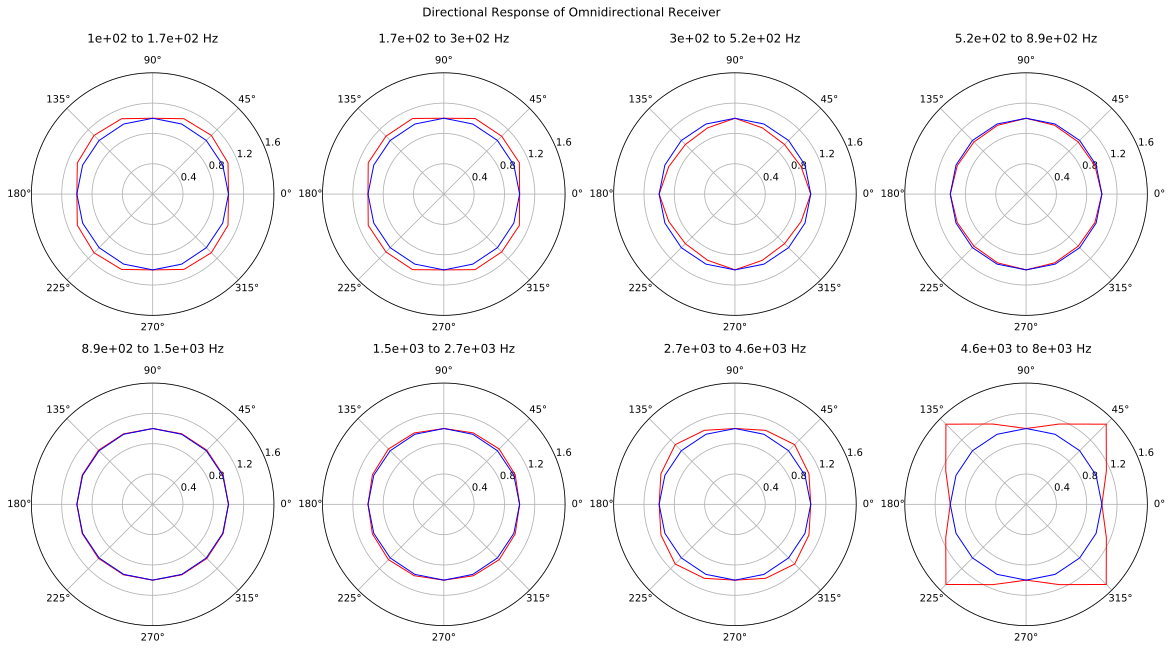
\includegraphics{images/Omnidirectional_response.pdf}
\caption{The directional response of an omnidirectional receiver in the
waveguide mesh.\label{fig:omnidirectional}}
\end{figure}

\begin{figure}[htbp]
\centering
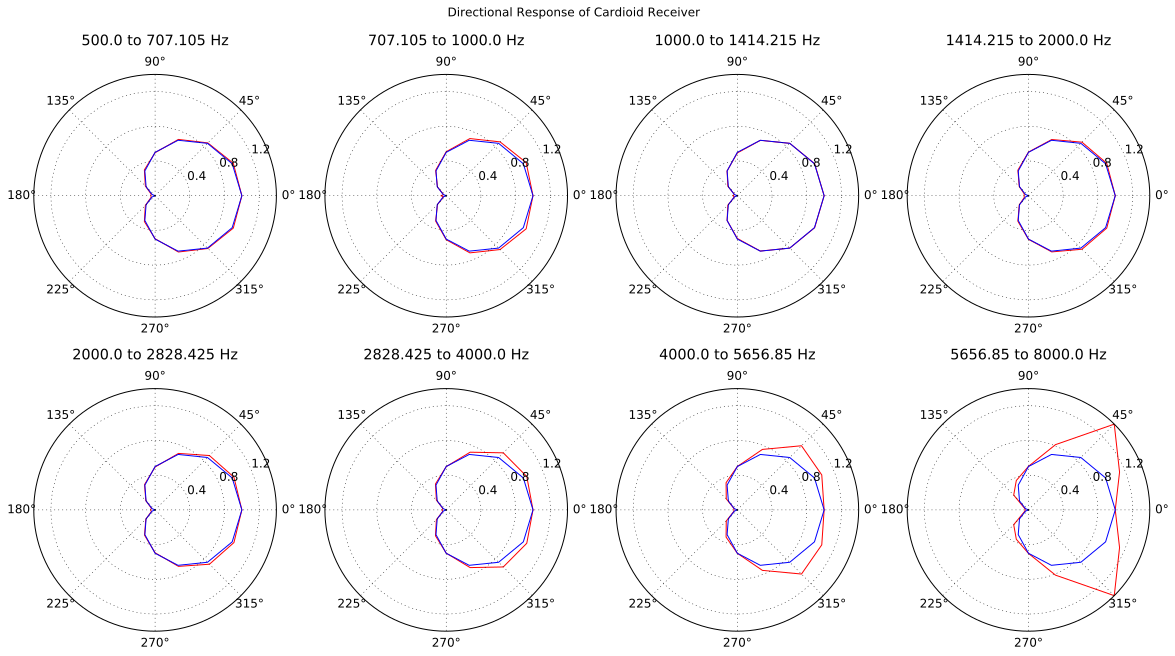
\includegraphics{images/Cardioid_response.pdf}
\caption{The directional response of a cardioid receiver in the
waveguide mesh.\label{fig:cardioid}}
\end{figure}

\begin{figure}[htbp]
\centering
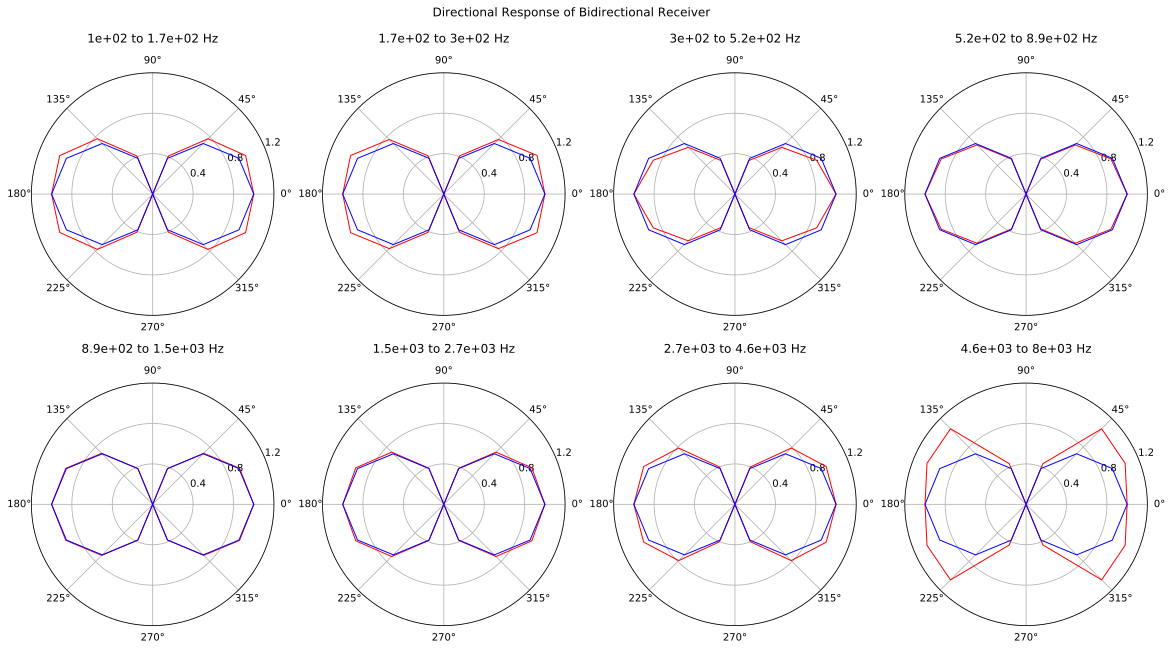
\includegraphics{images/Bidirectional_response.pdf}
\caption{The directional response of a bidirectional receiver in the
waveguide mesh.\label{fig:bidirectional}}
\end{figure}

Results are consistent across all polar patterns tested. At low
frequencies, the match is particularly good, with virtually no error in
all directions. As frequency increases, the error increases greatly.
This happens as a result of frequency-dependent dispersion. At higher
frequencies, the speed of wave-fronts changes depending on their
direction. In the rectilinear mesh, there is no dispersion along
diagonal directions
{[}\protect\hyperlink{ref-kowalczykux5froomux5f2011}{35}{]}. Along axial
directions, however, high-frequency wave-fronts move more slowly. This
is likely the cause of the predominant ``spikes'' seen in the diagonal
directions: in these directions, all the acoustic energy reaches the
receiver, while along axial directions, the wave-fronts are slower, and
the full energy does not reach the receiver within the simulation
window.

These results mirror those seen by Hacıhabiboglu, who also records
similar large errors in diagonal directions in the highest (8KHz) band.
These errors are also attributed to directional dispersion. Therefore,
error in the results is likely due to the properties of the waveguide
and the particular receiver technique used, rather than an error in the
implementation.

Although there is very large error in some directions at high
frequencies, at low frequencies this method produces accurate
directional responses. Even at higher frequencies (relative to the mesh
sampling rate), the response follows the same overall shape as the
desired response, so even here the results may provide a reasonable
approximation of the directional room response. Finally, if accurate
directional responses are required at higher frequencies, the mesh can
be oversampled to reduce directional dispersion. Although costly, it is
at least potentially possible to produce very accurate responses using
this method.

\chapter{Boundary Modelling}\label{boundary-modelling}

\section{Introduction}\label{introduction-2}

The ideal boundary model would allow complete control over the
frequency- and direction-dependent absorption and scattering of a
surface. Though this is reasonably straightforward to implement in
geometric models, it is far from a solved problem for the digital
waveguide mesh (DWM). Several possible implementations are discussed in
the literature, each with unique drawbacks.

This section will begin by discussing the ideal behaviour of modelled
acoustic boundaries. Then, the implementation for geometric models will
be discussed. Possibilities for DWM boundary models will be
investigated, and the final choice of method explained. The geometric
and DWM implementations will be evaluated and compared, to ensure
equivalence.

\section{Background}\label{background-5}

The books by Vorlander
{[}\protect\hyperlink{ref-vorlanderux5fauralization:ux5f2007}{30}, p.
35{]} and Kuttruff
{[}\protect\hyperlink{ref-kuttruffux5froomux5f2009}{29}, p. 35{]} both
devote entire chapters to the topic of sound reflection and scattering.
Please refer to these books for a detailed and broad explanation of
reflection effects. To avoid unnecessary duplication, this background
will be brief, aiming only to put terminology and decisions in context.

\subsection{Magnitude and Phase}\label{magnitude-and-phase}

The reflection factor \(R\) is a complex value given by

\begin{enumerate}
\def\labelenumi{(\arabic{enumi})}
\setcounter{enumi}{33}
\tightlist
\item
  \[R=|R|\exp(i\chi)\]
\end{enumerate}

which describes a modification to the amplitude and phase of a wave
reflected in a boundary (\(|R|\) is the magnitude term, \(\chi\) is
phase).

This factor depends both on the frequency and direction of the incident
wave. When \(\chi = \pi\)\$, \(R\) is negative, corresponding to a phase
reversal. This is known as a ``soft'' wall, but is rarely seen in room
acoustics. It is reasonable to assume that reflections are in-phase in
the majority of architectural acoustics problems
{[}\protect\hyperlink{ref-kuttruffux5froomux5f2009}{29}, p. 36{]}.

The wall impedance \(Z\) is defined as the ratio of sound pressure to
the normal component of particle velocity at the wall surface. It is
related to the reflection factor by

\begin{enumerate}
\def\labelenumi{(\arabic{enumi})}
\setcounter{enumi}{34}
\tightlist
\item
  \[R=\frac{Z\cos\theta-Z_0}{Z\cos\theta+Z_0}\]
\end{enumerate}

where \(\theta\) is the angle of incidence, and \(Z_0\) is the
characteristic impedance of the propagation medium, normally air. In the
case that the wall impedance is independent of the wave
angle-of-incidence, the surface is known as \emph{locally reacting}. A
locally reacting surface does not transmit waves tangentially along the
wall surface. In Wayverb, all surfaces are modelled as locally reacting.

The absorption coefficient \(\alpha\) of a wall describes the proportion
of incident energy which is lost during reflection. It is defined as

\begin{enumerate}
\def\labelenumi{(\arabic{enumi})}
\setcounter{enumi}{35}
\tightlist
\item
  \[\alpha =1-|R|^2\]
\end{enumerate}

\subsection{Scattering}\label{scattering}

The reflection factor, absorption coefficient, and wall impedance
describe the behaviour of perfectly-reflected (specular) waves. If the
reflecting surface has imperfections or details of the same order as the
wavelength, as many surfaces in the real world do, then some components
of the reflected wave will be \emph{scattered} instead of specularly
reflected.

Describing the nature of the scattered sound is more complicated than
specular reflections. A common method is to use a \emph{scattering
coefficient}, which describes the proportion of outgoing energy which is
scattered, and which may be dependent on frequency
\text{(see figure \ref{fig:scattering})}. The total outgoing energy
\(E_\text{total}\) is related to the incoming energy
\(E_\text{incident}\) by

\begin{enumerate}
\def\labelenumi{(\arabic{enumi})}
\setcounter{enumi}{36}
\tightlist
\item
  \[E_{\text{total}}=E_{\text{incident}}(1-\alpha)\]
\end{enumerate}

Then the scattering coefficient \(s\) defines the proportion of this
outgoing energy which is reflected specularly \(E_\text{specular}\) or
scattered \(E_\text{scattered}\):

\begin{enumerate}
\def\labelenumi{(\arabic{enumi})}
\setcounter{enumi}{37}
\tightlist
\item
  \[
  \begin{aligned}
  E_{\text{specular}} & =E_{\text{incident}}(1-\alpha)(1-s) \\
  E_{\text{scattered}} & =E_{\text{incident}}(1-\alpha)s
  \end{aligned}
  \]
\end{enumerate}

\begin{figure}[htbp]
\centering
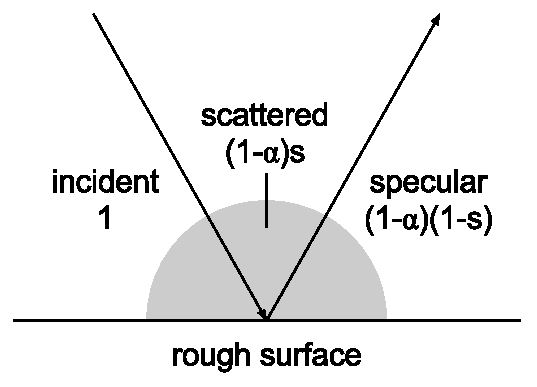
\includegraphics{images/scattering.pdf}
\caption{Reflected components from a rough
surface.\label{fig:scattering}}
\end{figure}

Alone, the scattering coefficient fails to describe the directional
distribution of scattered energy. In the case of an ideally-diffusing
surface, the scattered energy is distributed according to Lambert's
cosine law. That is, the intensity depends only on the cosine of the
outgoing scattering angle, and is independent of the angle of incidence
\text{(see figure
\ref{fig:lambert})}. More complex scattering distributions, which also
depend on the outgoing direction, are possible
{[}\protect\hyperlink{ref-christensenux5fnewux5f2005}{40}{]},
{[}\protect\hyperlink{ref-duranyux5fanalyticalux5f2015}{67}{]}, but
there is no single definitive model to describe physically-accurate
scattering.

\begin{figure}[htbp]
\centering
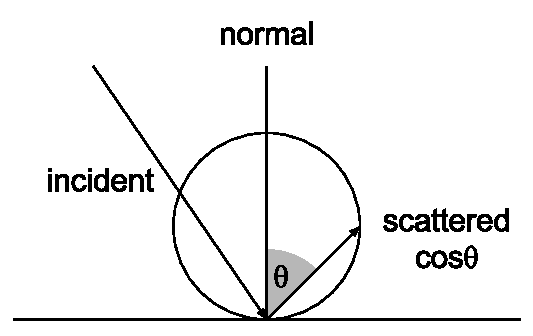
\includegraphics{images/lambert.pdf}
\caption{Lambert scattering. Scattered intensity is independent of
incident angle.\label{fig:lambert}}
\end{figure}

\section{Geometric Implementation}\label{geometric-implementation}

In both image-source and ray tracing methods, each ray starts with a
certain intensity or pressure. During a specular reflection, the ray
pressure must be multiplied by the wall reflection coefficient, to find
the outgoing pressure. All surfaces in Wayverb are locally reacting, so
the reflectance coefficient of a locally reacting surface must be
defined.

The \emph{specific acoustic impedance} \(\xi\) for a given surface is
defined as the impedance of that surface \(Z\) divided by the acoustic
impedance of the propagation medium (air) \(Z_0\).

\begin{enumerate}
\def\labelenumi{(\arabic{enumi})}
\setcounter{enumi}{38}
\tightlist
\item
  \[\xi=\frac{Z}{Z_0}\]
\end{enumerate}

Inserting this equation into (35) gives:

\begin{enumerate}
\def\labelenumi{(\arabic{enumi})}
\setcounter{enumi}{39}
\tightlist
\item
  \[R=\frac{\xi\cos\theta-1}{\xi\cos\theta+1}\]
\end{enumerate}

where \(\theta\) is the angle of incidence
{[}\protect\hyperlink{ref-southernux5froomux5f2013}{26}{]}.

For a general surface, \(\xi\) will be a function of the incident angle.
However, in the case of a locally reacting surface, the impedance is
independent of the angle of incidence. The \(\xi\) term in (40) can then
be replaced by \(\xi_0\) which represents the normal-incidence specific
impedance (which will be constant for all angles). Thus, the reflection
factor of a locally reacting surface is

\begin{enumerate}
\def\labelenumi{(\arabic{enumi})}
\setcounter{enumi}{40}
\tightlist
\item
  \[R=\frac{\xi_0\cos\theta-1}{\xi_0\cos\theta+1}\]
\end{enumerate}

Surfaces in Wayverb are defined in terms of absorption coefficients. To
express the reflectance in terms of absorption, an equation for
\(\xi_0\) in terms of absorption must be found, and substituted into
(41).

Assuming that the absorption coefficients denote normal-incidence
absorption, then by rearranging (36), the normal-incidence reflection
coefficient \(R_0\) is given by

\begin{enumerate}
\def\labelenumi{(\arabic{enumi})}
\setcounter{enumi}{41}
\tightlist
\item
  \[R_0=\sqrt{1-\alpha}\]
\end{enumerate}

\(R_0\) can also be expressed by setting \(\theta\) to 0 in (41):

\begin{enumerate}
\def\labelenumi{(\arabic{enumi})}
\setcounter{enumi}{42}
\tightlist
\item
  \[R_0=\frac{\xi_0 -1}{\xi_0 +1}\]
\end{enumerate}

To express \(\xi_0\) in terms of \(\alpha\), (43) is rearranged in terms
of the normal-incidence reflection coefficient:

\begin{enumerate}
\def\labelenumi{(\arabic{enumi})}
\setcounter{enumi}{43}
\tightlist
\item
  \[\xi_0=\frac{1+R_0}{1-R_0}\]
\end{enumerate}

Then, (42) may be substituted into (44) to give \(\xi_0\) in terms of
\(\alpha\). This new definition of \(\xi_0\) can then be used in
conjunction with (41) to define the angle-dependent reflection factor of
a locally reacting surface.

In Wayverb, surfaces may have different absorptions in each frequency
band. Each ray starts with the same pressure in each band. During a
specular reflection, the per-band absorptions are converted into
per-band reflection factors. Then, the pressure in each band is adjusted
using that band's reflection coefficient. This is similar to the
approach taken in graphical ray tracing, in which each ray carries
separate red, green, and blue components. These components are modified
independently, depending on the colour of the reflective surface.

By definition, image-source models find only specular reflections
(i.e.~image sources), so scattering is not implemented in these models.
Scattering can be implemented in ray tracers, but there is no consensus
on the optimum method. One option is to spawn two rays at every
reflection: a specular ray, and a diffuse ray with random direction.
Though this properly replicates the theory, it leads to an explosion in
the number of rays which must be traced, so is impractical in most
cases. A second option is to decide, using the scattering coefficient as
a probability, whether the reflection should be specular or diffuse
{[}\protect\hyperlink{ref-saviojaux5foverviewux5f2015}{2}{]}. This
solves the ray-explosion problem, but requires an additional random
number to be generated per-reflection, which can be costly for large
numbers of rays. An elegant solution is to simply mix the specular and
diffuse rays together, using the scattering coefficient as a weighting
{[}\protect\hyperlink{ref-rindelux5fuseux5f2000}{68}{]}, a technique
known as \emph{vector based scattering}
{[}\protect\hyperlink{ref-christensenux5fnewux5f2005}{40}{]}. This is
the approach taken by Wayverb. A major drawback of all these scattering
methods is that the scattering coefficient can only be
frequency-dependent if a separate ray is traced for each band. If a
single ray is used to carry all frequency components, then each
component must be scattered in exactly the same way.

The plain scattering model affects only the ongoing ray direction and
amplitude. However, it is worth considering that, at each reflection,
the scattered energy may be directly visible to the receiver. This fact
is exploited by the \emph{diffuse rain} technique
{[}\protect\hyperlink{ref-schroderux5fphysicallyux5f2011}{31}, pp.
61--66{]}, in which each reflection is considered to spawn a ``secondary
source'' which emits scattered energy towards the receiver. This
scattered energy is recorded only if the secondary source is visible
from the receiver.

The magnitude of scattered energy is proportional to the scattering
coefficient, and the Lambert diffusion coefficient. It is also
proportional to the fraction of the available hemispherical output area
which is covered by the receiver volume. The absolute area covered by a
spherical receiver \(A_{\text{intersection}}\) is found using the
equation for the surface area of a spherical cap.

\begin{enumerate}
\def\labelenumi{(\arabic{enumi})}
\setcounter{enumi}{44}
\tightlist
\item
  \[A_{\text{intersection}} = 2\pi r^2(1-\cos\gamma)\]
\end{enumerate}

Then, the detected scattered energy can be derived
{[}\protect\hyperlink{ref-schroderux5fphysicallyux5f2011}{31}, p. 64{]}:

\begin{enumerate}
\def\labelenumi{(\arabic{enumi})}
\setcounter{enumi}{45}
\tightlist
\item
  \[ \begin{aligned}
  E_{\text{scattered}} & = E_{\text{incident}} \cdot s(1-\alpha) \cdot 2\cos\theta \cdot \left( \frac{A_{\text{intersection}}}{2\pi r^2} \right) \\
                   & = E_{\text{incident}} \cdot s(1-\alpha) \cdot 2\cos\theta \cdot \left( \frac{2\pi r^2(1-\cos\gamma)}{2\pi r^2} \right) \\
                   & = E_{\text{incident}} \cdot s(1-\alpha) \cdot 2\cos\theta \cdot (1-\cos\gamma)
  \end{aligned}
  \]
\end{enumerate}

Here, \(\theta\) is the angle from secondary source to receiver relative
against the surface normal, and \(\gamma\) is the opening angle
\text{(shown in figure
\ref{fig:diffuse_rain})}. The magnitude of the scattered energy depends
on the direction from the secondary source to the receiver (by Lambert's
cosine law), and also on the solid angle covered by the receiver.

\begin{figure}[htbp]
\centering
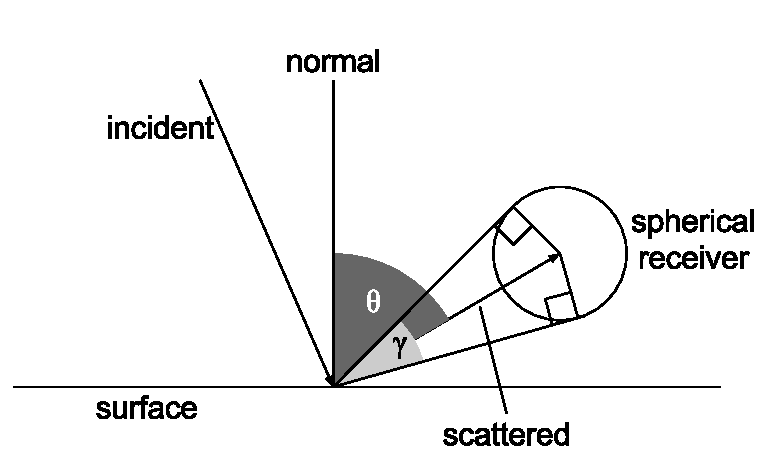
\includegraphics{images/diffuse_rain.pdf}
\caption{Angles used in the diffuse rain equation for a spherical
receiver.\label{fig:diffuse_rain}}
\end{figure}

\section{DWM Implementation}\label{dwm-implementation-1}

\subsection{Possible Methods}\label{possible-methods}

Two methods from the literature were considered for use in Wayverb. A
brief overview of each will be given here.

\subsubsection{KW-Pipe Technique}\label{kw-pipe-technique}

This method is described in
{[}\protect\hyperlink{ref-murphyux5fkw-boundaryux5f2007}{69}{]} and
{[}\protect\hyperlink{ref-kelloniemiux5ffrequency-dependentux5f2006}{70}{]}.

As described in the
\href{\%7B\%7B\%20site.baseurl\%20\%7D\%7D\%7B\%\%20link\%20waveguide.md\%20\%\%7D}{Digital
Waveguide Mesh} section, there are two technically-equivalent
formulations of digital waveguides meshes, known as \emph{W-models} and
\emph{K-models}. W-models allow for straightforward interaction with a
variety of termination types, such as wave digital filters, which can be
used to model frequency-dependent boundaries and air absorption.
However, W-models use more than twice the memory of the equivalent
K-model {[}\protect\hyperlink{ref-beesonux5froomweaver:ux5f2004}{18}{]}.
For large-scale simulations, K-models are preferable for their reduced
memory usage. However, K-models cannot interact directly with wave
digital filters.

The KW-pipe is a ``converter'' between wave- and Kirchhoff- variables,
which is designed to allow the majority of a model (that is, the
air-filled space inside it) to be constructed as a K-model waveguide
mesh. At the boundaries of the model, the KW-pipe is used to connect
K-model nodes to W-model nodes. These W-model nodes can then be
connected to wave digital filters to simulate frequency-dependent
absorption of wave energy. The complete model retains both the
memory-efficiency of the K-model and the termination flexibility of the
W-model, with the drawback of additional implementation complexity at
the interface between the two model types.

This sounds extremely promising, but has a major drawback, as described
by Kowalczyk and Van Walstijn
{[}\protect\hyperlink{ref-kowalczykux5fmodelingux5f2008}{59}{]}: while
the inside of the mesh will be 2- or 3-dimensional, the boundary
termination afforded by the wave-variable boundary is 1-dimensional.
Each boundary node connects to just the closest interior node. As a
result, the edges and corners are not considered to be part of the
model, as these nodes do not have a directly adjacent interior node.
Additionally, the 1D boundary termination equation implies a smaller
inter-nodal distance than that of the 2D or 3D mesh interior. This means
that when updating an interior node next to a boundary, the inter-nodal
distance is greater than when updating the boundary node itself. For
these reasons, the 1D termination is unphysical and can lead to large
errors in the phase and amplitude of reflections
{[}\protect\hyperlink{ref-kowalczykux5fmodelingux5f2008}{59}{]}.

\subsubsection{Locally Reactive Surfaces
Technique}\label{locally-reactive-surfaces-technique}

This method, described in
{[}\protect\hyperlink{ref-kowalczykux5fmodelingux5f2008}{59}{]}, aims to
create physically correct higher-dimensional boundaries by combining a
boundary condition, defined by a boundary impedance, with the
multidimensional wave equation. This leads to a model for a
\emph{locally reacting surface} (LRS), in which boundary impedance is
represented by an infinite-impulse-response (IIR) filter.

As noted above, a surface is locally reacting if the normal component of
the particle velocity on the boundary surface is dependent solely upon
the sound pressure in front of the boundary. In most physical surfaces,
the velocity at the surface boundary will also be influenced by the
velocity at adjacent points on the boundary, so LRS is not a realistic
physical model in the vast majority of cases.

However, despite that it is not a realistic physical model, the
implementation of the LRS modelling technique is both stable and
accurate, as opposed to the 1D KW-pipe termination, which does not
accurately model even locally-reacting surfaces.

The LRS model leads to an implementation that is efficient (as it is
based completely on the K-model/FDTD formulation) and tunable
(boundaries are defined by arbitrary IIR filters).

\subsection{Choice of Boundary Technique for the
DWM}\label{choice-of-boundary-technique-for-the-dwm}

The LRS technique was chosen, as it represented the best compromise
between memory efficiency, customization and tuning, and realism. The
particular strengths of this model are its performance and tunability,
though as mentioned previously it is not physically accurate in many
cases. That being said, neither of the boundary models considered are
particularly realistic, so even for applications where realism is the
most important consideration, the LRS model seems to be the most
appropriate.

\subsection{LRS Implementation}\label{lrs-implementation}

See {[}\protect\hyperlink{ref-kowalczykux5fmodelingux5f2008}{59}{]} and
{[}\protect\hyperlink{ref-kowalczykux5fmodellingux5f2008}{71}{]} for a
more detailed explanation.

The reflectance of a LRS has been defined above (41), in terms of the
normal-incidence specific impedance \(\xi_0\). For the geometric
implementation, \(\xi_0\) was defined in terms of a single
normal-incidence reflection coefficient \(R_0\) (44). If \(R_0\) is
replaced by a digital filter \(R_0(z)\), then the specific impedance may
also be expressed as a filter \(\xi_0(z)\):

\begin{enumerate}
\def\labelenumi{(\arabic{enumi})}
\setcounter{enumi}{46}
\tightlist
\item
  \[\xi_0(z)=\frac{1+R_0(z)}{1-R_0(z)}\]
\end{enumerate}

To create the filter \(R_0\), per-band normal reflection magnitudes are
found using the relationship \(|R|=\sqrt{1-\alpha}\). Then, the
Yule-Walker method is used to find \emph{infinite impulse response}
(IIR) coefficients for a filter with an approximately-matched frequency
response. Then, this filter is substituted into (47) to find IIR
coefficients for the specific impedance filter. This impedance filter
will eventually be ``embedded'' into the boundary nodes of the
waveguide.

Surfaces with detailed frequency responses will require high-order
filters. This generally leads to numerical instability in IIR filters.
The usual solution to this problem would be to split the high-order
filter into a series-combination of lower-order filters. However, the
LRS requires access to intermediate values from the filter delay-line
which makes this approach impossible. An alternative solution is
suggested in
{[}\protect\hyperlink{ref-oxnardux5ffrequency-dependentux5f2015}{72}{]},
which suggests running the entire simulation multiple times, once for
each octave band. This means that the boundary filters can be
single-order, and resistant to accumulated numerical error. Compared to
high-order boundary filters, this method gives much improved accuracy,
but at the cost of running the entire simulation multiple times. In
Wayverb, both approaches are possible, allowing the user to choose
between a fast, inaccurate single-run simulation with high-order
filters; or a slow, accurate multi-run simulation with low-order
filters.

To implement the waveguide boundaries, the computed impedance filter
coefficients are inserted into three special update equations, which are
found by combining the discrete 3D wave equation with the discrete LRS
boundary condition. These equations are used instead of the standard
update equation when updating the boundary nodes. The exact update
equations have not been reproduced here due to space constraints, but
they can be found in
{[}\protect\hyperlink{ref-kowalczykux5fmodelingux5f2008}{59}{]},
alongside a thorough derivation and explanation. The implementation in
Wayverb does not make any modifications to these equations.

The three different update equations are chosen depending on the
placement of the boundary nodes. In the case of a flat wall, the
boundary node is adjacent to a single inner-node, and a ``1D'' update
equation is used. Where two perpendicular walls meet, the nodes along
the edge will each be adjacent to two ``1D'' nodes, and a ``2D'' update
equation is used for these nodes. Where three walls meet, the corner
node will be directly adjacent to three ``2D'' nodes, and a ``3D''
update equation is used for this node. The three types of boundary nodes
are shown in the following diagram
\text{(\ref{fig:boundary_type_diagram})}. Note that this method is only
capable of modelling mesh-aligned surfaces. Other sloping or curved
surfaces must be approximated as a group of narrow mesh-aligned surfaces
separated by ``steps''. For example, a wall tilted at 45 degrees to the
mesh axes will be approximated as a staircase-like series of ``2D'' edge
nodes.

\begin{figure}[htbp]
\centering
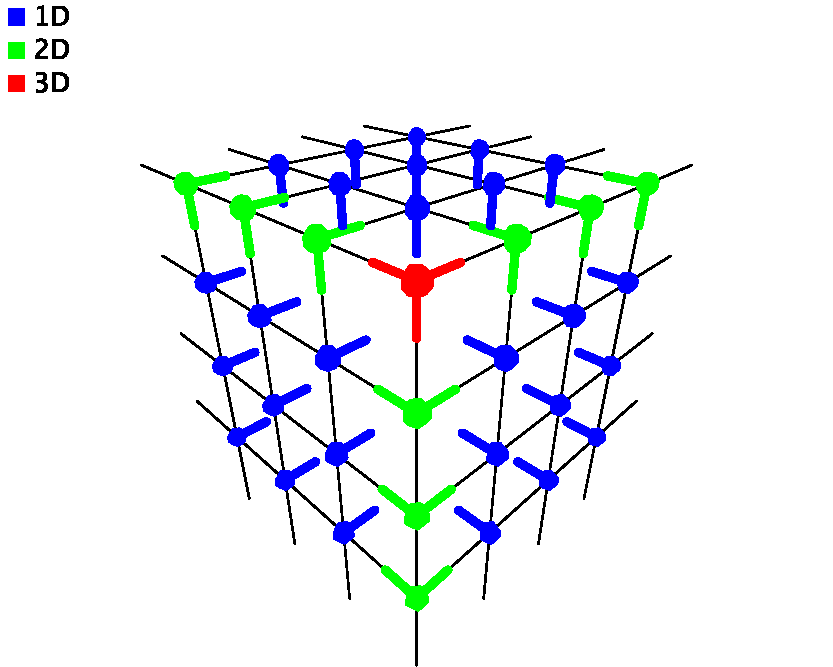
\includegraphics{images/boundary_diagram.pdf}
\caption{The three types of boundary nodes, used to model reflective
planes, edges, and corners. 1D nodes are adjacent to inner nodes, 2D
nodes are adjacent to two 1D nodes, and 3D nodes are adjacent to three
2D nodes.\label{fig:boundary_type_diagram}}
\end{figure}

\section{Testing of the LRS Boundary for the
DWM}\label{testing-of-the-lrs-boundary-for-the-dwm}

The LRS waveguide boundary is complex to implement, as it embeds IIR
filters into the waveguide boundaries, so it is worth ensuring that the
boundary nodes behave as expected.

Although the 3D boundary equations are presented in
{[}\protect\hyperlink{ref-kowalczykux5fmodelingux5f2008}{59}{]}, only 2D
boundaries are tested. Therefore the test shown in this thesis is a
novel contribution, as no previous empirical evidence exists for the 3D
LRS boundary implementation in the waveguide mesh. The test used here is
an extension of the test procedure presented in
{[}\protect\hyperlink{ref-kowalczykux5fmodelingux5f2008}{59}{]}, but
extended to three dimensions.

\subsection{Method}\label{method-1}

A mesh with dimensions \(300 \times 300 \times 300\) nodes, and a
sampling frequency of 8KHz, was set up. A source and receiver were
placed at a distance of 37 node-spacings from the centre of one wall.
The source position was dictated by an azimuth and elevation relative to
the centre of the wall, with the receiver placed directly in the
specular reflection path. The simulation was run for 420 steps. The
first output, \(r_f\), contained a direct and a reflected response.
Then, the room was doubled in size along the plane of the wall being
tested. The simulation was run again, recording just the direct response
at the receiver (\(r_d\)). Finally, the receiver position was reflected
in the boundary under test, and the simulation was run once more,
producing a free-field response (\(r_i\)). The following diagram
\text{(\ref{fig:boundary_test_setup})} shows the testing setup.

\begin{figure}[htbp]
\centering
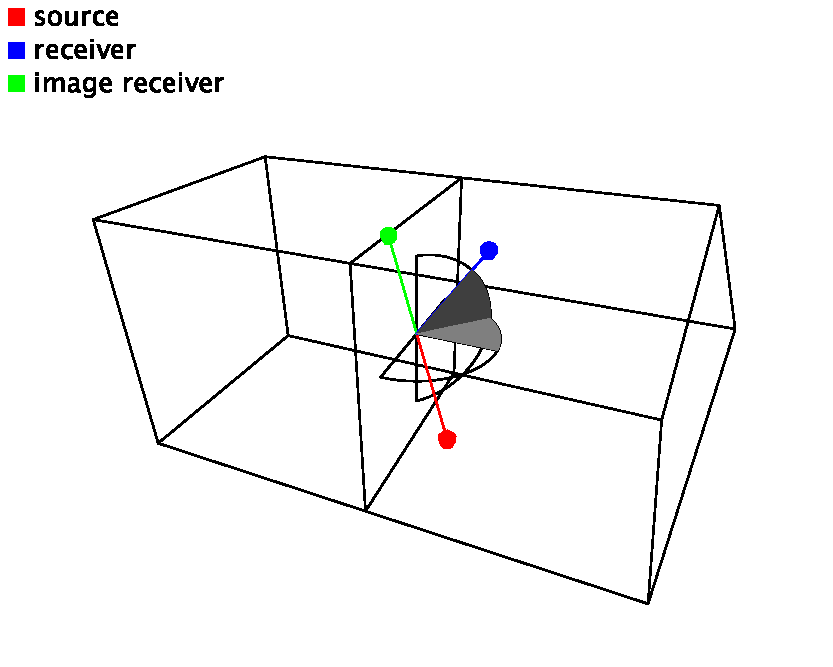
\includegraphics{images/boundary_testing_setup.pdf}
\caption{The setup of the two room-sizes, and the positions of sources
and receivers inside.\label{fig:boundary_test_setup}}
\end{figure}

The reflected response was isolated by subtracting \(r_d\) from \(r_f\),
cancelling out the direct response. This isolated reflection is \(r_r\).
To find the effect of the frequency-dependent boundary, the frequency
content of the reflected response was compared to the free-field
response \(r_i\). This was achieved by windowing \(r_r\) and \(r_i\)
with the right half of a Hann window, then taking FFTs of each. The
experimentally determined numerical reflectance was determined by
dividing the magnitude values of the two FFTs.

To find the accuracy of the boundary model, the numerical reflectance
was compared to the theoretical reflection of the digital impedance
filter being tested, which is defined as:

\begin{enumerate}
\def\labelenumi{(\arabic{enumi})}
\setcounter{enumi}{47}
\tightlist
\item
  \[R_{\theta, \phi}(z) = \frac{\xi(z)\cos\theta\cos\phi -
  1}{\xi(z)\cos\theta\cos\phi + 1}\]
\end{enumerate}

where \(\theta\) and \(\phi\) are the reflection azimuth and elevation
respectively.

The test was run for three different angles of incidence, with matched
azimuth and elevation angles of 0, 30, and 60 degrees respectively.
Three different sets of surface absorption coefficients were used,
giving a total of nine combinations of source position and absorption
coefficients. The specific absorption coefficients are those suggested
in
{[}\protect\hyperlink{ref-oxnardux5ffrequency-dependentux5f2015}{72}{]},
shown in the following table:

\begin{table}[ht]
\centering

\caption{}

\begin{tabular}{@{}llllll@{}}
\toprule

band centre frequency / Hz & 31 & 73 & 173 & 411 & 974 \\\midrule

plaster & 0.08 & 0.08 & 0.2 & 0.5 & 0.4 \\
wood & 0.15 & 0.15 & 0.11 & 0.1 & 0.07 \\
concrete & 0.02 & 0.02 & 0.03 & 0.03 & 0.03 \\

\bottomrule
\end{tabular}

\end{table}

The boundary filter for each material was generated by converting the
absorption coefficients to per-band reflectance coefficients using the
relationship \(R=\sqrt{1-\alpha}\). Then, the Yule-Walker method from
the ITPP library {[}\protect\hyperlink{ref-ux5fitppux5f2013}{73}{]} was
used to calculate coefficients for a sixth-order IIR filter which
approximated the per-band reflectance. This filter was converted to an
impedance filter by \(\xi(z)=\frac{1+R_0(z)}{1-R_0(z)}\), which was then
used in the boundary update equations for the DWM.

\subsection{Results}\label{results}

The results are shown in the following figure
\text{(\ref{fig:reflectance})}. Although the waveguide mesh has a
theoretical upper frequency limit of 0.25 of the mesh sampling rate, the
3D FDTD scheme has a cutoff frequency of 0.196 of the mesh sampling rate
for axial directions. This point has been marked as a vertical line on
the result graphs.

\begin{figure}[htbp]
\centering
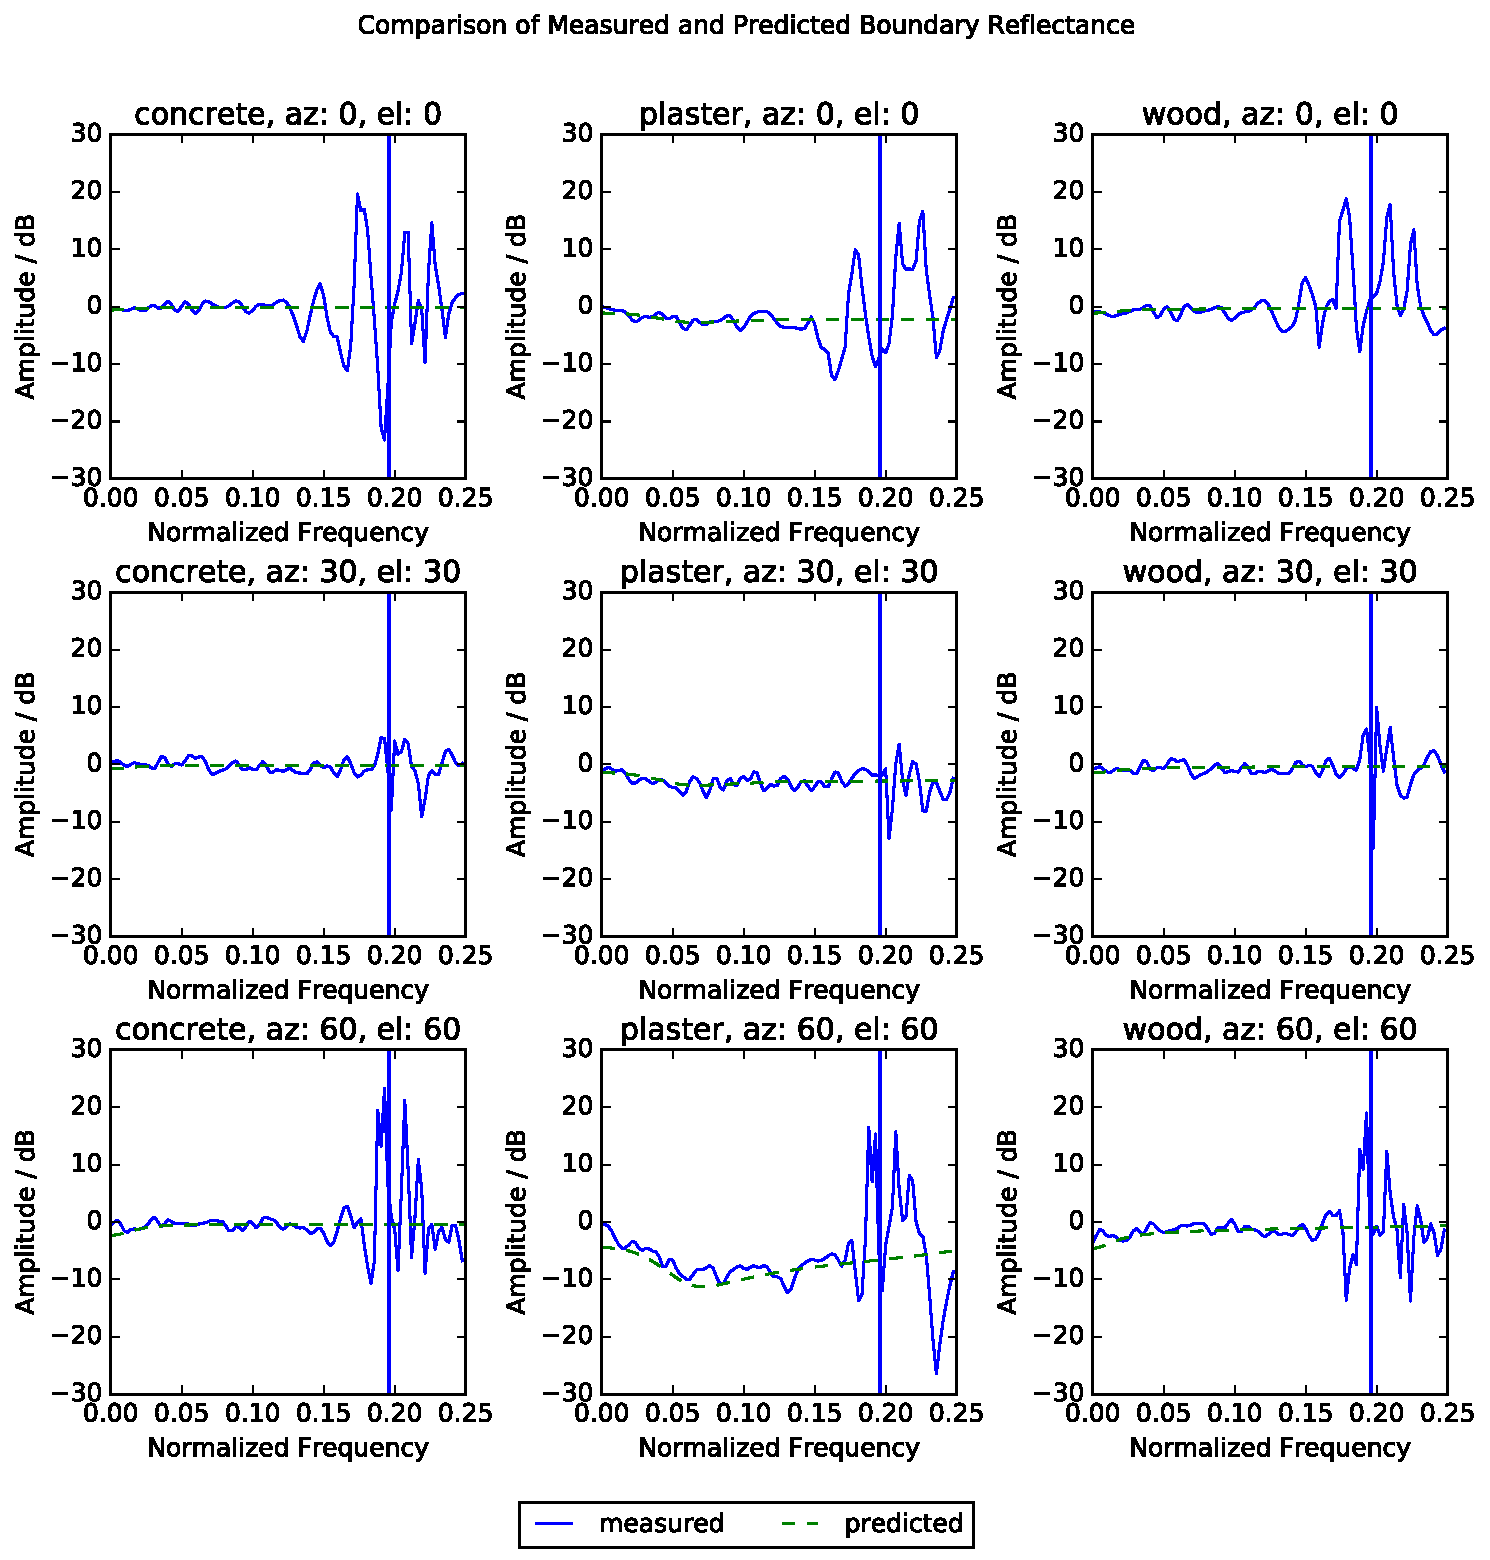
\includegraphics{images/reflectance.pdf}
\caption{Measured boundary reflectance is compared against the predicted
reflectance, for three different materials and three different angles of
incidence.\label{fig:reflectance}}
\end{figure}

\subsection{Evaluation}\label{evaluation}

The initial impression of the results is that the measured response is
reasonably accurate, to within 6dB of the predicted response, but only
below 0.15 of the mesh sampling rate. Above this point, the responses
become very erratic, with very large peaks and troughs. This is
especially true for the on-axis (0-degree) tests, where some erratic
behaviour is seen as low as 0.12 of the mesh sampling rate. This may be
due to numerical dispersion in the waveguide mesh, which is greatest
along axial directions
{[}\protect\hyperlink{ref-kowalczykux5fmodelingux5f2008}{59}{]}. At the
low end of the spectrum, the results look acceptable, adhering closely
to the predicted response.

The poor performance at the top of the spectrum is not particularly
concerning, as the waveguide mesh is designed to generate low-frequency
content. If wideband results are required, then the mesh can simply be
oversampled. To prevent boundary modelling error affecting the results
of impulse response synthesis in the Wayverb app, the mesh cutoff
frequency is locked to a maximum of 0.15 of the mesh sampling rate.

Ideally, these tests would be carried out using flat wave-fronts.
Kowalczyk and Van Walstijn note that some of their results display
low-frequency artefacts because the simulated wave-front is not
perfectly flat. However, flat wave-fronts are not easily accomplished.
The experiments in
{[}\protect\hyperlink{ref-kowalczykux5fmodelingux5f2008}{59}{]} use
large meshes (around 3000 by 3000 nodes, nine million in total) and
place the sources a great distance away from the boundary being studied
in order to maintain a mostly-flat wave-front. This is only practical
because the experiments are run in two dimensions. For the 3D case, no
experimental results are given. This is probably because running a 3D
simulation on a similar scale would require a mesh of twenty-seven
billion nodes, which in turn would require gigabytes of memory and hours
of simulation time.

There is little low-frequency error in the experimental results above,
despite the fact that the source is placed very close to the boundary,
and the wave-front is therefore very rounded. This rounded wave-front
may, however, be the cause of the relatively small broadband
fluctuations between 0 and 0.15 of the mesh sampling rate. The filters
used in this test are also of much higher order than those tested in
{[}\protect\hyperlink{ref-kowalczykux5fmodelingux5f2008}{59}{]}, giving
a greater chance of accumulated numerical error. This may be the cause
of the volatile high-frequency behaviour.

In conclusion, for the most part, the results presented adhere closely
to the expected results, with the caveat that the surface reflectance is
only accurate at low frequencies, below around 0.15 of the mesh sampling
rate. Different absorption coefficients lead to clearly-different
reflectance coefficients, which are additionally accurate at multiple
angles of incidence. Whilst a more accurate method would be preferable,
this model is both fast and tunable, making it a good candidate for
boundary modelling in room acoustics simulations.

\chapter{Evaluation}\label{evaluation-1}

This section describes the Wayverb program, and demonstrates some
example simulation results. The simulations are chosen to highlight the
behaviour of the simulator with respect to parameters such as reverb
time, frequency content, and early reflection times. The project files
for each of these tests is included in the Wayverb distribution.

\section{Features}\label{features}

The Wayverb program has the following features:

\begin{itemize}
\tightlist
\item
  \textbf{Hybrid Geometric and Waveguide Simulation}: This is the most
  important feature of Wayverb, providing the ability to simulate the
  acoustics of arbitrary enclosed spaces.
\item
  \textbf{Load Arbitrary Models}: The model-importing functionality is
  built on top of the Assimp library, which has support for a wide
  variety of 3D formats
  {[}\protect\hyperlink{ref-ux5fassimpux5f2017}{74}{]}. Care must be
  taken to export models with the correct scale, as Wayverb interprets
  model units as metres. The detected model dimensions are shown in the
  interface, so that model dimensions can be checked, and the model can
  be re-exported if necessary.
\item
  \textbf{Visualiser}: Allows the state of the simulation to be
  observed, as it changes.
\item
  \textbf{Unlimited Sources and Receivers}: Set up any number of sources
  and receivers. This has the trade-off that the simulation will
  automatically run once for each source-receiver pair, which will be
  time consuming when there are many combinations.
\item
  \textbf{Multiple Capsules per Receiver}: Each receiver behaves like a
  set of coincident capsules. Each capsule may model an ideal
  microphone, or an HRTF ear. Multiple capsules at the same receiver
  require only a single simulation run, so multi-capsule receivers
  should be preferred over multiple receivers, wherever possible. For
  HRTF simulations, the receiver position will be automatically adjusted
  during the image-source simulation, replicating the interaural spacing
  of a real pair of ears (see the Image Source Implementation subsection
  of the
  \href{\%7B\%7B\%20site.baseurl\%20\%7D\%7D\%7B\%\%20link\%20microphone.md\%20\%\%7D}{Microphone
  Modelling} section). This produces a realistic stereo time-delay
  effect in the early-reflection portion of the output, aiding
  localisation.
\item
  \textbf{Custom Materials}: Wayverb reads unique material names from
  the loaded 3D model. Each unique material in the model may be assigned
  custom acoustic properties, consisting of multi-band absorption and
  scattering coefficients.
\item
  \textbf{Tunable Ray Tracer}: The number of rays is controlled by a
  quality parameter, which defines the number of rays which are expected
  to intersect the receiver per histogram interval. Higher quality
  values will lead to more accurate reverb tails, at the cost of longer
  processing times. The desired image-source depth can also be varied
  from 0 to 10, although lower values are recommended. In the real
  world, the ratio of scattered to non-scattered sound energy will
  increase as the impulse response progresses. The image-source model
  does not account for scattering. Therefore, lower image-source
  reflection depths are more physically plausible, as the simulation
  will switch to stochastic ray-tracing (which \emph{does} account for
  scattering) sooner.
\item
  \textbf{Tunable Waveguide}: The waveguide has two modes: a single-band
  mode which uses the Yule-Walker method to estimate boundary filter
  parameters, and a multi-band mode which uses ``flat'' filters. These
  filters are able to model a given wall absorption with greater
  accuracy, but only when the wall absorption is constant across the
  spectrum. The multi-band mode is therefore significantly slower, as it
  must run the waveguide process several times. It uses the wall
  absorption from each frequency band in turn, and then band-pass
  filters and mixes the results of each simulation to find the final
  output. Both waveguide modes allow the maximum waveguide frequency,
  and the oversampling factor, to be modified.
\end{itemize}

The interface of the Wayverb program is explained in the following
figure\text{
(\ref{fig:wayverb_ui})}.

\begin{figure}[htbp]
\centering
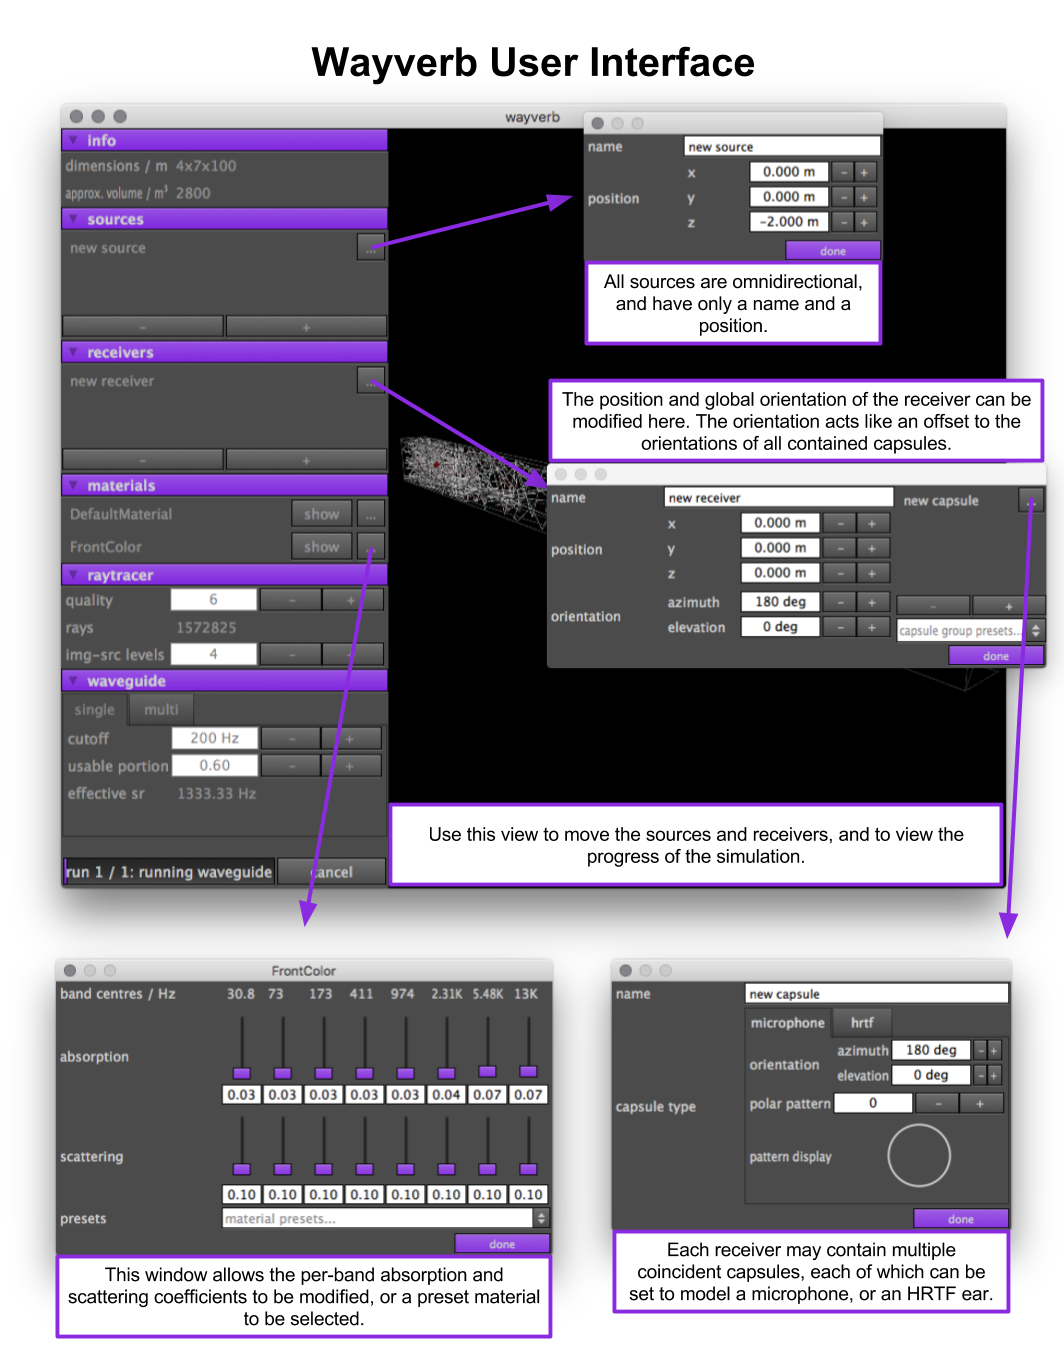
\includegraphics{images/wayverb_ui.pdf}
\caption{The interface of the Wayverb program.\label{fig:wayverb_ui}}
\end{figure}

\section{Tests}\label{tests}

Some aspects of the Wayverb algorithm have already been tested in
previous sections, and so do not require further testing here.

Specifically, the
\href{\%7B\%7B\%20site.baseurl\%20\%7D\%7D\%7B\%\%20link\%20hybrid.md\%20\%\%7D}{Hybrid
Model} section compares the waveguide to an ideal image-source model,
showing that the output level is correctly matched between models. This
test also shows that the modal response of the waveguide matches the
``ideal'' response for several different values of absorption
coefficients, implying that the waveguide and image-source boundary
models are consistent.

The
\href{\%7B\%7B\%20site.baseurl\%20\%7D\%7D\%7B\%\%20link\%20microphone.md\%20\%\%7D}{Microphone
Modelling} section shows that the waveguide model is capable of
simulating directionally-dependent receivers, with gain dependent on the
angle of the incident wave-front.

Finally, the
\href{\%7B\%7B\%20site.baseurl\%20\%7D\%7D\%7B\%\%20link\%20boundary.md\%20\%\%7D}{Boundary
Modelling} section shows that the waveguide boundaries exhibit the
expected wall impedance (though with some error, which increases at
higher frequencies).

In the tests below, all impulse responses are produced using the Wayverb
software. Reverb times are calculated using the Room EQ Wizard
{[}\protect\hyperlink{ref-ux5froomux5f2017}{75}{]}. The test projects
can be found in the Wayverb repository.

\subsection{Terms and Measurements}\label{terms-and-measurements}

Here, reverb times are described using the \emph{RT60}, which is a
parameter denoting the time taken for the sound level in a space to fall
by sixty decibels
{[}\protect\hyperlink{ref-ux5freverberationux5f2017}{76}{]}. Commonly,
impulse response recordings do not have the necessary dynamic range of
75dB or more which is necessary to directly calculate the RT60. Instead,
a smaller level decrease is timed, and this time is extrapolated to give
an estimate of the RT60. The time taken for a twenty or thirty decibel
decrease is used, and multiplied by two or three respectively to
estimate the RT60. These measurements are known as the T20 and T30.

The estimated or predicted RT60, \(T\), of a given space can be
calculated using the Sabine formula
{[}\protect\hyperlink{ref-kuttruffux5froomux5f2009}{29}, p. 131{]}:

\begin{enumerate}
\def\labelenumi{(\arabic{enumi})}
\setcounter{enumi}{48}
\tightlist
\item
  \[T=0.161\frac{V}{A}\]
\end{enumerate}

where \(V\) is the volume of the space in cubic metres, and \(A\) is the
\emph{equivalent absorption area}. The absorption area of a given
surface is equal to the area of the surface multiplied by its absorption
coefficient. The equivalent absorption area for an entire room is found
by summing the absorption areas of all surfaces in the scene.

\subsection{Reverb Times for Varying Room
Volumes}\label{reverb-times-for-varying-room-volumes}

This test aims to check that rooms with different volumes produce the
expected reverb times. Rooms with different volumes, but the same
absorption coefficients and source/receiver positions, are simulated.
Then, the RT60 is calculated from the simulated impulse responses, and
compared against the Sabine estimate. A close match shows that the
change in room volume has the correct, physically plausible effect on
the generated outputs.

Three different cuboid rooms with the following dimensions are modelled:

\begin{itemize}
\tightlist
\item
  \textbf{small}: \(2 \times 2.5 \times 3\) metres
\item
  \textbf{medium}: \(4.5 \times 2.5 \times 3.5\) metres
\item
  \textbf{large}: \(12 \times 4 \times 8\) metres
\end{itemize}

Each room is set to have absorption and scattering coefficients of 0.1
in all bands. The source and receiver are placed 1 metre apart at the
centre of each room. The waveguide is used to model frequencies up to
500Hz, using a mesh with a sampling rate of 3330Hz. The image-source
model generates reflections up to the fourth order.

The following results are found, for the entire (broadband) output:

\begin{table}[ht]
\centering

\caption{}

\begin{tabular}{@{}llll@{}}
\toprule

room & Sabine RT / s & measured T20 / s & measured T30 / s \\\midrule

small & 0.653 & 0.663 & 0.658 \\
medium & 0.887 & 0.897 & 0.903 \\
large & 1.76 & 1.86 & 1.96 \\

\bottomrule
\end{tabular}

\end{table}

The results for small and medium rooms are within 5\% of the expected
reverb time, although the measured T30 of the larger room has an error
of 11\%. Increasing the room volume has the effect of increasing the
reverb time, as expected.

Now, the results are plotted in octave bands\text{ (figure
\ref{fig:room_size_rt30})}. The results in lower bands, which are
modelled by the waveguide, have a significantly shorter reverb time than
the upper bands, which are generated geometrically. The higher bands
have reverb times slightly higher than the Sabine prediction, while the
waveguide-generated bands show much shorter reverb times tails than
expected. The difference in reverb times between the waveguide and
geometric methods also becomes evident when spectrograms are taken of
the impulse responses\text{ (figure
\ref{fig:room_size_spectrograms})}. In all tests, the initial level is
constant across the spectrum, but dies away faster at lower frequencies.
In the medium and large rooms, some resonance at 400Hz is seen towards
the end of the reverb tail, which is probably caused by numerical
dispersion in the waveguide mesh.

In the medium and large tests, the spectrograms appear as though the
low-frequency portion has a longer, rather than a shorter, reverb time.
However, in the large test, the late low-frequency energy has a maximum
of around -100dB, which is 40dB below the level of the initial
contribution. The measured T20 and T30 values do not take this into
account, and instead reflect the fact that the \emph{initial} reverb
decay is faster at low frequencies. The spectrograms show that the
waveguide sometimes resonates for an extended period at low amplitudes.
In effect, the waveguide exhibits a high noise-floor under some
conditions.

\begin{figure}[htbp]
\centering
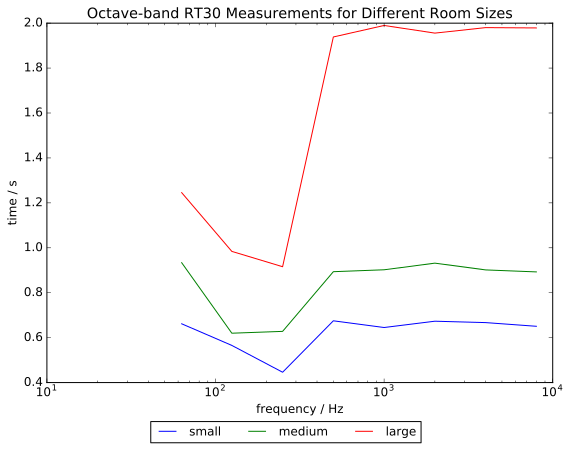
\includegraphics{images/room_size_rt30.pdf}
\caption{T30 in octave bands, calculated from the measured impulse
responses.\label{fig:room_size_rt30}}
\end{figure}

\begin{figure}[htbp]
\centering
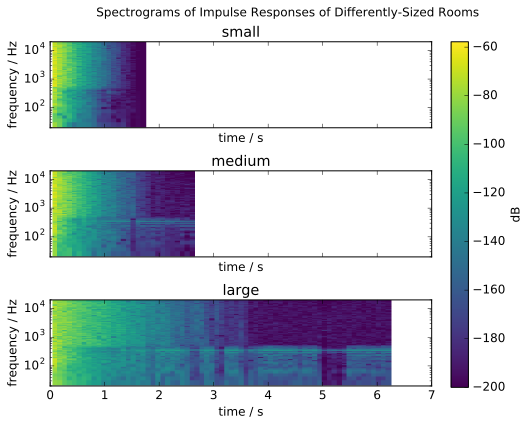
\includegraphics{images/room_size_spectrograms.pdf}
\caption{Spectrograms of impulse responses obtained from different room
sizes.\label{fig:room_size_spectrograms}}
\end{figure}

This result is difficult to explain. A shorter reverb time indicates
that energy is removed from the model at a greater rate than expected.
Energy in the waveguide model is lost only at boundaries, so the most
likely explanation is that these boundaries are too absorbent. It is
also possible that the microphone model causes additional unexpected
attenuation.

Further tests (not shown) of the three rooms were carried out to check
possible causes of error. In one test, the Yule-Walker-generated
boundary filters were placed with filters representing a constant
real-valued impedance across the spectrum, to check whether the boundary
filters had been generated incorrectly. In a second test, the modelled
omnidirectional microphone at the receiver was removed, and the raw
pressure value at the output node was used instead, to check that the
microphone was not introducing undesired additional attenuation.
However, in both tests, similar results were produced, with reverb times
significantly lower than the Sabine prediction. The boundary and
microphone models do not appear to be the cause of the problem.

The reverb-time test at the end of the
\href{\%7B\%7B\%20site.baseurl\%20\%7D\%7D\%7B\%\%20link\%20hybrid.md\%20\%\%7D}{Hybrid
Model} section shows that the waveguide reverb times match the reverb
times of the exact image-source model, which will be close to the
analytical solution in a cuboid room. The close match to the
almost-exact image-source model suggests that the waveguide and boundary
model have been implemented correctly. Additionally, the tests in the
\href{\%7B\%7B\%20site.baseurl\%20\%7D\%7D\%7B\%\%20link\%20boundary.md\%20\%\%7D}{Boundary
Modelling} section show that wall impedances are accurately modelled.

Given that in all previous tests the waveguide behaves as expected, one
possibility is that the Sabine equation is simply a poor predictor of
low-frequency reverb times, or reverb times in regularly-shaped rooms
with well-defined reflection patterns (such as cuboids). If this were
the case, this might justify the waveguide results. This is a reasonable
suggestion: the Sabine equation assumes that the sound field is diffuse,
which in turn requires that at any position within the room, reverberant
sound has equal intensity in all directions, and random phase relations
{[}\protect\hyperlink{ref-hodgsonux5fwhenux5f1994}{77}{]}. This is
obviously untrue in a cuboid at low frequencies, where the non-random
phase of reflected waves causes strong modal behaviour due to waves
resonating between the parallel walls of the enclosure.

Further testing is required to locate the exact cause of the differences
in reverb times. In the present implementation, the mismatch is an
obvious artefact in the output, which affects the impulse response's
suitability for musical applications.

\subsection{Reverb Times for Varying
Absorptions}\label{reverb-times-for-varying-absorptions}

This test simulates the same room with several different absorption
coefficients. The ``medium'' room from the above test is simulated,
again with the source and receiver placed 1 metre apart in the centre of
the room. Scattering is set to 0.1 in all bands. The absorption
coefficients are set to 0.02, 0.04, and 0.08, corresponding to Sabine
predictions of 4.43, 2.22, and 1.11 seconds.

\begin{table}[ht]
\centering

\caption{}

\begin{tabular}{@{}llll@{}}
\toprule

absorption & Sabine RT / s & measured T20 / s & measured T30 /
s \\\midrule

0.02 & 4.433 & 4.295 & 4.283 \\
0.04 & 2.217 & 2.210 & 2.219 \\
0.08 & 1.108 & 1.126 & 1.156 \\

\bottomrule
\end{tabular}

\end{table}

The issue with shorter low-frequency decay times persists in this test.
However, the broadband reverb time responds correctly to the change in
absorption coefficients.

\begin{figure}[htbp]
\centering
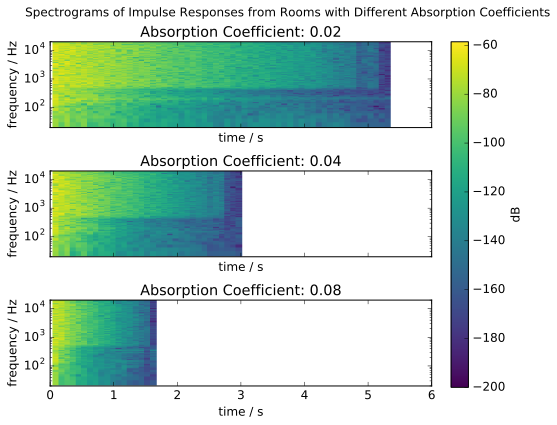
\includegraphics{images/room_material_spectrograms.pdf}
\caption{Spectrograms of impulse responses obtained from simulating the
same room with different absorption coefficients. Note that the
low-frequency content has a shorter decay time than the high-frequency
content.\label{fig:room_material_spectrograms}}
\end{figure}

\subsection{Direct Response Time}\label{direct-response-time}

The ``large'' room above is simulated again, but with the source and
receiver positioned in diagonally opposite corners, both 1 metre away
from the closest walls in all directions. The generated impulse response
is compared to the previous impulse response, in which the source and
receiver are placed 1 metre apart in the centre of the room.

Sound is simulated to travel at 340m/s, so when the source and receiver
are placed 1m apart, a strong impulse is expected after 1/340 = 0.00294
seconds. In the new simulation, the source and receiver are placed
\(\sqrt{10^2 + 2^2 + 6^2}\) = 11.8m apart, corresponding to a direct
contribution after 0.0348 seconds.

When the source is further away, the direct contribution may not be the
loudest part of the impulse. As the distance from the source \(r\)
increases, the energy density of the direct component decreases
proportionally to \(1/r^2\). However, the energy density in an
ideally-diffuse room is independent of \(r\). At a certain distance,
known as the \emph{critical distance} \(r_c\), the energy densities of
the direct component and reverberant field will match. Beyond the
critical distance, the energy of the direct component will continue to
decrease relative to the reverberant field
{[}\protect\hyperlink{ref-kuttruffux5froomux5f2009}{29}, pp.
146--147{]}.

This effect is observed for the larger separating distance. The first
and second order early reflections arrive very shortly after the direct
response. Many of these reflection paths cover the same distance, and so
arrive at the same time. These contributions are added, giving an
instantaneous energy which is often greater than that of the direct
contribution. The early reflections also occur at a greater frequency
for the increased spacing. Therefore it is obvious that the ratio of
energy densities between the direct and reverberant contributions is
lower for greater spacings, as expected.

\begin{figure}[htbp]
\centering
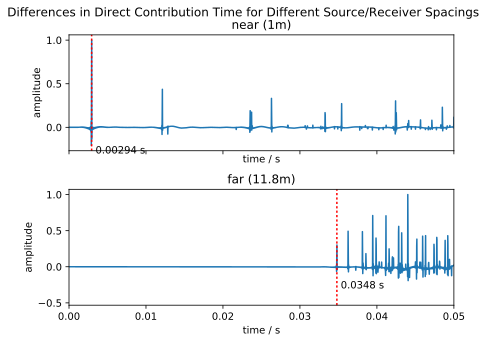
\includegraphics{images/spacing_signals.pdf}
\caption{Larger distances between the source and receiver result in
delayed initial contributions. This figure shows the first 0.05s of the
outputs of two simulations in which the source and receiver are
separated by 1m and 11.8m.\label{fig:spacing_signals}}
\end{figure}

\subsection{Obstructions}\label{obstructions}

Early reflection behaviour seems to be correct in simple cuboid models,
where there is always line-of-sight between the source and receiver. The
behaviour in more complex models, in which the source and receiver are
not directly visible, must be checked.

The simulated space is a simple vault-like model, similar to a small
hall, but broken up by regularly repeating pillars. The source and
receiver are positioned seven metres apart, with their view obstructed
by two pillars. If there were no obstruction, a strong direct impulse
would be expected after 0.0206 seconds. However, the pillars should
block this direct contribution.

\begin{figure}[htbp]
\centering
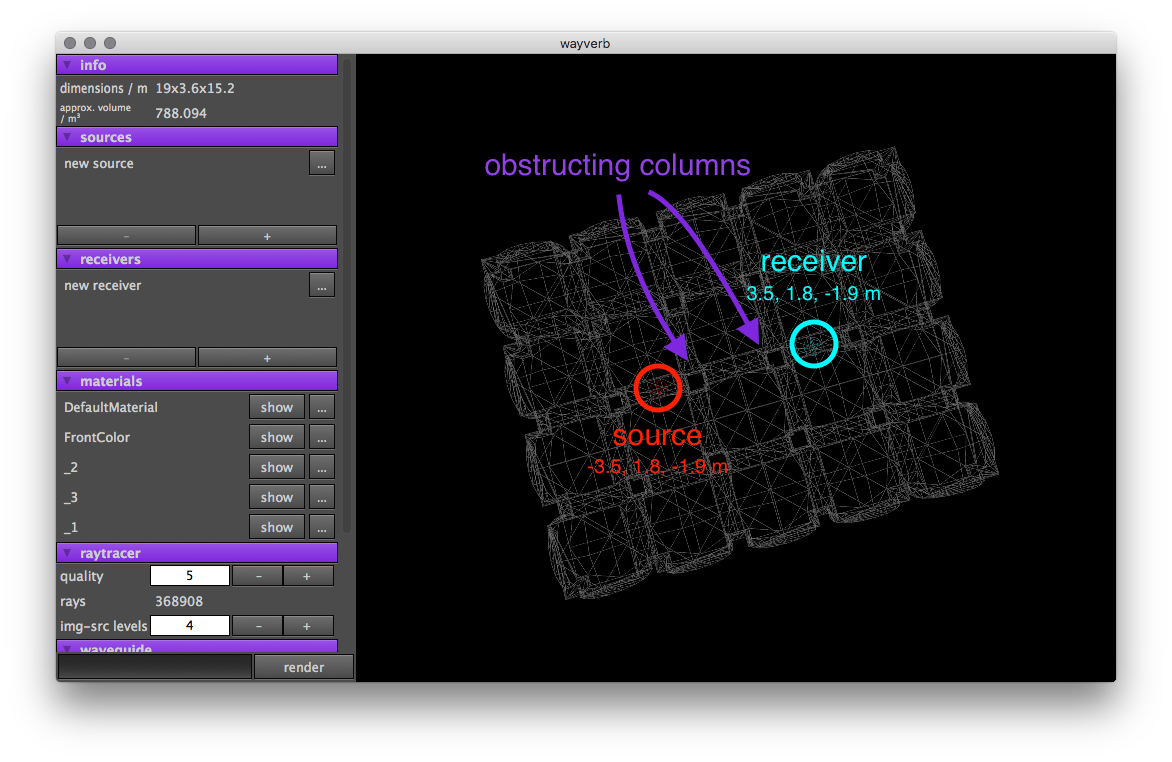
\includegraphics{images/vault_demo.png}
\caption{The testing set-up, showing the pillars blocking the
line-of-sight between the source and receiver.}
\end{figure}

In the real world, objects with areas of a similar or greater order to
the incident wavelength cause diffraction effects
{[}\protect\hyperlink{ref-kuttruffux5froomux5f2009}{29}, p. 59{]}. The
result of diffraction is that an additional ``diffraction wave'' is
created at the edge of the object, which radiates in all directions. In
the vault model, the edges of the pillars should cause diffraction, and
in this way, some energy should be scattered from the source to the
receiver. This energy will arrive slightly after the direct contribution
would have, but before the first early reflection. The shortest possible
path from source to receiver which travels around the pillars has a
length of 7.12m, corresponding to a time of 0.0209s. Though the
image-source and ray tracing models are not capable of modelling
diffraction effects, the waveguide model inherently models this
phenomenon. Therefore, the impulse response should record a
low-frequency excitation at around 0.0209s.

\begin{figure}[htbp]
\centering
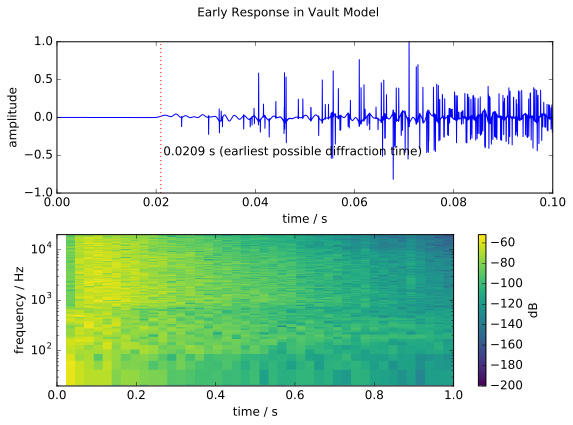
\includegraphics{images/vault_response.pdf}
\caption{The early part of the vault impulse response. Low frequency
diffraction from the waveguide is detected before the first image-source
contribution.\label{fig:vault_response}}
\end{figure}

The impulse response graph \text{(figure \ref{fig:vault_response})}
shows that low frequency diffraction is in fact recorded. Though this
behaviour is physically correct, it highlights the main shortcoming of
the hybrid algorithm. The correct behaviour of the waveguide conflicts
with the approximate nature of the geometric algorithms, causing an
obvious divide or disconnect between the low and high frequency regions
in the output. The low frequencies have a fast onset and immediate
decay, whereas the higher frequencies have a delayed onset with extended
decay. This result is physically implausible, and makes the impulse
response unsuitable for realistic, high-quality reverb effects.

\subsection{Late Reflection Details}\label{late-reflection-details}

Having checked the behaviour of early reflections, now the
late-reflection performance must be checked. The nature of the ray
tracing process means that fine detail (below 1ms precision) is not
captured. However, it should be possible to observe reverb features on a
larger scale, such as distinct echoes from a long tunnel.

A cuboid with dimensions \(4 \times 7 \times 100\) metres is simulated.
The receiver is placed exactly at the centre of the model, with the
source positioned two metres away along the z direction. The output
should contain a direct contribution at 0.00588s, and some early
reflections from the nearby walls. The reverb tail should contain strong
echoes every 0.294s, as the initial wave-front reflects back-and-forth
between the two end walls.

The tunnel is modelled using absorption coefficients of 0.03 in the
bottom five bands, then 0.04, and 0.07 in the highest two bands. The
scattering coefficients are set to 0.1 in all bands. This scattering
should cause echoes in the reverb tail to be ``smeared'' in time. To
check the effect of the scattering coefficients, the same test is also
run using scattering coefficients of 0 in all bands.

\begin{figure}[htbp]
\centering
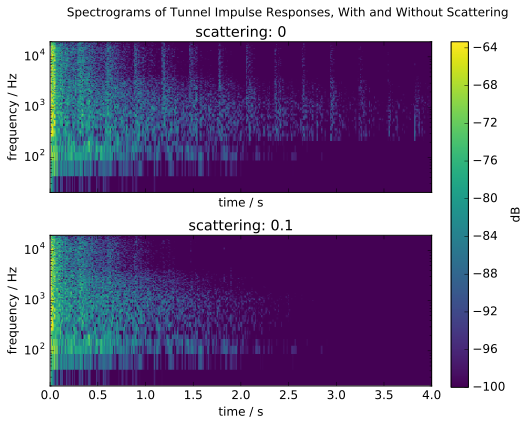
\includegraphics{images/tunnel_spectrograms.pdf}
\caption{Spectrograms of the tunnel impulse responses with different
scattering levels. Note that the first 3 echoes are clear in both
responses, but the scattered response quickly becomes less distinct,
while the response with no scattering has clear echoes which die away
more slowly.\label{fig:tunnel_spectrograms}}
\end{figure}

The spectrograms show that there are clear increases in recorded energy,
occurring approximately every 0.3 seconds after the initial onset. Each
echo is followed by its own decay tail. In the case of the
non-scattering simulation, the echoes are clearly separated, with very
short tails. When the scattering is increased, the tails become longer,
and the individual echoes become less defined. This is expected: when
there is no scattering, rays travelling in any direction other than
along the length of the tunnel will bounce between the walls many times,
attenuated each time. These contributions may arrive at any time at the
receiver, however, their amplitude will be greatly reduced. The rays
travelling directly between the ends of the tunnel will be reflected
fewer times, will lose less energy, and will produce louder regular
contributions. When scattering is introduced, the ray paths are less
regular, giving less correlation between the number of reflections and
the time at which the ray is recorded. This in turn leads to a more even
distribution of recorded energy over time.

\subsection{Directional Contributions}\label{directional-contributions}

To test that microphone modelling behaves as expected, a cardioid
microphone is placed in the exact centre of the ``large'' cuboid room,
facing away from the source, which is positioned at a distance of 3m
along the z-axis.

An ideal cardioid microphone has unity gain in its forward direction,
and completely rejects waves incident from behind. In this test, the
direct contribution from the source originates directly behind the
receiver, so it should not be present in the output. The first
contribution detected by the receiver is caused by reflections from the
floor and ceiling. Both of these reflection paths have lengths of
exactly 5m, corresponding to 0.0147s. These contributions will be
incident from behind the microphone (but not directly behind) so they
should have a relatively reduced magnitude.

The first contributions that strike the receiver from the front have
path lengths of 11m and 13m, which should correspond to strong impulses
at 0.0324s and 0.0382s.

These expectations are reflected in the results, shown in the following
figure\text{ (\ref{fig:cardioid})}. The impulse response is silent at
the time of the direct contribution, 0.00882s. The first significant
level is recorded at 0.0147s, with the loudest contributions seen at
0.0324s and 0.0382s. These results are consistent across the spectrum,
indicating that the microphone model is matched between both simulation
methods.

\begin{figure}[htbp]
\centering
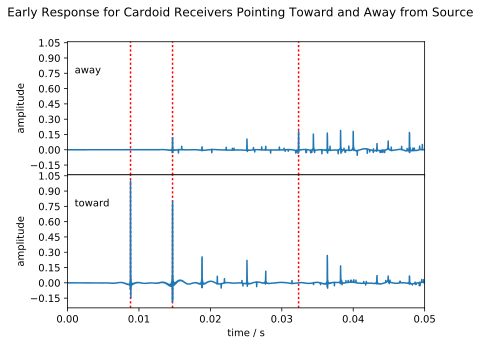
\includegraphics{images/cardioid.pdf}
\caption{The response measured at a cardioid microphone pointing away
from the source. The times marked, from left to right, are the direct
contribution time, the first reflection time, and the first and second
\emph{forward-incident} reflection times.\label{fig:cardioid}}
\end{figure}

\subsection{Binaural Modelling}\label{binaural-modelling}

Finally, the binaural model is tested. A concert hall is simulated, with
a source placed in the centre of the stage area. A receiver is placed
10m away along both the x- and z-axes. The receiver is oriented so that
it is facing directly down the z axis, meaning that the source is 14.1m
away, on the left of the receiver.

The simulation produces output impulse responses for both the left and
right ears. All of Wayverb's simulation methods (image-source,
ray-tracing and waveguide) use HRTF data to produce stereo effects based
on interaural level difference. The image-source method additionally
offsets the receiver position to produce interaural time difference
effects, so in the outputs, slight time differences in the early
reflections between channels are expected, and small level differences
should be seen throughout both files.

In particular, the direct contribution would normally arrive at
14.1/340=0.0416s. However, the left ``ear'' is actually slightly closer
to the source, and the right ear is slightly further away, which means
that the first contribution should be at 0.0414s in the left channel,
and 0.0418s in the right. The right ear is obstructed by the listener's
head, and should therefore have a reduced level relative to the left
ear.

\begin{figure}[htbp]
\centering
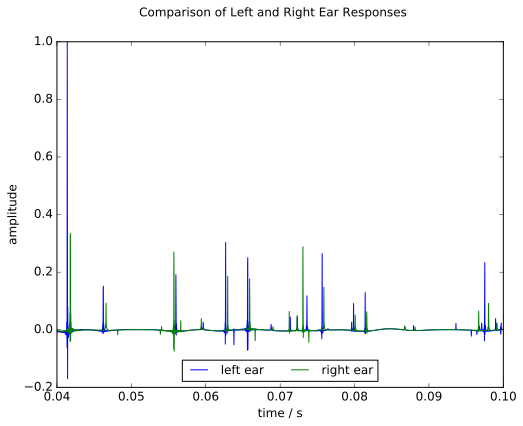
\includegraphics{images/binaural_signals.pdf}
\caption{Comparison of left- and right-ear responses, when the source is
placed to the left of the receiver. Note the amplitude and time
differences between the early reflections. The first contribution, in
particular, is quieter in the right ear because it is occluded by the
listener's virtual head.}
\end{figure}

The expected behaviour is observed in the outputs. The earliest
contribution in the left channel occurs at 0.0414s, and has a greater
level than the right channel's contribution at 0.148s. The left-channel
early reflections have an overall higher level than the early
reflections in the right channel. However, as the impulse response
progresses and becomes more diffuse, the energy levels equalise between
channels.

\section{Analysis}\label{analysis}

\subsection{Simulation Method}\label{simulation-method}

All models perform as expected with regards to changes in room size and
shape, material coefficients, source and receiver positions, and
receiver microphone type. Reverb features such as distinct late echoes
can be generated, and precise stereo effects, relying on both interaural
time- and level-difference, can be created.

The main drawback, evident in several of the tests, is that the
geometric and wave-based models have distinct behaviours. In the
room-size and material tests, there are markedly different reverb times
between the ray-tracer and waveguide outputs; and in the obstruction
test, the waveguide exhibits diffraction behaviour which is not mirrored
in the geometric output. These differences lead to obvious
discontinuities in the frequency response, which persist despite
calibrating the models to produce the same sound level at the same
distance, and implementing matching boundary models in all models.

Some differences are to be expected. The primary reason for implementing
multiple simulation methods is the relative accuracy of the different
methods. Geometric algorithms are known to be inaccurate at low
frequencies, a shortcoming that the waveguide was designed to overcome.

However, an accurate low-frequency response is useless if there is an
obvious disconnect between high- and low-frequency outputs. For music
and sound design applications, responses will sound \emph{more}
artificial if there is a rapid change in the frequency response, even if
the low-frequency response taken alone is an accurate representation of
the modelled space. Here, it is preferable that the frequency response
not contain obvious discontinuities, even if this necessitates a
reduction in overall accuracy.

Practical solutions to this problem are unclear. Ideally, the entire
simulation would be run with the waveguide method, but this is
impractical for all but the smallest simulations. Another option is to
reduce the audible impact of the crossover between the waveguide and
geometric outputs, simply by increasing its width. This has the dual
drawbacks of decreasing the low-frequency accuracy, while also requiring
a higher waveguide sample-rate, which is computationally expensive.
Alternatively, the geometric algorithms may be altered, to account for
effects such as diffraction, with the goal of minimising the differences
between the wave and ray-based methods. This solution would maintain (or
even improve) the accuracy of the simulation, but would again increase
its cost. Finally, the goal of low-frequency accuracy could be
abandoned, and the entire spectrum modelled using geometric methods.
However, this would prevent important characteristics such as modal
behaviour from being recorded.

\subsection{General Implementation}\label{general-implementation}

The implementation has several known issues, other than those shown in
the tests above. These issues can broadly be separated into two
categories: firstly, problems with the simulation algorithm which were
not highlighted in the above tests; and secondly, usability issues with
the program interface.

\subsubsection{Algorithm}\label{algorithm}

As noted in the
\href{\%7B\%7B\%20site.baseurl\%20\%7D\%7D\%7B\%\%20link\%20waveguide.md\%20\%\%7D}{Digital
Waveguide Mesh} section, the input signal used to excite the waveguide
is not optimal. Its frequency response extends up to the Nyquist
frequency, which means that the mesh has energy above the desired output
frequency. As shown in the
\href{\%7B\%7B\%20site.baseurl\%20\%7D\%7D\%7B\%\%20link\%20boundary.md\%20\%\%7D}{Boundary
Modelling} section, the performance of the boundary filters is often
erratic above 0.15 of the mesh sampling rate, sometimes increasing
rather than reducing gain of incident signals. In combination, the
broadband input signal sometimes causes the reflection filters to
repeatedly amplify high-frequency content in the mesh. This is not
audible in the final results, as the high frequency content is filtered
out. However, it still leads to loss of precision, and sometimes numeric
overflow. This might be solved by high-pass filtering the input signal,
and then deconvolving the mesh output. However, it is not clear how such
a process would interact with the microphone simulation. For example, it
would probably be necessary to record and deconvolve the signals at all
nodes surrounding the output node in order to produce a correct
intensity vector. This would require further development and testing,
for which there was insufficient time during the Wayverb project.

A similar drawback is to do with the low-frequency response of the mesh.
Most input signals cause an increasing DC offset when the mesh uses a
``soft'' input node. To solve this, Wayverb's mesh is excited using a
``hard'' node, which introduces low-frequency oscillations and
reflection artefacts. An important area for future research is the
development of an input signal which can be used in conjunction with a
soft source, which does not cause any DC offset.

An important feature which is not implemented in Wayverb is the
modelling of directional sources. Currently, all modelled sources emit a
single spherical wave-front, which has equal energy in all directions.
Real-world sources such as musical instruments and the human voice are
directional. The ability to model directional sources would allow
musicians and sound designers to create much more realistic and
immersive acoustic simulations.

As well as directional sources, it might be useful to make the
implementation of directional receivers more generic. Specifically, an
ambisonic receiver would be useful, so that simulation results could be
exported for directional processing in dedicated software. This could be
achieved without modifying the geometric microphone model, in which
coincident capsules are well-justified and lead to performance
improvements (the simulation is run once for the entire capsule group,
instead of once per individual capsule). However, the approach is not
strictly justified in combination with the current waveguide microphone
model
{[}\protect\hyperlink{ref-hacihabibogluux5fsimulationux5f2010}{66}{]}.
Ambisonic output would therefore require further research into waveguide
microphone modelling, in order to find a model which better supports
coincident capsules.

The speed of the algorithm is lacking. The app was developed and tested
on a recent laptop with a 2.5GHz processor, 16GB of RAM, and an MD
Radeon R9 M370X graphics card with 2GB of dedicated VRAM. On this
machine, several of the tests above took five or even ten minutes to
run, which is a little too slow to be useful. When producing music, it
is important to be able to audition and tweak reverbs in order to
produce the most appropriate effect. With long rendering times, this
auditioning process becomes protracted, which impacts the productivity
of the musician. In addition, if the program uses the majority of the
machine's resources while it is running, then this prevents the user
from running it in the background and continuing with other tasks in the
meantime.

Alternatively, the speed may be acceptable for architectural
applications, where absolute accuracy is most important. In this
scenario, the focus is upon checking the acoustics of a
previously-specified enclosure, rather than experimenting to find the
most pleasing output. This means that longer times between renders can
be justified if the results are highly accurate. Additionally, users may
have access to more powerful server or specialised compute hardware
which could lead to speed-ups.

The simulation methods have been implemented to minimise average-case
computational complexity wherever possible, but both the ray-tracing and
waveguide processes are limited to a complexity of \(O(n)\) where n
refers to the number of rays or nodes required in the simulation. Any
further performance improvements may only be gained by improving the
per-ray or per-node processing speed. This is certainly possible, but
would yield relatively small improvements to the simulation speed. It
may be equally valid to simply wait for hardware with increased
parallelism support: a machine with twice as many graphics cores will
run the program twice as fast. Such machines are likely to be
commonplace in two or three years. Therefore, a better use of time would
be to spend those two years focusing on the algorithm's functional
problems rather than optimisation.

\subsubsection{User Interface}\label{user-interface}

The user interface is less fully-featured than may be expected of a
professional simulation program. The reason for this is simple: the
entire application was developed by a single developer, over sixteen
months. To ensure that the application would reach a usable state, its
scope had to be limited. In its first release, the application is only
capable of loading, saving, configuring, and running simulations.

Originally, the app was designed to include built-in convolution
support, so that generated impulse responses could be previewed without
leaving the application. This feature would greatly improve the
usability of the program. However, it would not contribute to the main
goal of the program, which is the accurate and fast acoustic simulation
of virtual environments. Convolution reverb tools already exist, and
many users will have their own favourite programs and plug-ins for this
purpose. The time that would have been spent replicating this
functionality was better spent working on the unique and novel features
of the program.

Similarly, the ability to edit the virtual spaces themselves from within
the app was not implemented. Writing an intuitive editor for 3D objects
would be a large undertaking, even for a team of developers. Instead,
the ability to load a variety of 3D file formats was included, and users
are advised to use dedicated software such as Blender or Sketchup to
create their simulated spaces.

Some further usability features which are missing, which would ideally
be included in a future release, include:

\begin{itemize}
\tightlist
\item
  \textbf{Undo and redo}: If the user accidentally moves a source or
  receiver, or makes some other unwanted change, they must revert the
  change manually. There is no way of automatically reverting to the
  previous program state.
\item
  \textbf{Load and save of capsule and material presets}: If the model
  contains several surfaces with different materials, and the user wants
  to apply a specific set of coefficients to all surfaces, each material
  must be configured by hand. There is no way to copy coefficients
  between surfaces, or to save and load materials from disk. Similarly,
  there is no way to save and load complex receiver set-ups from disk.
\item
  \textbf{Improved visualisation}: Currently, ray energies are not
  communicated via the visualisation. There is also no way of adjusting
  the gain of the waveguide visualisation, which means that often the
  waveguide energy dies away quickly, becoming invisible, and giving the
  false impression that the simulation is not progressing.
\item
  \textbf{Command-line interface}: For scripting or batch-processing of
  simulations, it would be useful to be able to run simulations from the
  command-line. Currently, this is only made possible by writing custom
  wrapper programs for the Wayverb library. It would be more useful to
  integrate command-line options directly into the Wayverb program.
\end{itemize}

Finally, it was not possible to test the program extensively for crashes
and bugs. The program was tested on a 15-inch MacBook Pro running OS
10.11, and a little on earlier models of 15- and 13-inch Macbook Pros
running OS 10.10. On 10.11, and on the 13-inch laptop running 10.10, no
crashes were evident, although on the 15-inch 10.10 machine there were a
few crashes within OpenCL framework code. These crashes were reported by
a user, from their personal machine. There was not sufficient time to
fix these bugs during the project.

Extended access to this machine was not possible, and debugging OpenCL
code without access to the problematic hardware is difficult. Depending
on the drivers supplied by the GPU vendor, the kernel may be compiled in
subtly different ways. For most (non-OpenCL) software, there will be a
single binary image for a given processor architecture, and if the
program crashes then a stack trace can be used to find the location of
the bug. However, for OpenCL code, the executed binary is generated at
runtime, and will vary depending on the specification and driver of the
GPU. Also, crashes inside the OpenCL kernel do not emit a stack trace.
Therefore, it is almost impossible to debug OpenCL code without access
to the specific machine configuration which causes the issue.

A future release could fix these problems, but only with access to any
problematic hardware and software configurations. As the program is
open-source it would also be possible for third-parties experiencing
bugs to contribute fixes.

\section{Conclusion}\label{conclusion}

The goal of the Wayverb project was to create a program which was
capable of simulating the acoustics arbitrary enclosed spaces. For the
program to be useful to its target audience of musicians and sound
designers, it must be simultaneously accurate, efficient, and
accessible.

The aims of accuracy and efficiency would be met by combining
wave-modelling and geometric simulation methods, benefiting from both
the physical realism of wave-modelling, and the computational
performance of geometric simulation. This technique is not used by any
other publicly available simulation package, so it was thought that a
program implementing both models would be both faster and more accurate
than competing programs. To further improve performance, the simulation
would be implemented to run in parallel on graphics hardware. The
program would be free and open-source, with a graphical interface, to
ensure accessibility and encourage adoption.

Testing shows that the individual modelling methods are individually
reasonably accurate. The ray-tracing and image-source methods respond
appropriately to changes in room size, material, source/receiver spacing
and receiver type. This is also true of the waveguide, which
additionally is capable of modelling low-frequency modal responses,
taking wave-effects such as diffraction into account. However, the
accuracy of the waveguide is a drawback in some respects. When waveguide
outputs are combined with geometric outputs, the relative inaccuracies
of the geometric results are often highlighted by obvious
discontinuities in the blended spectrum. Although use of the waveguide
increases accuracy at low frequencies, generated outputs may be less
useful than if generated entirely with geometric techniques, simply
because of these discontinuities. This indicates that the goals of the
project were misguided: an additional, primary goal of ``usefulness'' or
``fitness'' should have been considered. Future work may seek to improve
the match between the outputs of the different models, perhaps
sacrificing some low-frequency accuracy in the interests of sound
quality.

In terms of efficiency, simulations generally complete within minutes,
rather than hours or days, meeting the project's efficiency target. It
is also possible to observe the progression of the simulation, and to
retry it with less intensive parameters, if it is progressing too
slowly. Unfortunately, the time taken to generate outputs is not
necessarily reflected in the quality of the results. For example, it is
disappointing to wait for ten minutes for an impulse response, only to
find that the output has markedly different reverb times at the top and
bottom of the spectrum. Good user experience relies on users being able
to generate results with acceptable quality as quickly as possible. If
the user has to tweak and re-render, waiting for several minutes each
time, before eventually finding appropriate settings, this translates to
a poor user experience. This may be solved in two ways: by improving the
quality of the outputs; and/or by further optimisation of the simulation
algorithms.

The application has an accessible graphical interface. Although some
desirable features (such as built-in convolution and 3D editing) are
missing, the interface is focused and functional. It is possible to
install and use without specialist training. Additionally, all code is
open-source, allowing collaboration and contribution from interested
third-parties. While the accuracy and efficiency goals were not
conclusively met, it is clear that the finished project is sufficiently
accessible.

Most importantly, the Wayverb project demonstrates that the hybrid
modelling approach is viable in consumer software.

\chapter*{References}\label{references}
\addcontentsline{toc}{chapter}{References}

This list contains all items cited in the text. It also contains some
items not directly mentioned, but which nonetheless guided the
development of the project, or might shape its future.

\begin{center}\rule{0.5\linewidth}{\linethickness}\end{center}

\noindent
\vspace{-2em} \setlength{\parindent}{-0.5in}
\setlength{\leftskip}{0.5in} \setlength{\parskip}{15pt}

\let\oldhypertarget\hypertarget

\renewcommand{\hypertarget}[2]{ \leavevmode \oldhypertarget{#1}{#2} }

\hypertarget{refs}{}
\hypertarget{ref-southernux5fspatialux5f2011}{}
{[}1{]} A. Southern, S. Siltanen, and L. Savioja, ``Spatial room impulse
responses with a hybrid modeling method,'' in \emph{Audio Engineering
Society Convention 130}, 2011.

\hypertarget{ref-saviojaux5foverviewux5f2015}{}
{[}2{]} L. Savioja and U. P. Svensson, ``Overview of geometrical room
acoustic modeling techniques,'' \emph{The Journal of the Acoustical
Society of America}, vol. 138, no. 2, pp. 708--730, 2015.

\hypertarget{ref-smithux5fphysicalux5f1992}{}
{[}3{]} J. O. Smith, ``Physical modeling using digital waveguides,''
\emph{Computer music journal}, vol. 16, no. 4, pp. 74--91, 1992.

\hypertarget{ref-aretzux5fcombinedux5f2009}{}
{[}4{]} M. Aretz, R. Nöthen, M. Vorländer, and D. Schröder, ``Combined
broadband impulse responses using FEM and hybrid ray-based methods,'' in
\emph{EAA Symposium on Auralization}, 2009.

\hypertarget{ref-shelleyux5fdiffuseux5f2007}{}
{[}5{]} S. B. Shelley, \emph{Diffuse boundary modelling in the digital
waveguide mesh}. University of York, 2007.

\hypertarget{ref-murphyux5fdigitalux5f2000}{}
{[}6{]} D. T. Murphy and D. M. Howard, ``Digital waveguide mesh
topologies in room acoustics modelling,'' PhD thesis, Citeseer, 2000.

\hypertarget{ref-valimakiux5ffiftyux5f2012}{}
{[}7{]} V. Valimaki, J. D. Parker, L. Savioja, J. O. Smith, and J. S.
Abel, ``Fifty years of artificial reverberation,'' \emph{IEEE
Transactions on Audio, Speech, and Language Processing}, vol. 20, no. 5,
pp. 1421--1448, 2012.

\hypertarget{ref-camposux5fcomputationalux5f2005}{}
{[}8{]} G. R. Campos and D. M. Howard, ``On the computational efficiency
of different waveguide mesh topologies for room acoustic simulation,''
\emph{IEEE Transactions on Speech and Audio Processing}, vol. 13, no. 5,
pp. 1063--1072, 2005.

\hypertarget{ref-saviojaux5freductionux5f1999}{}
{[}9{]} L. Savioja and V. Valimaki, ``Reduction of the dispersion error
in the interpolated digital waveguide mesh using frequency warping,'' in
\emph{Acoustics, Speech, and Signal Processing, 1999. Proceedings., 1999
IEEE International Conference on}, 1999, vol. 2, pp. 973--976.

\hypertarget{ref-vanux5fduyneux5ftetrahedralux5f1995}{}
{[}10{]} S. A. Van Duyne and J. O. Smith, ``The tetrahedral digital
waveguide mesh,'' in \emph{Applications of Signal Processing to Audio
and Acoustics, 1995., IEEE ASSP Workshop on}, 1995, pp. 234--237.

\hypertarget{ref-saviojaux5finterpolatedux5f2001}{}
{[}11{]} L. Savioja and V. Valimaki, ``Interpolated 3-D digital
waveguide mesh with frequency warping,'' in \emph{Acoustics, Speech, and
Signal Processing, 2001. Proceedings.(ICASSP'01). 2001 IEEE
International Conference on}, 2001, vol. 5, pp. 3345--3348.

\hypertarget{ref-ux5fodeonux5f2016}{}
{[}12{]} ``Odeon.'' 2016 {[}Online{]}. Available:
\url{http://www.odeon.dk/}. {[}Accessed: 05-Dec-2016{]}

\hypertarget{ref-ux5fcatt-acousticux5f2016}{}
{[}13{]} ``CATT-Acoustic.'' 2016 {[}Online{]}. Available:
\url{http://www.catt.se/}. {[}Accessed: 05-Dec-2016{]}

\hypertarget{ref-ux5fotlux5f2016}{}
{[}14{]} ``OTL.'' 2016 {[}Online{]}. Available:
\url{http://www.olivetreelab.com/Room}. {[}Accessed: 05-Dec-2016{]}

\hypertarget{ref-ux5feaseux5f2016}{}
{[}15{]} ``EASE.'' 2016 {[}Online{]}. Available:
\url{http://ease.afmg.eu/index.php/features.html}. {[}Accessed:
05-Dec-2016{]}

\hypertarget{ref-ux5faudiobornux5f2016}{}
{[}16{]} ``Audioborn.'' 2016 {[}Online{]}. Available:
\url{http://www.audioborn.com}. {[}Accessed: 05-Dec-2016{]}

\hypertarget{ref-schroderux5fraven:ux5f2011}{}
{[}17{]} D. Schröder and M. Vorländer, ``RAVEN: A real-time framework
for the auralization of interactive virtual environments,'' in
\emph{Forum Acusticum}, 2011.

\hypertarget{ref-beesonux5froomweaver:ux5f2004}{}
{[}18{]} M. J. Beeson and D. T. Murphy, ``RoomWeaver: A digital
waveguide mesh based room acoustics research tool,'' in \emph{Proc. COST
G6 Conf. Digital Audio Effects (Naples, Italy, October 2004)}, 2004, pp.
268--73.

\hypertarget{ref-ux5fearux5f2016}{}
{[}19{]} ``Ear,'' \emph{GitHub}. 2016 {[}Online{]}. Available:
\url{https://github.com/aothms/ear}. {[}Accessed: 05-Dec-2016{]}

\hypertarget{ref-ux5fpachydermux5f2016}{}
{[}20{]} ``Pachyderm Acoustic,'' \emph{GitHub}. 2016 {[}Online{]}.
Available: \url{https://github.com/PachydermAcoustic}. {[}Accessed:
05-Dec-2016{]}

\hypertarget{ref-ux5fparallelfdtdux5f2016}{}
{[}21{]} ``ParallelFDTD,'' \emph{GitHub}. 2016 {[}Online{]}. Available:
\url{https://github.com/juuli/ParallelFDTD}. {[}Accessed: 05-Dec-2016{]}

\hypertarget{ref-ux5fi-simpaux5f2016}{}
{[}22{]} ``I-Simpa,'' \emph{I-Simpa}. 2016 {[}Online{]}. Available:
\url{http://i-simpa.ifsttar.fr/}. {[}Accessed: 05-Dec-2016{]}

\hypertarget{ref-ux5fodeonux5f2016-1}{}
{[}23{]} ``Odeon FAQ.'' 2016 {[}Online{]}. Available:
\url{http://www.odeon.dk/faq-page\#t16n151}. {[}Accessed: 08-Dec-2016{]}

\hypertarget{ref-southernux5fhybridux5f2013}{}
{[}24{]} A. Southern and S. Siltanen, ``A hybrid acoustic model for room
impulse response synthesis,'' in \emph{Proceedings of Meetings on
Acoustics}, 2013, vol. 19, p. 015113.

\hypertarget{ref-murphyux5fhybridux5f2008}{}
{[}25{]} D. Murphy, M. Beeson, S. Shelley, A. Moore, and A. Southern,
``Hybrid room impulse response synthesis in digital waveguide mesh based
room acoustics simulation,'' in \emph{Proceedings of the 11th
International Conference on Digital Audio Effects (DAFx-08)}, 2008, pp.
129--136.

\hypertarget{ref-southernux5froomux5f2013}{}
{[}26{]} A. Southern, S. Siltanen, D. T. Murphy, and L. Savioja, ``Room
impulse response synthesis and validation using a hybrid acoustic
model,'' \emph{IEEE Transactions on Audio, Speech, and Language
Processing}, vol. 21, no. 9, pp. 1940--1952, 2013.

\hypertarget{ref-vorlanderux5fsimulationux5f2009}{}
{[}27{]} M. Vorlander, ``Simulation and auralization of broadband room
impulse responses,'' in \emph{Tecniacústica 2009}, 2009.

\hypertarget{ref-krokstadux5fcalculatingux5f1968}{}
{[}28{]} A. Krokstad, S. Strom, and S. Sørsdal, ``Calculating the
acoustical room response by the use of a ray tracing technique,''
\emph{Journal of Sound and Vibration}, vol. 8, no. 1, pp. 118--125,
1968.

\hypertarget{ref-kuttruffux5froomux5f2009}{}
{[}29{]} H. Kuttruff, \emph{Room Acoustics, Fifth Edition}. CRC Press,
2009.

\hypertarget{ref-vorlanderux5fauralization:ux5f2007}{}
{[}30{]} M. Vorländer, \emph{Auralization: Fundamentals of acoustics,
modelling, simulation, algorithms and acoustic virtual reality}.
Springer Science \& Business Media, 2007.

\hypertarget{ref-schroderux5fphysicallyux5f2011}{}
{[}31{]} D. Schröder, \emph{Physically based real-time auralization of
interactive virtual environments}, vol. 11. Logos Verlag Berlin GmbH,
2011.

\hypertarget{ref-alpkocakux5fcomputingux5f2010}{}
{[}32{]} A. Alpkocak and M. Sis, ``Computing impulse response of room
acoustics using the ray-tracing method in time domain,'' \emph{Archives
of Acoustics}, vol. 35, no. 4, pp. 505--519, 2010.

\hypertarget{ref-vanux5fduyneux5f3dux5f1996}{}
{[}33{]} S. A. Van Duyne and J. O. Smith III, ``The 3D tetrahedral
digital waveguide mesh with musical applications,'' in \emph{Proceedings
of the 1996 International Computer Music Conference}, 1996, pp. 9--16.

\hypertarget{ref-saviojaux5finterpolatedux5f2014}{}
{[}34{]} L. Savioja, T. Lokki, and V. Välimäki, ``The interpolated 3-D
digital waveguide mesh method for room acoustic simulation and
auralization,'' \emph{Ultragarsas`` Ultrasound''}, vol. 48, no. 3, pp.
48--52, 2014.

\hypertarget{ref-kowalczykux5froomux5f2011}{}
{[}35{]} K. Kowalczyk and M. van Walstijn, ``Room acoustics simulation
using 3-D compact explicit FDTD schemes,'' \emph{IEEE Transactions on
Audio, Speech, and Language Processing}, vol. 19, no. 1, pp. 34--46,
2011.

\hypertarget{ref-ux5fvisualux5f2016}{}
{[}36{]} ``Visual Studio support for C++ language features.'' 2016
{[}Online{]}. Available:
\url{https://msdn.microsoft.com/en-us/library/hh567368.aspx}.
{[}Accessed: 09-Dec-2016{]}

\hypertarget{ref-ux5fclangux5f2016}{}
{[}37{]} ``Clang support for C++ language features.'' 2016 {[}Online{]}.
Available: \url{http://clang.llvm.org/cxx_status.html}. {[}Accessed:
09-Dec-2016{]}

\hypertarget{ref-ux5fdownloadux5f2016}{}
{[}38{]} ``Download LLVM releases.'' 2016 {[}Online{]}. Available:
\url{http://llvm.org/releases/}. {[}Accessed: 09-Dec-2016{]}

\hypertarget{ref-amanatidesux5ffastux5f1987}{}
{[}39{]} J. Amanatides, A. Woo, and others, ``A fast voxel traversal
algorithm for ray tracing,'' in \emph{Eurographics}, 1987, vol. 87, pp.
3--10.

\hypertarget{ref-christensenux5fnewux5f2005}{}
{[}40{]} C. L. Christensen and J. H. Rindel, ``A new scattering method
that combines roughness and diffraction effects,'' in \emph{Forum
Acousticum, Budapest, Hungary}, 2005.

\hypertarget{ref-fuux5fgpu-basedux5f2016}{}
{[}41{]} Z.-h. Fu and J.-w. Li, ``GPU-based image method for room
impulse response calculation,'' \emph{Multimedia Tools and
Applications}, pp. 1--17, 2016.

\hypertarget{ref-heinzux5fbinauralux5f1993}{}
{[}42{]} R. Heinz, ``Binaural room simulation based on an image source
model with addition of statistical methods to include the diffuse sound
scattering of walls and to predict the reverberant tail,'' \emph{Applied
Acoustics}, vol. 38, no. 2, pp. 145--159, 1993.

\hypertarget{ref-linkwitzux5factiveux5f1976}{}
{[}43{]} S. H. Linkwitz, ``Active Crossover Networks for Noncoincident
Drivers,'' \emph{Journal of the Audio Engineering Society}, vol. 24, no.
1, pp. 2--8, Feb. 1976.

\hypertarget{ref-gustafssonux5fdeterminingux5f1994}{}
{[}44{]} F. Gustafsson, ``Determining the initial states in
forward-backward filtering,'' 1994.

\hypertarget{ref-antoniux5forthogonal-likeux5f2010}{}
{[}45{]} J. Antoni, ``Orthogonal-like fractional-octave-band filters,''
\emph{The Journal of the Acoustical Society of America}, vol. 127, no.
2, pp. 884--895, 2010.

\hypertarget{ref-smithux5fiiiux5fequivalenceux5f2004}{}
{[}46{]} J. O. Smith III, ``On the equivalence of the digital waveguide
and finite difference time domain schemes,'' \emph{arXiv preprint
physics/0407032}, 2004.

\hypertarget{ref-karjalainenux5fdigitalux5f2004}{}
{[}47{]} M. Karjalainen and C. Erkut, ``Digital waveguides versus finite
difference structures: Equivalence and mixed modeling,'' \emph{EURASIP
Journal on Applied Signal Processing}, vol. 2004, pp. 978--989, 2004.

\hypertarget{ref-bottsux5fintegratingux5f2013}{}
{[}48{]} J. Botts and L. Savioja, ``Integrating finite difference
schemes for scalar and vector wave equations,'' in \emph{2013 IEEE
International Conference on Acoustics, Speech and Signal Processing},
2013, pp. 171--175.

\hypertarget{ref-murphyux5facousticux5f2007}{}
{[}49{]} D. Murphy, A. Kelloniemi, J. Mullen, and S. Shelley, ``Acoustic
modeling using the digital waveguide mesh,'' \emph{IEEE Signal
Processing Magazine}, vol. 24, no. 2, pp. 55--66, 2007.

\hypertarget{ref-sheafferux5ffdtdux2fk-dwmux5f2010}{}
{[}50{]} J. Sheaffer and B. M. Fazenda, ``FDTD/K-DWM simulation of 3D
room acoustics on general purpose graphics hardware using compute
unified device architecture (CUDA),'' \emph{Proc. Institute of
Acoustics}, vol. 32, no. 5, 2010.

\hypertarget{ref-jeongux5fsourceux5f2012}{}
{[}51{]} H. Jeong and Y. W. Lam, ``Source implementation to eliminate
low-frequency artifacts in finite difference time domain room acoustic
simulation,'' \emph{The Journal of the Acoustical Society of America},
vol. 131, no. 1, pp. 258--268, 2012.

\hypertarget{ref-sakamotoux5fphase-errorux5f2007}{}
{[}52{]} S. Sakamoto, ``Phase-error analysis of high-order finite
difference time domain scheme and its influence on calculation results
of impulse response in closed sound field,'' \emph{Acoustical Science
and Technology}, vol. 28, no. 5, pp. 295--309, 2007.

\hypertarget{ref-lamux5ftimeux5f2012}{}
{[}53{]} Y. W. Lam and J. A. Hargreaves, ``Time domain modelling of room
acoustics,'' in \emph{Proceedings of the Institute of Acoustics}, 2012.

\hypertarget{ref-sheafferux5fphysicalux5f2014}{}
{[}54{]} J. Sheaffer, M. van Walstijn, and B. Fazenda, ``Physical and
numerical constraints in source modeling for finite difference
simulation of room acousticsa),'' \emph{The Journal of the Acoustical
Society of America}, vol. 135, no. 1, pp. 251--261, 2014.

\hypertarget{ref-murphyux5fsourceux5f2014}{}
{[}55{]} D. T. Murphy, A. Southern, and L. Savioja, ``Source excitation
strategies for obtaining impulse responses in finite difference time
domain room acoustics simulation,'' \emph{Applied Acoustics}, vol. 82,
pp. 6--14, 2014.

\hypertarget{ref-dimitrijevicux5foptimizationux5f2015}{}
{[}56{]} B. Dimitrijevic, B. Nikolic, S. Aleksic, and N. Raicevic,
``Optimization of Excitation in FDTD Method and Corresponding Source
Modeling,'' \emph{RADIOENGINEERING}, vol. 24, no. 1, p. 11, 2015.

\hypertarget{ref-schneiderux5fimplementationux5f1998}{}
{[}57{]} J. B. Schneider, C. L. Wagner, and S. L. Broschat,
``Implementation of transparent sources embedded in acoustic
finite-difference time-domain grids,'' \emph{The Journal of the
Acoustical Society of America}, vol. 103, no. 1, pp. 136--142, 1998.

\hypertarget{ref-sheafferux5fphysically-constrainedux5f2012}{}
{[}58{]} J. Sheaffer, M. V. Walstijn, and B. M. Fazenda, ``A
physically-constrained source model for FDTD acoustic simulation,'' in
\emph{Proc. of the 15th Int. Conference on Digital Audio Effects
(DAFx-12)}, 2012.

\hypertarget{ref-kowalczykux5fmodelingux5f2008}{}
{[}59{]} K. Kowalczyk and M. van Walstijn, ``Modeling
frequency-dependent boundaries as digital impedance filters in FDTD and
K-DWM room acoustics simulations,'' \emph{Journal of the Audio
Engineering Society}, vol. 56, no. 7/8, pp. 569--583, 2008.

\hypertarget{ref-siltanenux5ffinite-differenceux5f2013}{}
{[}60{]} S. Siltanen, A. Southern, and L. Savioja, ``Finite-difference
time domain method source calibration for hybrid acoustics modeling,''
in \emph{2013 IEEE International Conference on Acoustics, Speech and
Signal Processing}, 2013, pp. 166--170.

\hypertarget{ref-allenux5fimageux5f1979}{}
{[}61{]} J. B. Allen and D. A. Berkley, ``Image method for efficiently
simulating small-room acoustics,'' \emph{The Journal of the Acoustical
Society of America}, vol. 65, no. 4, pp. 943--950, 1979.

\hypertarget{ref-noisternigux5f3dux5f2003}{}
{[}62{]} M. Noisternig, T. Musil, A. Sontacchi, and R. Holdrich, ``3d
binaural sound reproduction using a virtual ambisonic approach,'' in
\emph{Virtual Environments, Human-Computer Interfaces and Measurement
Systems, 2003. VECIMS'03. 2003 IEEE International Symposium on}, 2003,
pp. 174--178.

\hypertarget{ref-oliverux5flistenux5f2003}{}
{[}63{]} W. Oliver, ``Listen HRTF database.'' 2003 {[}Online{]}.
Available: \url{http://recherche.ircam.fr/equipes/salles/listen/}.
{[}Accessed: 04-Jan-2017{]}

\hypertarget{ref-southernux5fmethodsux5f2007}{}
{[}64{]} A. Southern and D. Murphy, ``Methods for 2 nd Order Spherical
Harmonic Spatial Encoding in Digital Waveguide Mesh Virtual Acoustic
Simulations,'' in \emph{2007 IEEE Workshop on Applications of Signal
Processing to Audio and Acoustics}, 2007, pp. 203--206.

\hypertarget{ref-southernux5f2ndux5f2007}{}
{[}65{]} A. Southern and D. T. Murphy, ``2nd order spherical harmonic
spatial encoding of digital waveguide mesh room acoustic models,'' in
\emph{Proceedings of the 10th International Conference on Digital Audio
Effects (DAFx07), Bordeaux, France}, 2007, pp. 101--108.

\hypertarget{ref-hacihabibogluux5fsimulationux5f2010}{}
{[}66{]} H. Hacıhabiboglu, B. Günel, and Z. Cvetkovic, ``Simulation of
directional microphones in digital waveguide mesh-based models of room
acoustics,'' \emph{IEEE Trans. on Audio, Speech and Language Process},
vol. 18, no. 2, pp. 213--223, 2010.

\hypertarget{ref-duranyux5fanalyticalux5f2015}{}
{[}67{]} J. Durany, T. Mateos, and A. Garriga, ``Analytical Computation
of Acoustic Bidirectional Reflectance Distribution Functions,''
\emph{Open Journal of Acoustics}, vol. 5, no. 04, p. 207, 2015.

\hypertarget{ref-rindelux5fuseux5f2000}{}
{[}68{]} J. H. Rindel, ``The use of computer modeling in room
acoustics,'' \emph{Journal of vibroengineering}, vol. 3, no. 4, pp.
41--72, 2000.

\hypertarget{ref-murphyux5fkw-boundaryux5f2007}{}
{[}69{]} D. T. Murphy and M. Beeson, ``The KW-boundary hybrid digital
waveguide mesh for room acoustics applications,'' \emph{IEEE
Transactions on Audio, Speech, and Language Processing}, vol. 15, no. 2,
pp. 552--564, 2007.

\hypertarget{ref-kelloniemiux5ffrequency-dependentux5f2006}{}
{[}70{]} A. Kelloniemi, ``Frequency-dependent boundary condition for the
3-D digital waveguide mesh,'' in \emph{Proc. Int. Conf. Digital Audio
Effects (DAFx'06)}, 2006, pp. 161--164.

\hypertarget{ref-kowalczykux5fmodellingux5f2008}{}
{[}71{]} K. Kowalczyk and M. van Walstijn, ``Modelling
Frequency-Dependent Boundaries as Digital Impedance Filters in FDTD Room
Acoustic Simulations,'' in \emph{Audio Engineering Society Convention
124}, 2008.

\hypertarget{ref-oxnardux5ffrequency-dependentux5f2015}{}
{[}72{]} S. Oxnard, D. O'Brien, J. van Mourik, and D. Murphy,
``Frequency-Dependent Absorbing Boundary Implementations in 3D Finite
Difference Time Domain Room Acoustics Simulations,'' 2015.

\hypertarget{ref-ux5fitppux5f2013}{}
{[}73{]} ``ITPP homepage.'' 2013 {[}Online{]}. Available:
\url{http://itpp.sourceforge.net/4.3.1/}. {[}Accessed: 13-Dec-2016{]}

\hypertarget{ref-ux5fassimpux5f2017}{}
{[}74{]} ``Assimp Supported Formats.'' 2017 {[}Online{]}. Available:
\url{http://www.assimp.org/main_features_formats.html}. {[}Accessed:
13-Jan-2017{]}

\hypertarget{ref-ux5froomux5f2017}{}
{[}75{]} ``Room EQ Wizard Room Acoustics Software.'' 2017 {[}Online{]}.
Available: \url{https://www.roomeqwizard.com/}. {[}Accessed:
12-Jan-2017{]}

\hypertarget{ref-ux5freverberationux5f2017}{}
{[}76{]} ``Reverberation Time RT60.'' 2017 {[}Online{]}. Available:
\url{http://www.nti-audio.com/en/functions/reverberation-time-rt60.aspx}.
{[}Accessed: 12-Jan-2017{]}

\hypertarget{ref-hodgsonux5fwhenux5f1994}{}
{[}77{]} M. Hodgson, ``When is diffuse-field theory accurate?''
\emph{Canadian Acoustics}, vol. 22, no. 3, pp. 41--42, 1994.

\hypertarget{ref-allardux5fnewux5f1992}{}
{[}78{]} J.-F. Allard and Y. Champoux, ``New empirical equations for
sound propagation in rigid frame fibrous materials,'' \emph{The Journal
of the Acoustical Society of America}, vol. 91, no. 6, pp. 3346--3353,
1992.

\hypertarget{ref-bassux5fatmosphericux5f1972}{}
{[}79{]} H. E. Bass, H.-J. Bauer, and L. B. Evans, ``Atmospheric
absorption of sound: Analytical expressions,'' \emph{The Journal of the
Acoustical Society of America}, vol. 52, no. 3B, pp. 821--825, 1972.

\hypertarget{ref-bertramux5fphononux5f2005}{}
{[}80{]} M. Bertram, E. Deines, J. Mohring, J. Jegorovs, and H. Hagen,
``Phonon tracing for auralization and visualization of sound,'' in
\emph{VIS 05. IEEE Visualization, 2005.}, 2005, pp. 151--158.

\hypertarget{ref-bilbaoux5fmodelingux5f2013}{}
{[}81{]} S. Bilbao, ``Modeling of complex geometries and boundary
conditions in finite difference/finite volume time domain room acoustics
simulation,'' \emph{IEEE Transactions on Audio, Speech, and Language
Processing}, vol. 21, no. 7, pp. 1524--1533, 2013.

\hypertarget{ref-borishux5fextensionux5f1984}{}
{[}82{]} J. Borish, ``Extension of the image model to arbitrary
polyhedra,'' \emph{The Journal of the Acoustical Society of America},
vol. 75, no. 6, pp. 1827--1836, 1984.

\hypertarget{ref-camposux5fparallelux5f2000}{}
{[}83{]} G. Campos and D. Howard, ``A parallel 3D digital waveguide mesh
model with tetrahedral topology for room acoustic simulation,'' in
\emph{Proceedings of the COST G-6 Conference on Digital Audio Effects
(DAFx),(Verona, Italy)}, 2000, pp. 73--78.

\hypertarget{ref-deinesux5fcomparativeux5f2006}{}
{[}84{]} E. Deines, M. Bertram, J. Mohring, J. Jegorovs, F. Michel, H.
Hagen, and G. M. Nielson, ``Comparative visualization for wave-based and
geometric acoustics,'' \emph{IEEE Transactions on Visualization and
Computer Graphics}, vol. 12, no. 5, pp. 1173--1180, 2006.

\hypertarget{ref-delanyux5facousticalux5f1970}{}
{[}85{]} M. E. Delany and E. N. Bazley, ``Acoustical properties of
fibrous absorbent materials,'' \emph{Applied acoustics}, vol. 3, no. 2,
pp. 105--116, 1970.

\hypertarget{ref-fontanaux5fsignal-theoreticux5f2001}{}
{[}86{]} F. Fontana and D. Rocchesso, ``Signal-theoretic
characterization of waveguide mesh geometries for models of
two-dimensional wave propagation in elastic media,'' \emph{IEEE
Transactions on Speech and Audio Processing}, vol. 9, no. 2, pp.
152--161, 2001.

\hypertarget{ref-escolano-carrascoux5fphysicalux5f2006}{}
{[}87{]} J. Escolano-Carrasco and F. Jacobsen, ``A physical
interpretation of frequency dependent boundary conditions in a digital
waveguide mesh,'' in \emph{Proceedings of Thirteenth International
Congress on Sound and Vibration}, 2006.

\hypertarget{ref-furseux5fproblemux5f2000}{}
{[}88{]} C. M. Furse, D. H. Roper, D. N. Buechler, D. A. Christensen,
and C. H. Durney, ``The problem and treatment of DC offsets in FDTD
simulations,'' \emph{IEEE Transactions on Antennas and Propagation},
vol. 48, no. 8, pp. 1198--1201, 2000.

\hypertarget{ref-gedneyux5fintroductionux5f2011}{}
{[}89{]} S. D. Gedney, ``Introduction to the finite-difference
time-domain (FDTD) method for electromagnetics,'' \emph{Synthesis
Lectures on Computational Electromagnetics}, vol. 6, no. 1, pp. 1--250,
2011.

\hypertarget{ref-gorzelux5fvirtualux5f2010}{}
{[}90{]} M. Gorzel, G. Kearney, F. Boland, and H. Rice, ``Virtual
acoustic recording: An interactive approach,'' in \emph{Proc. of the
13th internation conference on Digital Audio Effects (DAFX). Graz,
Austria}, 2010.

\hypertarget{ref-hacihabibogluux5ftime-domainux5f2008}{}
{[}91{]} H. Hacihabiboglu, B. Gunel, and A. M. Kondoz, ``Time-domain
simulation of directive sources in 3-D digital waveguide mesh-based
acoustical models,'' \emph{IEEE transactions on audio, speech, and
language processing}, vol. 16, no. 5, pp. 934--946, 2008.

\hypertarget{ref-hacihabibogluux5faccuracyux5f2008}{}
{[}92{]} H. Hacihabiboglu, B. Gunel, and A. M. Kondoz, ``On the accuracy
of first-order numerical derivatives in multidimensional digital
waveguide mesh topologies,'' \emph{IEEE Signal Processing Letters}, vol.
15, pp. 9--12, 2008.

\hypertarget{ref-hadiux5fdiscreteux5f2010}{}
{[}93{]} M. F. Hadi and N. B. Almutairi, ``Discrete finite-difference
time domain impulse response filters for transparent field source
implementations,'' \emph{IET microwaves, antennas \& propagation}, vol.
4, no. 3, pp. 381--389, 2010.

\hypertarget{ref-hamiltonux5fsamplingux5f2013}{}
{[}94{]} B. Hamilton, ``Sampling and Reconstruction on a Diamond Grid
and the Tetrahedral Digital Waveguide Mesh,'' \emph{IEEE Signal
Processing Letters}, vol. 10, no. 20, pp. 925--928, 2013.

\hypertarget{ref-huopaniemiux5fmodelingux5f1997}{}
{[}95{]} J. Huopaniemi, L. Savioja, and M. Karjalainen, ``Modeling of
reflections and air absorption in acoustical spaces: A digital filter
design approach,'' in \emph{IEEE Workshop on Applications of Signal
Processing to Audio and Acoustics}, 1997, pp. 19--22.

\hypertarget{ref-kimux5fdomainux5f2009}{}
{[}96{]} M. Kim and G. P. Scavone, ``Domain decomposition method for the
digital waveguide mesh,'' in \emph{2009 IEEE Workshop on Applications of
Signal Processing to Audio and Acoustics}, 2009, pp. 21--24.

\hypertarget{ref-koutsourisux5fcombinationux5f2013}{}
{[}97{]} G. I. Koutsouris, J. Brunskog, C.-H. Jeong, and F. Jacobsen,
``Combination of acoustical radiosity and the image source method,''
\emph{The Journal of the Acoustical Society of America}, vol. 133, no.
6, pp. 3963--3974, 2013.

\hypertarget{ref-lafortuneux5fnon-linearux5f1997}{}
{[}98{]} E. P. Lafortune, S.-C. Foo, K. E. Torrance, and D. P.
Greenberg, ``Non-linear approximation of reflectance functions,'' in
\emph{Proceedings of the 24th annual conference on Computer graphics and
interactive techniques}, 1997, pp. 117--126.

\hypertarget{ref-lehmannux5fpredictionux5f2008}{}
{[}99{]} E. A. Lehmann and A. M. Johansson, ``Prediction of energy decay
in room impulse responses simulated with an image-source model,''
\emph{The Journal of the Acoustical Society of America}, vol. 124, no.
1, pp. 269--277, 2008.

\hypertarget{ref-levyux5fcomplex-curveux5f1959}{}
{[}100{]} E. C. Levy, ``Complex-curve fitting,'' \emph{IRE transactions
on automatic control}, no. 1, pp. 37--43, 1959.

\hypertarget{ref-marbjergux5fdevelopmentux5f2015}{}
{[}101{]} G. Marbjerg, J. Brunskog, C.-H. Jeong, and E. Nilsson,
``Development and validation of a combined phased acoustical radiosity
and image source model for predicting sound fields in roomsa),''
\emph{The Journal of the Acoustical Society of America}, vol. 138, no.
3, pp. 1457--1468, 2015.

\hypertarget{ref-mcgovernux5fimage-sourceux5f2011}{}
{[}102{]} S. McGovern, ``The image-source reverberation model in an
N-dimensional space,'' in \emph{Proc. 14th Int. Conf. Digital Audio
Effects, Paris, France}, 2011, pp. 11--18.

\hypertarget{ref-miklavcicux5fpracticalux5f2004}{}
{[}103{]} S. J. Miklavcic and J. Ericsson, \emph{Practical
implementation of the 3D tetrahedral TLM method and visualization of
room acoustics}. Department of Science; Technology (ITN), Campus
Norrköping, Linköping University {[}Institutionen för teknik och
naturvetenskap (ITN), Campus Norrköping, Linköpings universitet{]},
2004.

\hypertarget{ref-mouchtarisux5feffcientux5f2002}{}
{[}104{]} A. Mouchtaris, S. S. Narayanan, and C. Kyriakakis, ``Effcient
multichannel audio resynthesis by subband-based spectral conversion,''
in \emph{Signal Processing Conference, 2002 11th European}, 2002, pp.
1--4.

\hypertarget{ref-murphyux5fdigitalux5f2002}{}
{[}105{]} D. T. Murphy and J. Mullen, ``Digital waveguide mesh modelling
of room acoustics: Improved anechoic boundaries,'' in \emph{Proc. DAFX},
2002, vol. 2, pp. 163--168.

\hypertarget{ref-nelsonux5fhigh-speedux5f1972}{}
{[}106{]} G. Nelson, L. Pfeifer, and R. Wood, ``High-speed octave band
digital filtering,'' \emph{IEEE Transactions on audio and
electroacoustics}, vol. 20, no. 1, pp. 58--65, 1972.

\hypertarget{ref-howarthux5fapplicationux5f1998}{}
{[}107{]} M. J. Howarth, ``The application of advanced computer models
to the prediction of sound in enclosed spaces,'' PhD thesis, University
of Salford, 1998.

\hypertarget{ref-orourkeux5ffindingux5f1985}{}
{[}108{]} J. O'Rourke, ``Finding minimal enclosing boxes,''
\emph{International journal of computer \& information sciences}, vol.
14, no. 3, pp. 183--199, 1985.

\hypertarget{ref-revellesux5fefficientux5f2000}{}
{[}109{]} J. Revelles, C. Urena, and M. Lastra, ``An efficient
parametric algorithm for octree traversal,'' 2000.

\hypertarget{ref-rindelux5fmodellingux5f1993}{}
{[}110{]} J. H. Rindel, ``Modelling the angle-dependent pressure
reflection factor,'' \emph{Applied Acoustics}, vol. 38, no. 2, pp.
223--234, 1993.

\hypertarget{ref-saviojaux5fdspux5f1996}{}
{[}111{]} L. Savioja, M. Karjalainen, and T. Takala, ``DSP formulation
of a finite difference method for room acoustics simulation,'' in
\emph{Proceedings of NORSIG'96 IEEE Nordic Signal Processing Symposium},
1996, pp. 455--458.

\hypertarget{ref-saviojaux5fdigitalux5f2001}{}
{[}112{]} L. Savioja and T. Lokki, ``Digital waveguide mesh for room
acoustic modeling,'' \emph{CAMPFIRE}, vol. 6, no. 3, p. 13, 2001.

\hypertarget{ref-schroederux5fnewux5f1965}{}
{[}113{]} M. R. Schroeder, ``New Method of Measuring Reverberation
Time,'' \emph{The Journal of the Acoustical Society of America}, vol.
37, no. 3, pp. 409--412, Mar. 1965.

\hypertarget{ref-sheafferux5fmodellingux5f2013}{}
{[}114{]} J. Sheaffer, C. Webb, and B. M. Fazenda, ``Modelling binaural
receivers in finite difference simulation of room acoustics,'' in
\emph{Proceedings of Meetings on Acoustics}, 2013, vol. 19, p. 015098.

\hypertarget{ref-sheafferux5fbinauralux5f2015}{}
{[}115{]} J. Sheaffer, M. Van Walstijn, B. Rafaely, and K. Kowalczyk,
``Binaural reproduction of finite difference simulations using spherical
array processing,'' \emph{IEEE/ACM Transactions on Audio, Speech, and
Language Processing}, vol. 23, no. 12, pp. 2125--2135, 2015.

\hypertarget{ref-sheafferux5fsourceux5f2013}{}
{[}116{]} J. Sheaffer, ``From source to brain: Modelling sound
propagation and localisation in rooms,'' PhD thesis, Citeseer, 2013.

\hypertarget{ref-shelleyux5fdiffusionux5f2005}{}
{[}117{]} S. Shelley and D. T. Murphy, ``Diffusion modelling at the
boundary of a digital waveguide mesh,'' in \emph{Signal Processing
Conference, 2005 13th European}, 2005, pp. 1--4.

\hypertarget{ref-funkhouserux5fbeamux5f1998}{}
{[}118{]} T. Funkhouser, I. Carlbom, G. Elko, G. Pingali, M. Sondhi, and
J. West, ``A beam tracing approach to acoustic modeling for interactive
virtual environments,'' in \emph{Proceedings of the 25th annual
conference on Computer graphics and interactive techniques}, 1998, pp.
21--32.

\hypertarget{ref-siltanenux5froomux5f2007}{}
{[}119{]} S. Siltanen, T. Lokki, S. Kiminki, and L. Savioja, ``The room
acoustic rendering equation,'' \emph{The Journal of the Acoustical
Society of America}, vol. 122, no. 3, pp. 1624--1635, 2007.

\hypertarget{ref-siltanenux5fmodelingux5f2012}{}
{[}120{]} S. Siltanen, T. Lokki, S. Tervo, and L. Savioja, ``Modeling
incoherent reflections from rough room surfaces with image sources,''
\emph{The Journal of the Acoustical Society of America}, vol. 131, no.
6, pp. 4606--4614, 2012.

\hypertarget{ref-summersux5fassessingux5f2004}{}
{[}121{]} J. E. Summers, K. Takahashi, Y. Shimizu, and T. Yamakawa,
``Assessing the accuracy of auralizations computed using a hybrid
geometrical-acoustics and wave-acoustics method,'' \emph{The Journal of
the Acoustical Society of America}, vol. 115, no. 5, pp. 2514--2515,
2004.

\hypertarget{ref-bilbaoux5fgridux5f2009}{}
{[}122{]} S. Bilbao, ``Grid Functions and Finite Difference Operators in
2D,'' in \emph{Numerical Sound Synthesis}, John Wiley \& Sons, Ltd,
2009, pp. 287--304.

\hypertarget{ref-foteinouux5fhybridux5f2014}{}
{[}123{]} A. Foteinou, J. Van Mourik, S. Oxnard, and D. Murphy, ``Hybrid
Acoustic Modelling of Historic Spaces Using Blender,'' 2014.

\hypertarget{ref-warrenux5fnumericalux5f1998}{}
{[}124{]} G. S. Warren and W. R. Scott, ``Numerical dispersion in the
finite-element method using three-dimensional edge elements,''
\emph{Microwave and Optical Technology Letters}, vol. 18, no. 6, pp.
423--429, 1998.

\hypertarget{ref-zhangux5fefficientux5f2001}{}
{[}125{]} C. Zhang and T. Chen, ``Efficient feature extraction for 2D/3D
objects in mesh representation,'' in \emph{Image Processing, 2001.
Proceedings. 2001 International Conference on}, 2001, vol. 3, pp.
935--938.

\hypertarget{ref-siltanenux5fraysux5f2010}{}
{[}126{]} S. Siltanen, T. Lokki, and L. Savioja, ``Rays or waves?
Understanding the strengths and weaknesses of computational room
acoustics modeling techniques,'' in \emph{Proceedings of the
International Symposium on Room Acoustics}, 2010.

\hypertarget{ref-svenssonux5fcomputationalux5f2002}{}
{[}127{]} P. Svensson and U. R. Kristiansen, ``Computational modelling
and simulation of acoutic spaces,'' in \emph{Audio Engineering Society
Conference: 22nd International Conference: Virtual, Synthetic, and
Entertainment Audio}, 2002.

\hypertarget{ref-yeeux5fnumericalux5f1966}{}
{[}128{]} K. Yee, ``Numerical solution of initial boundary value
problems involving maxwell's equations in isotropic media,'' \emph{IEEE
Transactions on Antennas and Propagation}, vol. 14, no. 3, pp. 302--307,
May 1966.

\hypertarget{ref-aretzux5fcombinedux5f2012}{}
{[}129{]} M. Aretz, \emph{Combined Wave and Ray Based Room Acoustic
Simulations of Small Rooms}. Logos Verlag Berlin GmbH, 2012.

\hypertarget{ref-ux5fsonicux5f2017}{}
{[}130{]} ``Sonic Visualiser.'' 2017 {[}Online{]}. Available:
\url{http://sonicvisualiser.org/}. {[}Accessed: 12-Jan-2017{]}

\hypertarget{ref-ux5foperaticux5f2017}{}
{[}131{]} ``Operatic Voice The Open Acoustic Impulse Response Library.''
2017 {[}Online{]}. Available:
\url{http://www.openairlib.net/anechoicdb/content/operatic-voice}.
{[}Accessed: 16-Jan-2017{]}

\end{document}
